%%%%%%%%%%%%%%%%%%%%%%%%%%%%%%%%%%%%%%%%%%%%%%%%%%%%%%%%%%%%%%%%%%%%%%%%%%%%%%%
% SJH-dissertation.tex - version 0.9.1.1 (5/26/2011)
%
% This is based on the template file for the osudiss-2 class. See
% osudiss-2.pdf for documentation, and the GS material 
% for the requirements.
%
% Copy the following osudiss-2 files your latex path (or just the folder containing this file):
% osudiss-2.cls (v0.9.1)
% sa-draftwater.sty
%
% Then, to compile this file:
% latex template
% bibtex template
% latex template
% latex template
%
% (You can also use pdflatex if you prefer.)
%
%%%%%%%%%%%%%%%%%%%%%%%%%%%%%%%%%%%%%%%%%%%%%%%%%%%%%%%%%%%%%%%%%%%%%%%%%%%%%%%
\documentclass[11pt, onehalf, phd]{osudiss-2} 
% The `11pt' option is unnecessary since it is the default

% `onehalf' sets the line spacing to one-and-a-half spacing instead of
% double spacing.

% The `phd' option is unnecessary since it is the default

% Remove `draft' option for final draft

%%%%%%%%%%%%%%%%%%%%%%%%% Packages %%%%%%%%%%%%%%%%%%%%%%%%%
% Load your favorite packages here
\usepackage{graphicx} % for importing images in figures - you definitely want this!
\usepackage{lipsum} % for fake latin text---you probably don't want this
\usepackage{verbatimbox}
\usepackage{amsmath}
\usepackage{braket}


% For instance... see osudiss-2.pdf for some suggestions, if you don't
% have a clue
\usepackage{bm} % for bold math---useful
\usepackage{booktabs} % for more professional tables
\usepackage[titletoc]{appendix}

%hyperref packages and options
\usepackage{bookmark} % helps booksmarks look better in PDF
%hypersetup option 'breaklinks' is reguired for line wrapping in the table of contents during latex compilation, and can be removed if you use pdflatex
\hypersetup{colorlinks=true,linkcolor=blue, breaklinks} %internal links in blue, citations in green
%\hypersetup{colorlinks=true,linkcolor=black, citecolor=black, breaklinks} %all links in black
\usepackage[all]{hypcap}

%Use of natbib is STRONGLY recommended to sort and compress your references within each citation
%With these options, natbib will convert i.e. [5,3,9,4] to [3-5, 9]
\usepackage[sort&compress]{natbib}

%required to have latex automatically generate subfigures (i.e. (a), (b) etc)
%\usepackage{subfig}
\usepackage{subcaption}
\usepackage[export]{adjustbox}
\setcounter{lofdepth}{2}
\PassOptionsToPackage{obeyspaces}{url}
%\usepackage{hyperref}% http://ctan.org/pkg/hyperref

%load glossaries packages
\usepackage[acronym, section=chapter]{glossaries}
%\usepackage[xindy,acronym, section=chapter]{glossaries} - recommended if supported by your OS
\makeglossaries %required to actually make a glossary
%A list of common acronyms
%Only those used will be displayed, so you can just add to this list
\newacronym{fwhm}{FWHM}{full-width-at-half-maximum}
\newacronym{fft}{FFT}{Fast Fourier Transform}
\newacronym{swpg}{SWPG}{square-wave phase grating}
\newacronym{cats}{CATS}{Complex Attoseond Transient-absorption Spectroscopy}
\newacronym{ir}{IR}{infrared}
\newacronym{doe}{DOE}{diffractive optical element}
\newacronym{hhg}{HHG}{high-harmonic generation}
\newacronym{table}{TABLe}{transition-absorption beamline}
\newacronym{vls}{VLS}{variable line spaced}
\newacronym{mcp}{MCP}{microchannel plate}









 %load list of acronyms contained in acronyms.tex

%The following commands can be used to help deal with "overfull hbox" issues
%See, for example, http://www.tex.ac.uk/cgi-bin/texfaq2html?label=overfull for details
%\pretolerance 1000
\setlength{\emergencystretch}{3em}
%\tolerance 1000

%%%%%%%%%%%%%%%%%%%%%%%%% Custom Commands/Environments %%%%%%%%%%%%%%%%%%%%%%%%%
% Put your favorite custom commands here
%\newcommand{\fish}{\alpha} % some of my students call it the "fish" symbol
\newcommand*\diff{\mathop{}\!\mathrm{d}}
\newcommand{\swpg}{\gls{swpg}}
\newcommand{\abs}[1]{\ensuremath{\lvert #1 \rvert}}

%Print list of abbreviations - use same font as List of Figures and List of Tables for the title, and same formatting in the table of contents.
% Argument #1 - title for list of abbreviations (i.e. List of Abbreviations)

\newcommand\PrintListofAbbreviations[1]{
\phantomsection
\addcontentsline{toc}{front}{\typesetColumnHeading{#1}}
\printglossary[type=\acronymtype,title={\protect {\typesetLevelTwo{#1}}}]
}


\newenvironment{chapabstract}{%
    \begin{center}%
      \bfseries Abstract
    \end{center}}%

% Below is an example of customizing the style of headings in your
% dissertation. See osudiss-2.pdf for more information.
%
% For example, if you simply must have uppercase titles:
%\renewcommand\typesetLevelOne[1]{{\Large\textbf{\MakeUppercase{#1}}\par}}
%\renewcommand\typesetLevelTwo[1]{{\Large\textbf{\MakeUppercase{#1}}}}
% Note the \par for \typesetLevelOne
%
% If you want the title to be bold and |\Large| instead of |\Huge|:
%\renewcommand\titleFont{\normalfont\Large\bfseries}

% Add words that TeX may not know how to hyphenate below. This can
% help prevent overfull hboxes. For example,
\hyphenation{eigen-state space-time} 

%%%%%%%%%%%%%%%%%%%%%%%%% Document Metadata %%%%%%%%%%%%%%%%%%%%%%%%%
\title{Complex Attosecond Transient-absorption Spectroscopy}
\author{Stephen J. Hageman}
\advisorname{Louis F. DiMauro}
\degree{Doctor of Philosophy} % Default value
\member{Douglass Schumacher}
\member{Jay Gupta}
\member{Lawrence Robert Baker}
\authordegrees{M.Sc.}
\graduationyear{2019}
\unit{Graduate Program in Physics} 

%%%%%%%%%%%%%%%%%%%%%%%%% Begin Document %%%%%%%%%%%%%%%%%%%%%%%%%
\begin{document}
\showthe\textwidth
\frontmatter

\begin{abstract}

An experimental technique is developed to measure the complex refractive index in a transient-absorption experiment using attosecond pulse trains.  This complex attosecond transient-absorption spectroscopy (CATS) method is demonstrated by measuring the dynamic change, induced by an infrared dressing pulse, in the real and imaginary parts of the refractive index of the argon $3s3p^6np$ Fano resonances.  Typical attosecond transient-absorption spectroscopy (ATS) measurements only capture the imaginary part of the refractive index, and the real part can only be indirectly calculated.  CATS enables a direct measurement of the real part of the refractive index, and this removes the need to rely upon indirect calculations which are only valid if certain assumptions hold true.  While CATS is demonstrated in a gas phase experiment, it can also be used for condensed matter experiments in either a transmission or reflection geometry.

As a prelude to the demonstration of CATS, an ATS experiment is performed to examine the dynamics of the argon $3s3p^6np$ Fano resonances under the influence of a dressing field.  This ATS measurement reveals a complicated structure of light-induced states and light-induced attenuation in the intensity and time delay dependence of the absorption spectrum.  The theoretical understanding of these features is detailed, and excellent agreement between theoretical and experimental results is demonstrated. 

Additionally, the optical tool that enables CATS to be performed is detailed theoretically and experimentally. This tool is a diffractive optical element known as a $0-\pi$ square-wave phase grating (SWPG).  The SWPG allows for an input femtosecond IR pulse to be duplicated, and the SWPG can control the relative phase between these duplicates.  This relative phase control is demonstrated, and it is used to measure the ground state complex refractive index of silicon and germanium.


\end{abstract}

\dedication{} % Optional, and seriously not this lame
\begin{acknowledgments}

First of all, I would like to thank both my advisor and my emeritus advisor, Lou DiMauro and Pierre Agostini, for all of their support throughout my time in graduate school. I have gotten to work with a wonderful cast of characters during my time in graduate school, and I wouldn't be where I am today without them.

I'd particularly like to acknowledge the friends that I have made while in graduate school: Thuc Mai, Tim Gorman, Alex Dyhdalo, Steve Tjung, Matt Sheffield, Solani Harawa, and Greg Smith.  I truly cherish the time that we have spent together, and I couldn't have asked for a better friend group.  I truly appreciate your friendship, and I know that graduate school would have been a worse experience without you.

I would also like to thank the members of the group that have helped me along the way: Dietrich Kiesewetter, Antoine Camper, Hyunwook Park, Yu Hang Lai, Sha Li, Cosmin Blaga, Kent Talbert, Eric Moore, Kaikai Zhang, Junliang Xu, Abraham Camacho, Sierra O'Bryan, Andrew Piper, Daniel Tuthill, Tim Scarborough, Zhou Wang, Yagou Tang, and Stephen Schoun.  Each and every person in the group has provided invaluable help to me as I navigated my way through research.

I wouldn't have made it through graduate school without the help of machinists Mike Graham and Pete Gosser.  They are truly the ones who deserve credit for the TABLe.  They went above and beyond to help Greg and me when we were designing it, and it was awesome to work with them on such a large project.

It is important that I acknowledge the contributions of my parents and my sister: Jim, Beth, and Jennifer Hageman.  They have provided endless support to me, and they have helped shape the person I am today.  They have always encouraged me to follow my passions, and I will be eternally grateful for that.

I would also like to thank Wallace and Ricky Hageman.  They have been by my side throughout graduate school, and they have always been there when I needed some support. They inspired some of the acronyms used throughout this dissertation.

Finally, I would like to thank Rileigh.  Without graduate school, I wouldn't have met her, and without her, graduate school wouldn't have been the same.  Her belief in me helped carry me through some dark days, and I am eternally grateful that she is by my side.


%I would like to thank Sir Rickenabcker First of His Name, Last of His Kind, for his eternal indifference.


\end{acknowledgments}
\begin{vita}
%\dateitem{Oct 17, 1990}{Born---Kolkata, India}
\dateitem{2011}{Bachelors of Science in Physics and Mathematics, Johns Hopkins University}

\dateitem{2014}{Master of Science in Physics, The Ohio State University}
\dateitem{2014 to present}{Graduate Research Associate, The Ohio State University}
% Insert other relevant items here (GTA, etc.)

\begin{publist}

\pubitem{Vyacheslav E. Leshchenko, Bradford K. Talbert, Yu Hang Lai, Sha Li, Yagou Tang, \textbf{Stephen J. Hageman}, Greg Smith, Pierre Agostini, Louis F. DiMauro, and Cosmin I. Blaga. ``Cr:ZnSe mid-IR, multi-mJ, few-cycle amplifier: a new platform for attosecond soft-X-ray physics," Optica 7 (8), 981-988 (2020)}

\pubitem{Antoine Camper, Hyunwook Park, \textbf{Stephen J. Hageman}, Greg Smith, Thierry Auguste,
	Pierre Agostini, and Louis F. DiMauro. ``High relative-phase precision beam duplicator
	for mid-infrared femtosecond pulses." Optics Letters, 44 (22), 5465-5468 (2019)}

\pubitem{B. Peters, A. Alfonsov, C. G. F. Blum,\textbf{ S. J. Hageman}, P. M. Woodward, S. Wurmehl, B. Büchner, and F. Y. Yang, ``Epitaxial films of Heusler compound Co$_{2}$FeAl$_{0.5}$Si$_{0.5}$ with high crystalline quality grown by off-axis sputtering,” Appl. Phys. Lett. 103, 162404 (2013)}
\pubitem{W. G. Wang, A. Pearse, M. Li, \textbf{S. Hageman}, A. X. Chen, F. Q. Zhu, and C. L. Chien, ``Parallel fabrication of magnetic tunnel junction nanopillars by nanosphere lithography,” Scientific Report 3, 1948 (2013)}
\pubitem{W. G. Wang, M. Li, \textbf{S. Hageman}, and C. L. Chien, "Electric-field-assisted switching in magnetic tunnel junctions," Nature Mater. 11, 64 (2012)}
\pubitem{W. G. Wang, \textbf{S. Hageman}, M. Li, S. X. Huang, X. M. Kou, X. Fan, J. Q. Xiao, and C. L. Chien, ``Thermal annealing study of magnetoresistance and perpendicular anisotropy in magnetic tunnel junctions based on MgO and CoFeB," Appl. Phys. Lett. 99, 102502 (2011)}


\end{publist}


\begin{fieldsstudy}
\majorfield{Physics}
%\onestudy{Particle Astrophysics}{Connolly group} % optional
% Alternatively you can do:
\end{fieldsstudy}

\end{vita}

\tableofcontents 

% list of figures (comment out if you don't have any figures)
\clearpage %remove if you don't want a page break before list of figures
\listoffigures 

% list of tables (comment out if you don't have any tables)
\clearpage  %remove if you don't want a page break before list of tables
\listoftables 

%print glossary - comment out if you don't want this.  Make sure you also add \glsdisablehyper if you don't want to print a glossary, but do use the %glossaries package to keep track of acronyms
%\clearpage %remove if you don't want a page break before list of abbreviations
%\PrintListofAbbreviations{List of Abbreviations} %Title is in { } - change if desired
%\printglossary[type=\acronymtype]

\mainmatter
\chapter{Outline}

\begin{enumerate}
	\item Introduction
	\begin{itemize}
		\item Brief introduction to HHG and APT
		\item Introduce general theory of transient absorption and motivate measuring both real and imaginary parts of the dipole/refractive index
	\end{itemize}
	\item Beamline Design and construction
	\begin{itemize}
		\item Briefly introduce overall beamline
		\item Spectrometer design
			\subitem $\bullet$ VLS grating theory and flat-field calculations
			\subitem $\bullet$ Chamber and detector design
	\end{itemize}
	\item Phase Grating
	\begin{itemize}
		\item Introduce general beam shaping problem
		\item SWPG design for HHG
		\item Non-$\pi$ SWPG
		\item Two-source HHG
			\subitem $\bullet$ Relative phase control by scanning grating
			\subitem $\bullet$ Two-source interference effects
			\subitem $\bullet$ Interferometeric autocorrelation
		\item Spectrometer calibration using SWPG and spectral features
	\end{itemize}
	\item Refractive Index Measurement
	\begin{itemize}
		\item Introduce complex refractive index
		\item Experimental setup and sample design
		\item Measurement of refractive index by fringe shift and contrast
		\item Comparison to CXRO and literature
	\end{itemize}
	\item One-source Transient Absorption
	\begin{itemize}
		\item Transient absorption theory
		\item Argon Fano resonances
		\item Strong-field transient absorption of argon
	\end{itemize}
	\item Two-source Transient Absorption
	\begin{itemize}
		\item Experimental setup
		\item Demonstrate measuring real and imaginary parts using fringe shift and contrast
	\end{itemize}
\end{enumerate}

\chapter{Introduction}
\label{Intro}

\section{HHG}
\label{intro_HHG}

A common difficulty in working with extreme ultraviolet (XUV) light is the lack of efficient and broadband optics, especially beam splitters. Here, we introduce a method for generating two sources of XUV light by high harmonic generation using a phase grating.  This phase grating allows for precise and stable control of the phase delay between the two generate XUV beams.  This can be thought of as an inline interferometer, and it can have applications for XUV Fourier transform spectroscopy , as well as transient absorption spectroscopy.

\section{Theory}
\label{theory_ts}

In order to generate two ostensibly identical XUV pulses, we take advantage of a diffractive optical element known as a beam splitting grating.   The idea is to introduce a periodic phase step in the beam, which will cause the beam to diffract into different orders.  The phase step is designed such that the +1 and -1 orders are most efficiently populated, with an efficiency of up to 81$\%$.  These will be used to generate spatially separated harmonics.

A key advantage to this method is that it allows for control of the relative phase between the two sources generating harmonics.  By translating the grating relative to the beam, the relative phase difference between the +1 and -1 orders goes from -2$\pi$ to 2$\pi$.  This can be seen in the phase of the electric field at the focus:



\chapter{Transient Absorption Beamline}
\label{chap:beamline}

\section{Introduction}
\label{intro_beamline}
In order to perform the experiments described in this dissertation, it was necessary to construct a purpose-built experimental apparatus, and this is what will be referred to as the Transient Absorption Beamline (TABLe).  The TABLe was designed, constructed, and commissioned with the express intent to perform attosecond transient absorption experiments in the XUV energy range using a HHG source.  The TABLe was designed, constructed, and commissioned by my fellow graduate student, Greg Smith, and myself. Each of us took responsibility for certain design aspects.  My contributions to the design and capabilities of this beamline is discussed within this Chapter, and further details can be found in Greg Smith's dissertation \cite{smithApplicationAttosecondTechniques2020}.

\section{Laser System}
\label{sec:laser_system}
To begin, it is important to describe the laser system that was used for all of the experiments described in this dissertation.  This laser system in question is a commercial system from Spectra-Physics called the Spitfire Ace PA.  It is a titanium-doped sapphire (Ti:Sapph) laser that is based on chirped-pulse amplification (CPA).\footnote{The development of the CPA laser system by Gérard Mourou and Donna Strickland was awarded the Nobel Prize in 2018.}  A schematic of this CPA system is shown in figure \ref{fig:CPA}.  The first main component is the oscillator, and this is a laser cavity that is designed to produce pulses via mode-locking.  In the Spitfire, this oscillator is acousto-optic mode-locked, and it produces pulses of 10 nJ at repetition rate of 80 MHz with a bandwidth of 25 nm centered at 800 nm.  The next component is a stretcher, which is used to reduce the peak intensity of each pulse before amplification to avoid damaging optics.  Following the stretcher, the next component is the regenerative amplifier (regen).  The regen is a cavity-based amplifier that uses a Pockels cell as a pulse picker to allow a single oscillator pulse into the cavity to be amplified.  The pulse is kept in the cavity for a set number of round trips before it is released, and at this point the pulse is now at the mJ level of pulse energy.  Following this stage of amplification, another stage is required to further amplify the pulse energy, and this is accomplished using single-pass amplifier.  For the Spitfire system, the energy after these amplification stages is 15 mJ at a repetition rate of 1 kHz, however the pulse is still stretched in time.  So, the last component is the compressor, and this uses a diffraction grating to compress the pulse down to the final pulse duration.  After all of these stage, the Spitfire is capable of outputting pulses with a pulse duration of 60 fs and a pulse energy of 12 mJ with a repetition rate of 1 kHz.

\begin{figure}
	\centering
	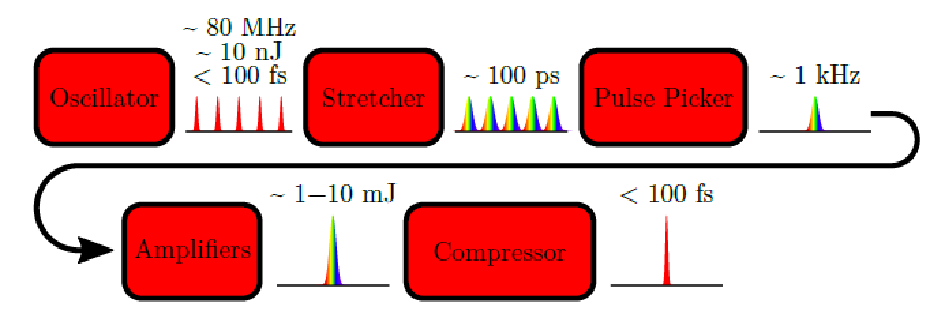
\includegraphics[width=1.0\textwidth]{figures/Beamline/CPA.pdf}
	\caption[Schematic of a CPA laser system]{Schematic of a CPA laser system. Adapted from \cite{kiesewetterDynamicsNearThresholdAttosecond2019}. }
	\label{fig:CPA}
\end{figure}

Many experiments can be done using these 800 nm pulses, however for the experiments described herein, wavelengths longer than 800 nm are required.  To  accomplish this, an optical parametric amplifier (OPA) is used to convert the 800 nm pulses into longer wavelengths, and this allows for wavelength tunability.  The basic idea of the OPA is to use nonlinear media to convert one larger photon (800 nm pump) into two smaller photons (1200-1600 nm signal and 1600-2400 nm idler) \cite{boydNonlinearOptics2008}.  The OPA used with the Spitfire is a commercial HE-TOPAS Prime from Light-Conversion.  The basic optical layout is shown in figure \ref{fig:OPA}, and consists of an initial white-light continuum generation followed by a series of nonlinear Beta Barium Borate (BBO) crystals.  These BBO crystals are optimized for difference frequency generation to amplify the 1200-1600 nm signal.  After these stages of amplification, the TOPAS can output a combine energy of 6 mJ for the combined signal and idler beams.  The pulse duration of these pulse can vary depending upon alignment and the wavelength selected, however it is generally around 60 fs. An example of a typical pulse in both intensity and spectrum is shown in figure \ref{fig:TOPAS_FROG}.  This was measured using a standard second-harmonic generation FROG setup which allows for full characterization of the pulse by extracting both the spectral amplitude and phase \cite{trebinoFrequencyresolvedOpticalGating2000}.

\begin{figure}
	\centering
	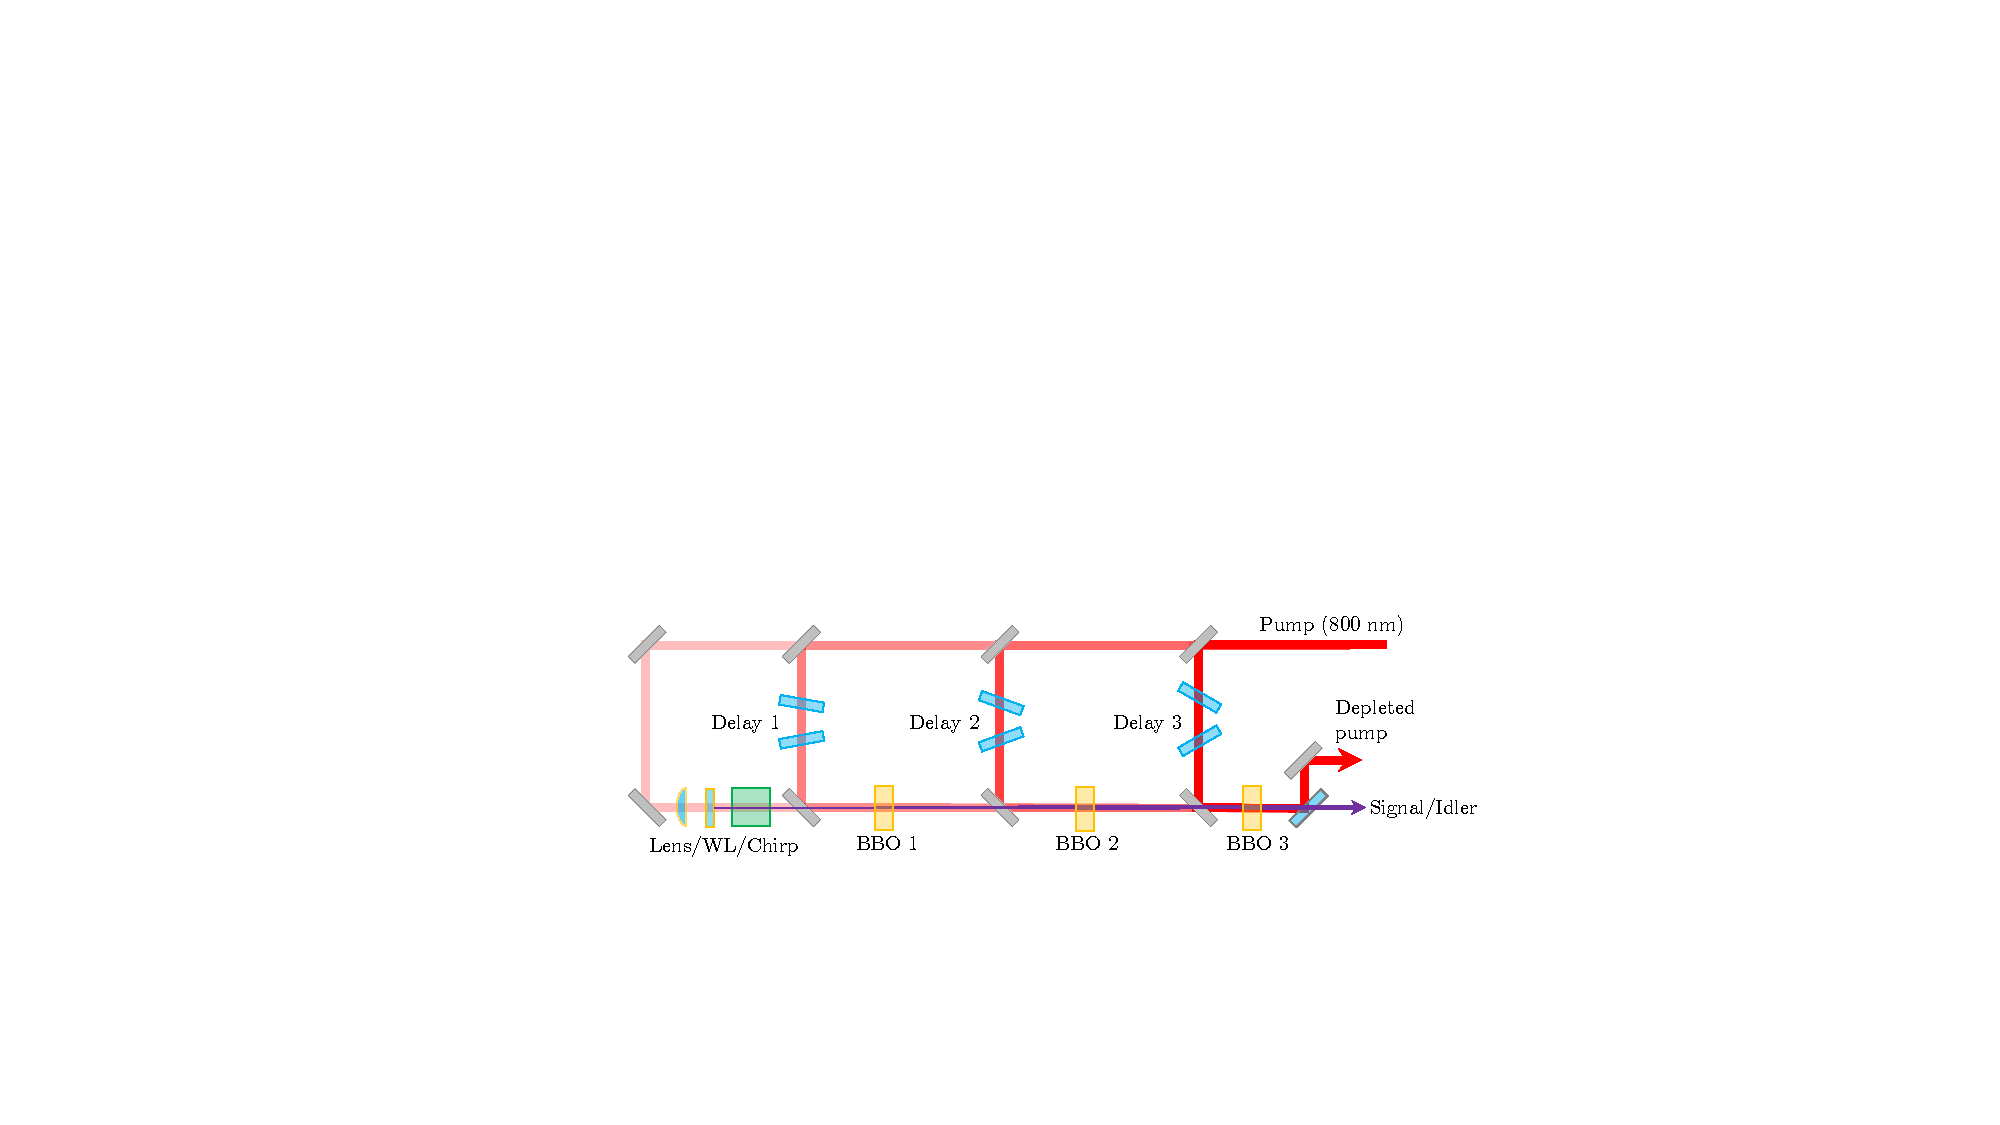
\includegraphics[width=1.0\textwidth]{figures/Beamline/OPA.pdf}
	\caption[Schematic of TOPAS]{Schematic of TOPAS OPA.  The pump beam enters with a pulse energy of 12 mJ before being split three times.  The lowest pulse energy beam is used to generate white light that is used to seed difference frequency generation in the successive BBO crystals.}
	\label{fig:OPA}
\end{figure}
\begin{figure}
	\centering
	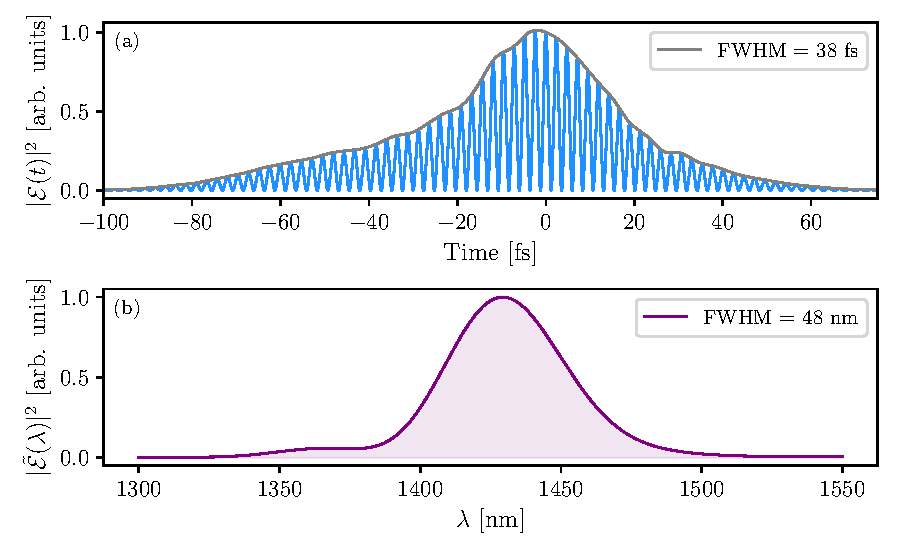
\includegraphics[width=1.0\textwidth]{figures/Beamline/TOPAS_FROG.pdf}
	\caption[Intensity and spectrum of TOPAS output for 1430 nm]{(a) Intensity profile of TOPAS output for a signal wavelength of 1430 nm. (b) Spectrum of TOPAS output for the same wavelength.}
	\label{fig:TOPAS_FROG}
\end{figure}

\section{Beamline Design}
\label{sec:full_beamline}
To begin discussion of the design of the TABLe, it is important to lay out the requirements that needed to be met when designing the apparatus. The primary feature common to all of the experiments that use TABLe is that they will involve XUV pulses that have bandwidth between 26 and 300 eV.  One of the challenges of working with wavelengths in this XUV region is that they require the use of high vacuum systems to perform most experiments.  The fundamental reason for this is due the fact that these wavelengths are ionizing radiation, and they will be quickly absorbed in air.  For example, at 50 eV the attenuation length\footnote{Attenuation length is given by the length that the intensity fall to $1/e$ as the beam propagates through a medium.} is approximately 50 $\mu$m for N$_2$ at 760 Torr \cite{henkeLowenergyXrayInteraction1982}.  Therefore, experiments must be performed in vacuum chambers generally in the high vacuum regime below $10^{-6}$ Torr.  An additional requirement is that these experiments are generally pump/probe experiments where the XUV pulse serves as either the pump or the probe and the other role is fulfilled by an IR pulse.  Thus, an interferometer needs to be designed where an input IR beam is split into two arms, one of which will have XUV generated in it.  A final requirement is that the beamline needs to be able to accommodate different end stations.  This is a critical feature because it greatly expands the capabilities of the apparatus beyond the initial experiments that the TABLe was commissioned for, namely transient absorption experiments.
\begin{figure}
	\centering
	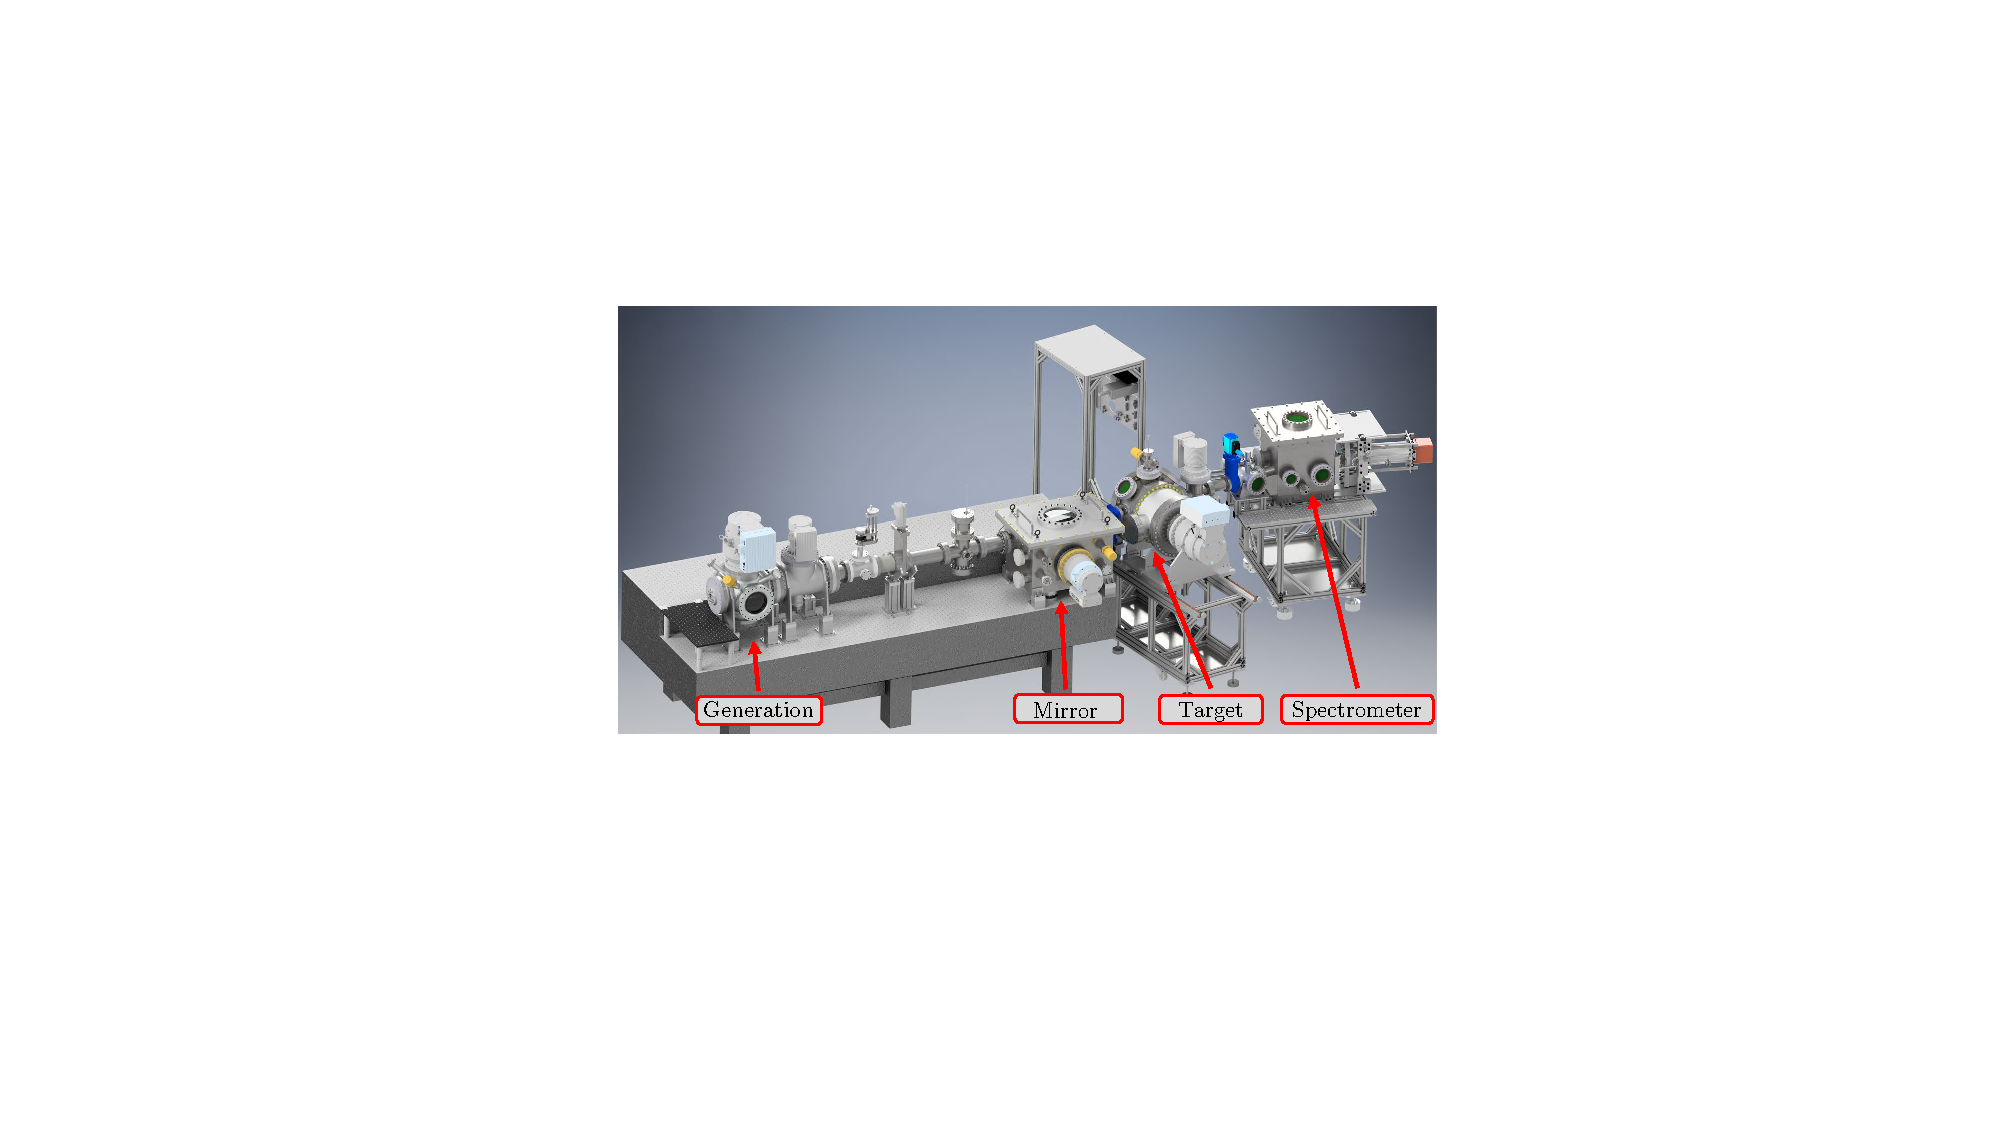
\includegraphics[width=1.0\textwidth]{figures/Beamline/CAD_beamline.pdf}
	\caption[Render of the TABLe]{Render of the Transient Absorption Beamline (TABLe).  The main vacuum chambers are highlighted.}
	\label{fig:CAD_render_TABLe}
\end{figure}
\begin{figure}
	\centering
	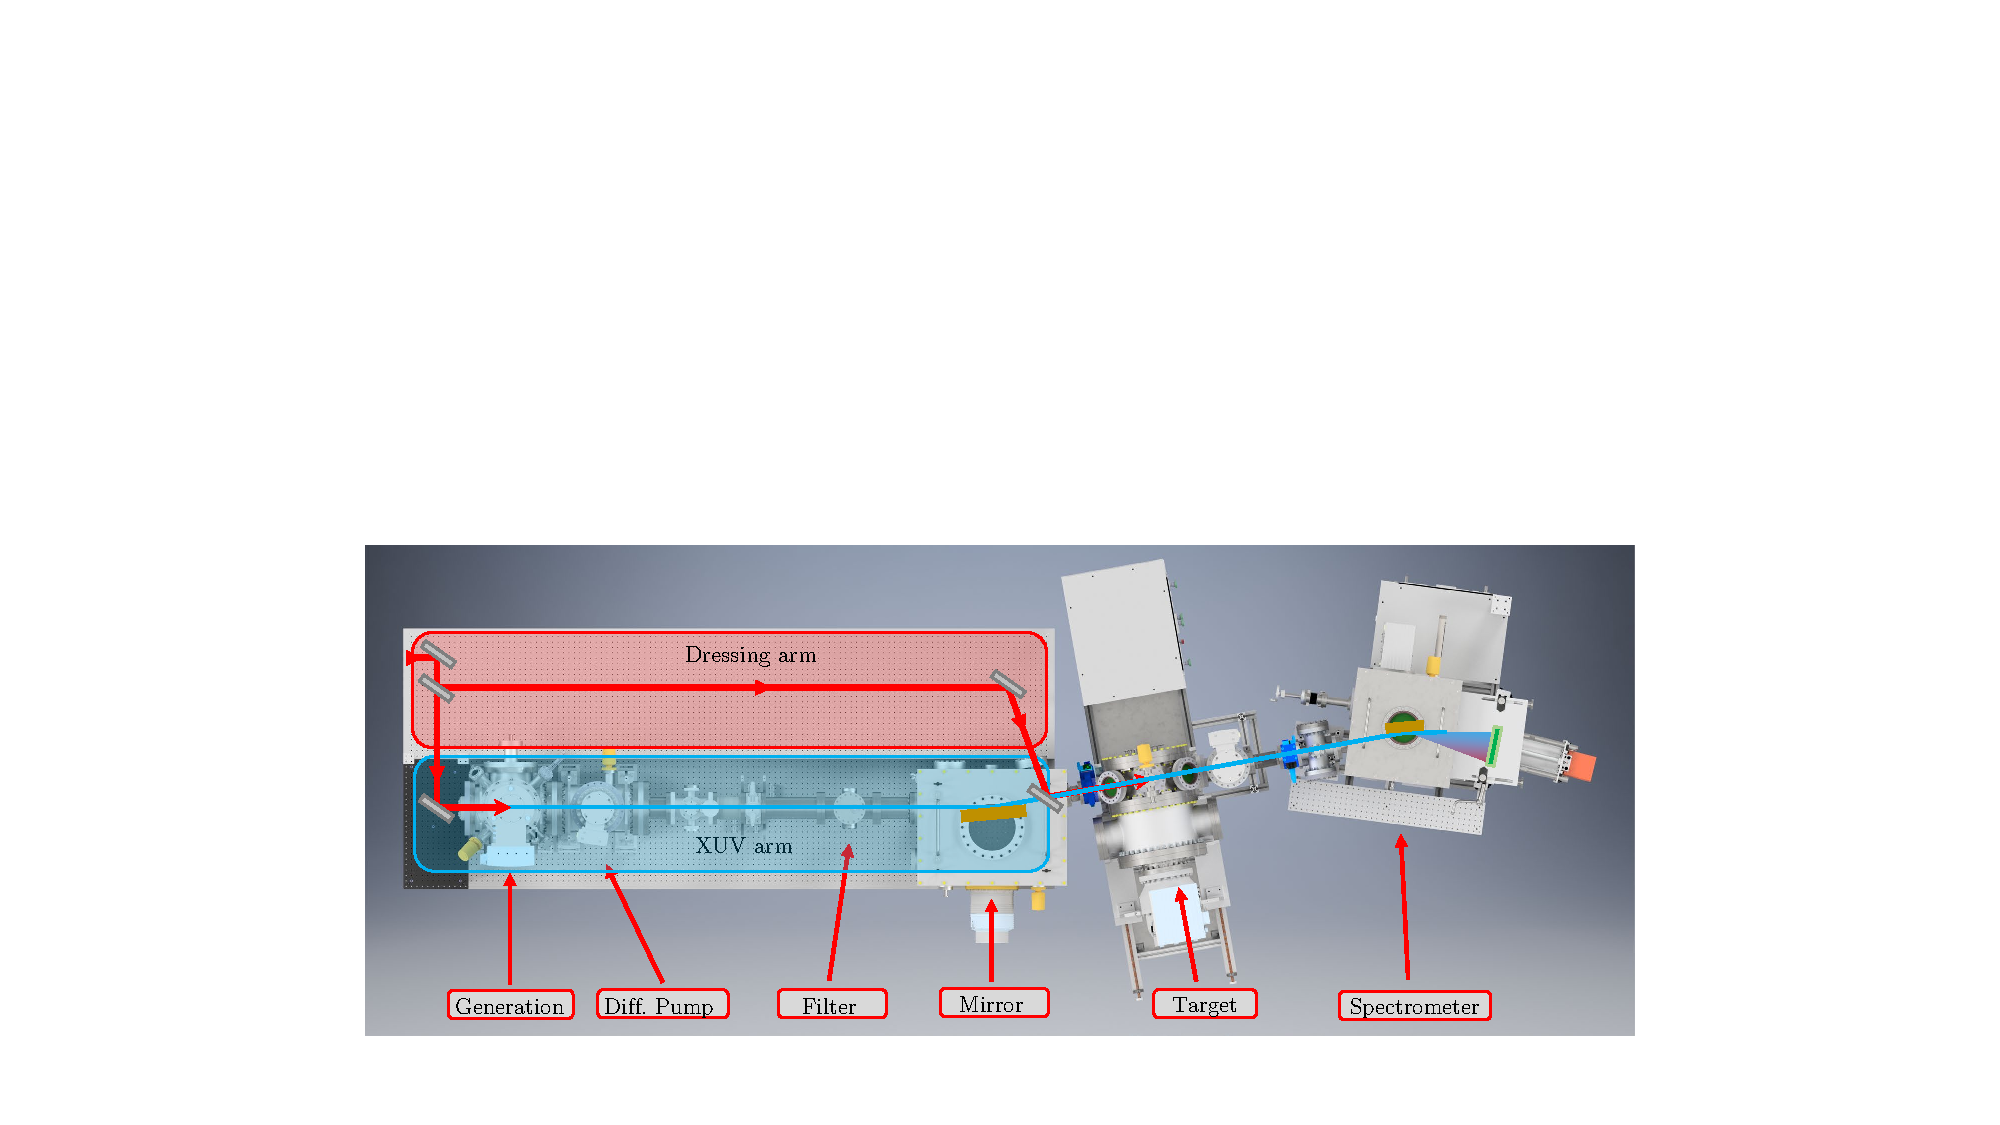
\includegraphics[width=1.0\textwidth]{figures/Beamline/CAD_beamline_top_view.pdf}
	\caption[Top-view render of the TABLe]{Top-view render of the Transient Absorption Beamline (TABLe).  The main vacuum chambers are highlighted, as well as the generation layout of the interferometer with the dressing and XUV arms.  Further details of the exact optical layout can be found in figure \ref{fig:beampath_sketch}.}
	\label{fig:CAD_beamline_top_view}
\end{figure}

The final design of the TABLe is shown in figure \ref{fig:CAD_render_TABLe}, and a top-view of the beamline with a rough schematic of the interferometer is shown in figure \ref{fig:CAD_beamline_top_view}. There are many details about the design and construction that will be left out of this dissertation, however they can be found in great abundance in Greg Smith's dissertation \cite{smithApplicationAttosecondTechniques2020}.  With that being said, the general structure of the vacuum system will be described first, and this consists of several main sections.  The first being the generation chamber which contains the gas source used for HHG.  This chamber is capable of accommodating a variety of gas sources consisting of continuous gas jets, pulsed gas jets, low pressure gas cells, and high pressure gas cells.  Each experiment has different requirements and focal geometries that make any one of these options more advantageous than the others, however the two options that will be used in this dissertation are the high pressure cell and the pulsed gas jet.  The details of the high pressure cell can be found in \cite{smithApplicationAttosecondTechniques2020}.  A picture of the high pressure cell with a laser filament going through it is shown in figure \ref{fig:HPGC_filament}.  The distinguishing feature of the high pressure cell is its ability to achieve interaction pressures up to several bar through the use of a pair concentric tubes that the allow for differential pumping.  The primary disadvantages are the difficulty in initial alignment and the restrictive set of four holes that the laser must propagate through.  This make the high pressure cell untenable for some experiments, such as those described in Chapters \ref{chap:two_source}, \ref{chap:refractive_index}, and \ref{chap:CATS}.  An alternative to the gas cell is the pulsed gas jet.  This work by using a piezoelectric actuator to block gas from exiting a gas nozzle and only let out a pulse of gas at a fixed frequency and duty cycle.  This operation mode means that the average background pressure within the vacuum is lower than just a simple continuous gas jet operation, but the interaction pressure can be the same.  A picture of the pulsed jet in operation is shown in figure \ref{fig:piezo_jet}.
\label{sec:gas_source}
\begin{figure}
	\centering
	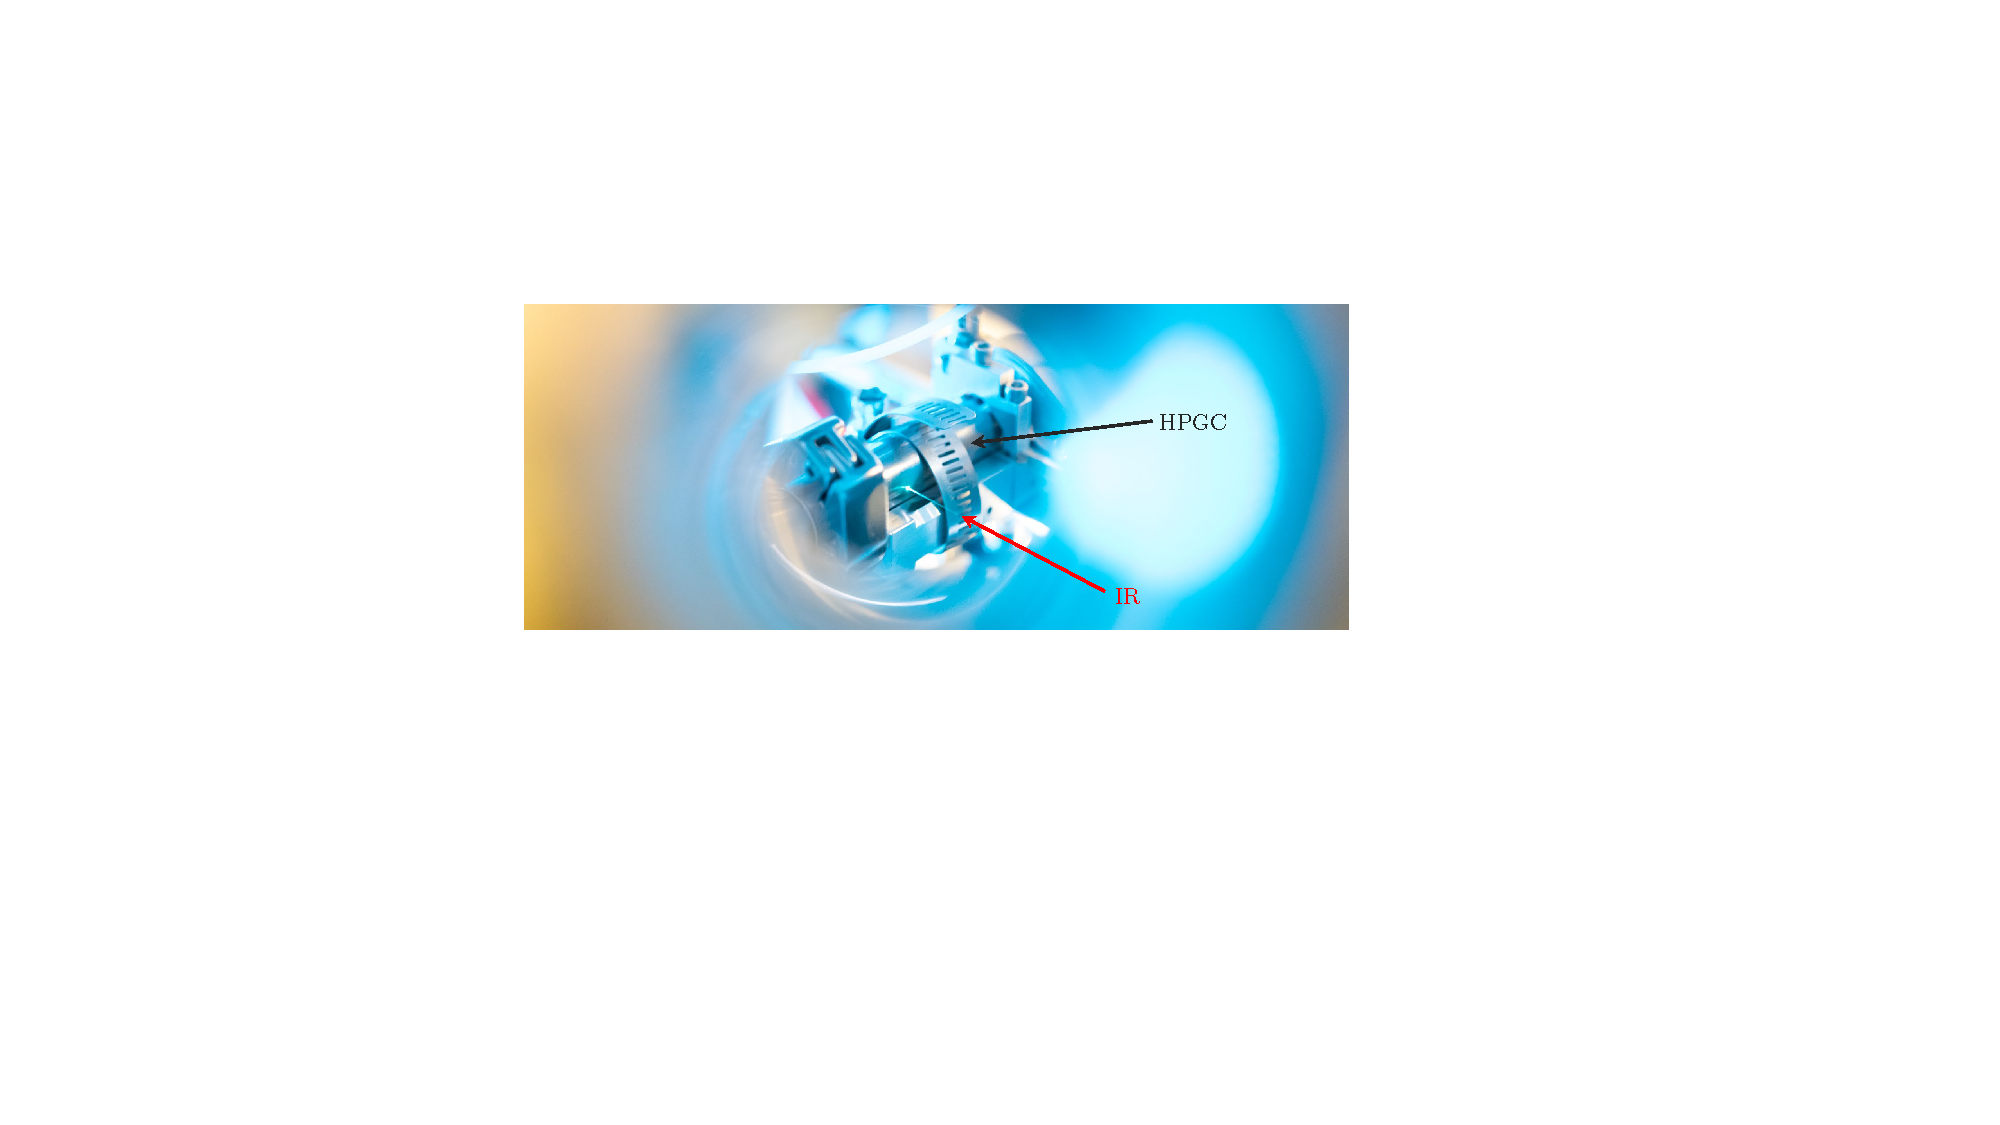
\includegraphics[width=0.8\textwidth]{figures/Beamline/HPGC.pdf}
	\caption[Image of laser passing through HPGC]{Camera image of IR laser filament pass through the high-pressure gas cell (HPGC) during alignment at atmospheric conditions.}
	\label{fig:HPGC_filament}
\end{figure}


Following a differential pumping section, there is a metallic spectral filter assembly.  This is used to place a metallic filter that is generally on the order of a few hundred nanometers into the beam path of the XUV.  The primary reason for this is to block the co-propagating IR field that is used to generate the XUV pulse.  However, it can also be used to shape the spectrum and phase of the XUV pulse to suit the experimental requirements \cite{chiniGenerationCharacterizationApplications2014}.  The transmission function of three of the most common filter materials is shown in figure \ref{fig:filters}.  As can be clearly seen, different materials have significantly different bandpass windows, and this is due to each elements atomic structure and the transition energy of the core level.  For example, Al is the filter that is most commonly used for these experiments, and it transmits reasonably well below the $L$-edge which occurs at 72.3 eV, however it strongly absorbs above this energy.
\begin{figure}
	\centering
	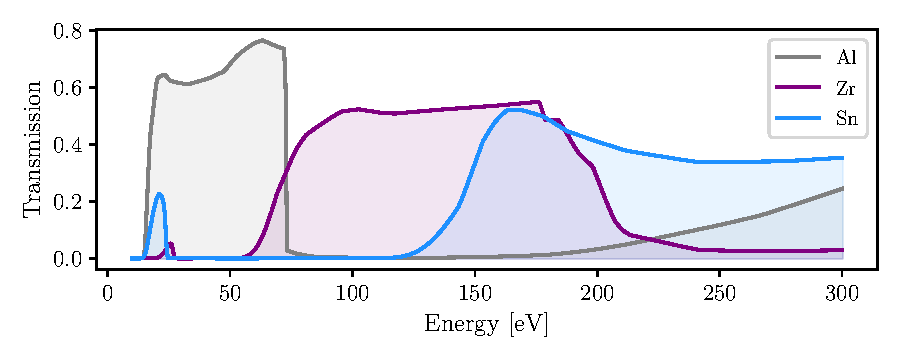
\includegraphics[width=0.9\textwidth]{figures/Beamline/filters.pdf}
	\caption[Transmission of several metallic filters]{Transmission as a function of photon energy for several metallic filters.  All filters are 200 nm thick.}
	\label{fig:filters}
\end{figure}

The next main section of the TABLe that must be described is the mirror chamber.  This section houses the primary XUV focusing optic, the ellipsoidal mirror.  Again, much greater detail can be found in \cite{smithApplicationAttosecondTechniques2020}, however the key features of this special optic will be discussed here.  A significant challenge with working in this energy range is the lack of efficient and broadband optics.  This is due to the strong absorption by most materials when they are used near normal incidence.  There are two main methods that have been employed to overcome this: grazing incidence optics or multilayer optics \cite{attwoodSoftXraysExtreme2000}.  Each have their advantages and disadvantages, but generally grazing incidence optics operate over a much larger bandwidth.  This was a key design criteria for the TABLe, so a grazing incidence optic was selected to refocus the XUV beam.  There are several designs that can be used to refocus a beam using a grazing incidence optics, and the one that was selected was the ellipsoidal mirror.  The significant advantage of this type of optic is that is can re-image a point source aberration free with demagnification.  The geometric optics principle behind this is highlighted in figure \ref{fig:ellipsoid}.  The ellipsoid that was chosen for the TABLe has an entrance arm of 2250 mm and an exit arm of 750 mm, thus giving a demagnification of 3.  This allows for smaller XUV spot sizes to be used.
\begin{figure}
	\centering
	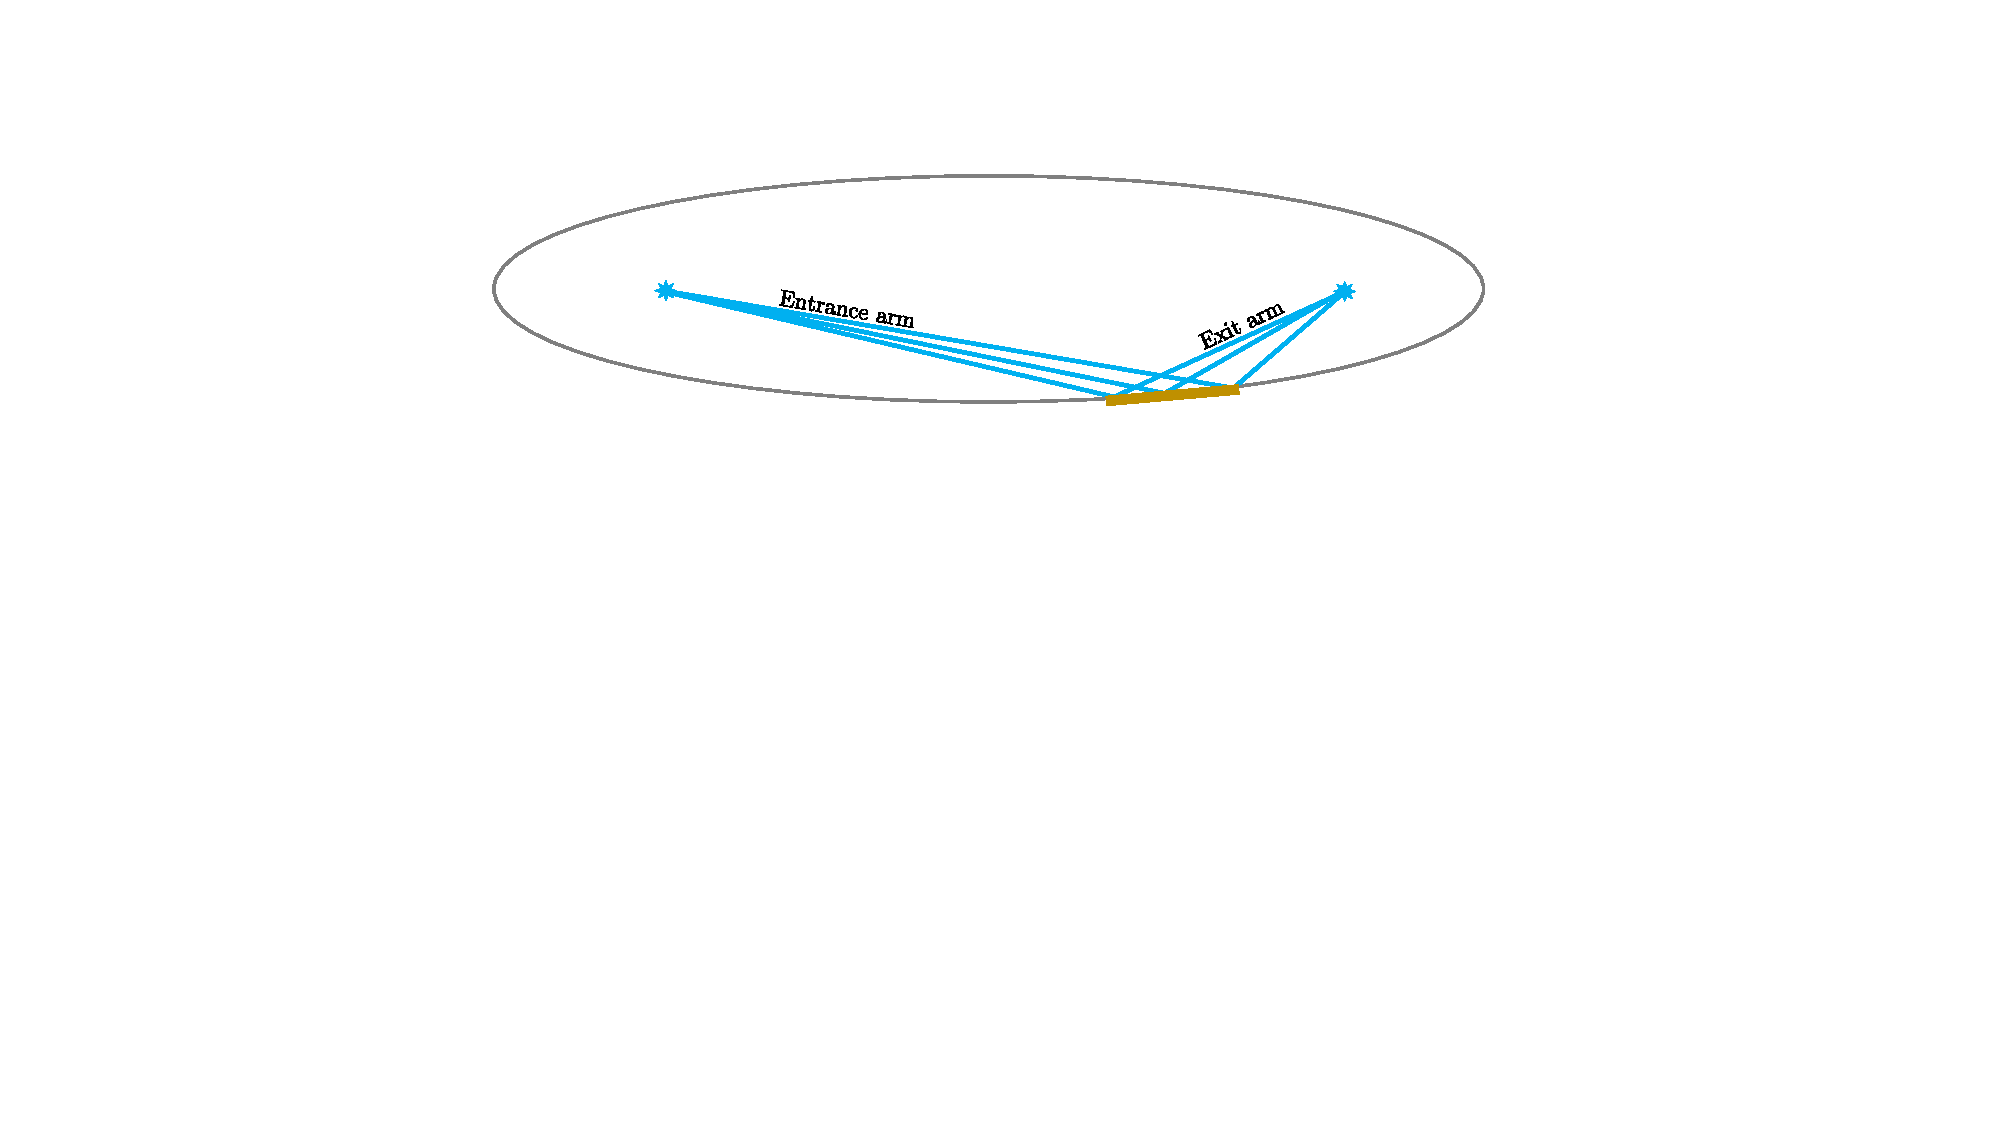
\includegraphics[width=0.8\textwidth]{figures/Beamline/ellipsoid.pdf}
	\caption[Schematic of ellipsoidal mirror]{Schematic of ellipsoidal mirror.  From geometric optics, the ellipsoidal mirror will focus all rays from a point source at one foci of the ellipse to the other foci.  The ratio of the exit arm to the entrance arm is the magnification provided by the mirror.}
	\label{fig:ellipsoid}
\end{figure}

The next major section of the TABLe is the target chamber.  As the name implies, this is where the sample of interest for an experiment is placed.  This chamber is capable of housing both condensed matter samples in the form of free standing membranes and a gas cell to perform gas phase measurements.  The two configurations that the target chamber can operate in is shown in figure \ref{fig:gas_solid_sample_holder}. 
\begin{figure}
	\centering
	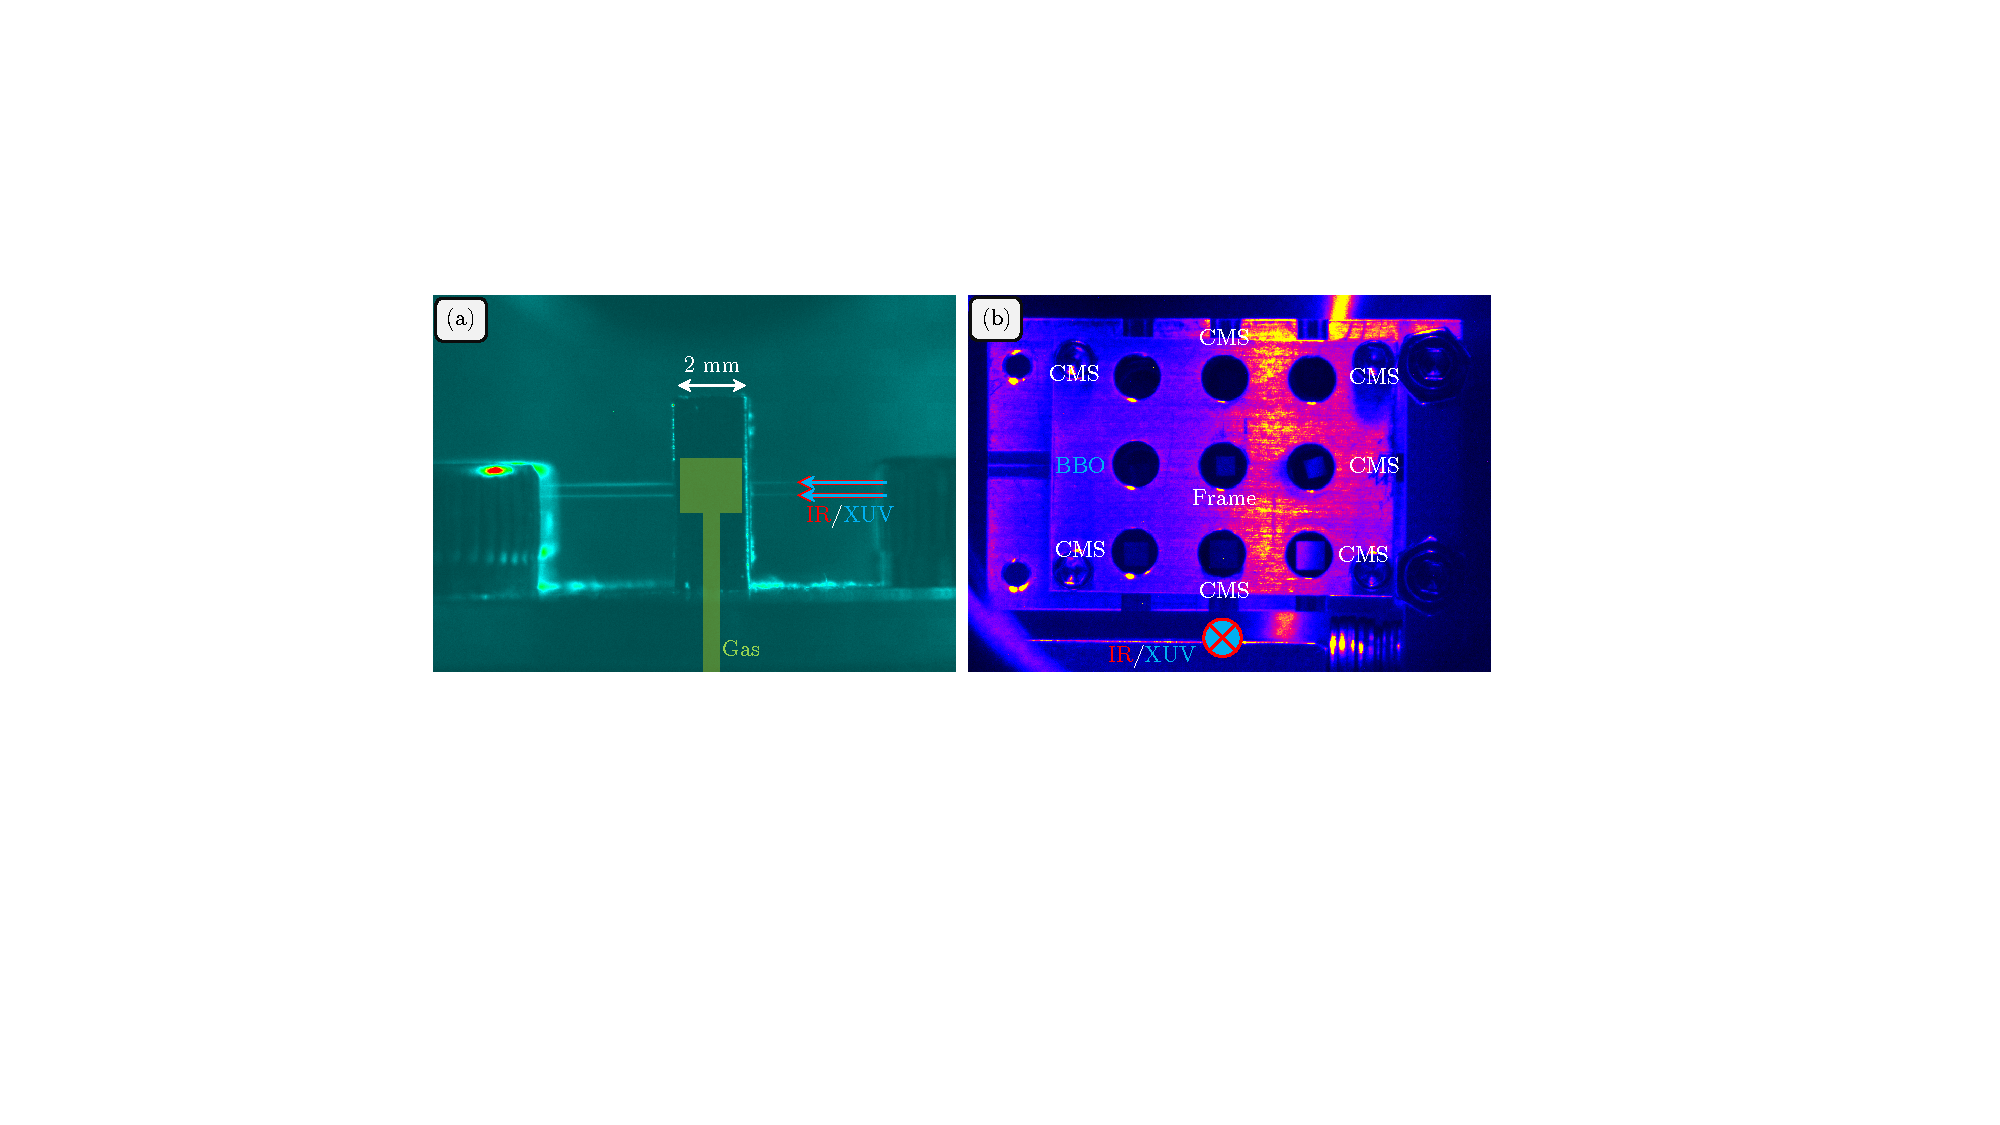
\includegraphics[width=0.9\textwidth]{figures/Beamline/gas_solid_sample_holder.pdf}
	\caption[Camera image of target gas cell and condensed matter sample holder]{(a) Camera image of the gas cell used for gas phase experiments. Two sources IR sources are generating a filament. Image was taken while chamber was vented and at ambient pressure. (b) Camera image of the condensed matter sample holder.  This was taken \textit{in-situ} while under vacuum.  The sample holder is generally configured to carry six condensed matter samples (CMS), one BBO to find temporal overlap, and one empty frame to perform knife-edge measurements.  The IR/XUV beams propagate into the page for this image.}
	\label{fig:gas_solid_sample_holder}
\end{figure}

Finally, the last major component of the TABLe that needs to be discussed is the photon spectrometer.  This home-built spectrometer was commissioned to perform the experiments described in this dissertation as well as those described in \cite{smithApplicationAttosecondTechniques2020}.  The design criteria that this spectrometer had to meet was that it had to be a high resolution spectrometer covering a spectral range from 20 eV all the way through the Carbon $K$-edge at 284 eV.  This was chosen because of eventual plans to perform transient absorption experiments in the water-window at the Carbon $K$-edge, while still maintaining the ability to do more reasonable experiments at lower photon energies in the 20 - 100 eV range.

This is a massive bandwidth to cover with high resolution, so the decision was made to use two different grating to cover this full spectral range.  The gratings that were selected are concave spherical variable line spaced (VLS) gratings produced by Hitachi.  A schematic of the grating is shown in figure \ref{fig:Hitachi_gratings}, and the relevant design parameters for the gratings are given in table \ref{tab:vls_gratings}.  The advantage of a VLS grating design is that they combine the focusing and dispersive optics that are generally needed into a single optic that performs both functions.  Furthermore, these gratings are designed to focus a specific spectral bandwidth onto a plane (as opposed to the typical Rowland circle \cite{rowlandConcaveGratingsOptical1883, pedrottiIntroductionOptics2007}), and this means that a large bandwidth can be in focus on a detector at a single position.  This can be seen in figure \ref{fig:VLS_flat_field} where the focal plane for a range of wavelengths is shown for both grating. This is calculated using the relationship between the entrance $r$ and exit arm $r'$ at an incidence angle $\theta_i$ is given by
\begin{equation}
	r' = \frac{r R (\cos\theta_r)^2}{m\lambda\sigma_0 b_2 + r(\cos\theta_i + \cos\theta_r) - R(\cos\theta_i)^2}
\end{equation}
where $R$ is the radius of curvature, $m$ is the diffraction order, $\theta_r$ is given by
\begin{equation}
	\sin\theta_i + \sin\theta_r = m\sigma\lambda,
\end{equation}
and $b_2$, $\sigma$, $\sigma_0$ are given by 
\begin{equation}
	\sigma(w) = \frac{\sigma_0}{1 + \frac{2b_2}{R}w + \frac{3b_3}{R^2}w^2 + \frac{4b_4}{R^3}w^3 + ...}
\end{equation}
which is the groove density along the face of the grating $w$ \cite{polettoGrazingincidenceFlatfieldSpectrometer2001, haradaMechanicallyRuledAberrationcorrected1980, haradaOptimumDesignGrazingincidence1999}.
\begin{figure}
	\centering
	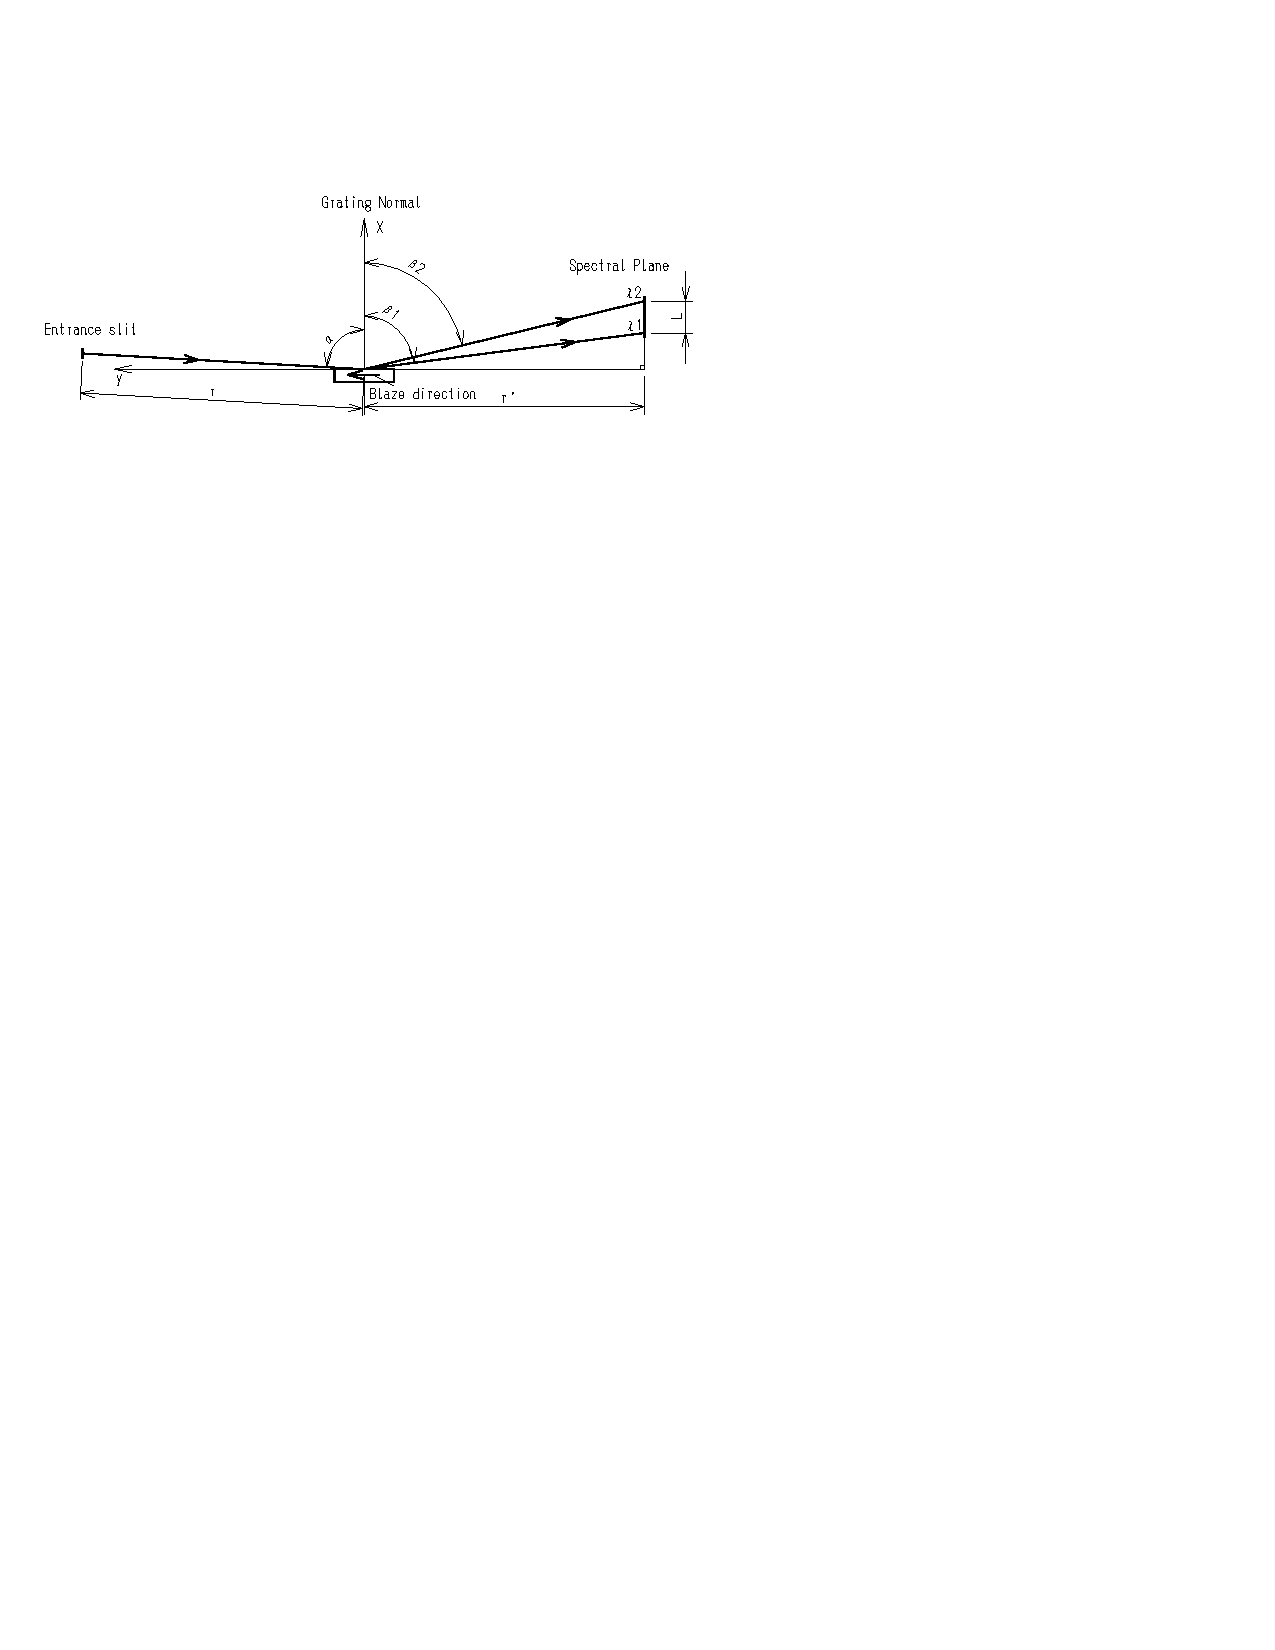
\includegraphics[width=0.8\textwidth]{figures/Beamline/Hitachi.pdf}
	\caption[Schematic of VLS grating]{Schematic of VLS grating with the design parameters $r$ (distance from slit to center of grating), $r'$ (distance from center of grating to image plane), and $L$ (the length of the spectral range that is in focus between $\lambda_1$ and $\lambda_2$).}
	\label{fig:Hitachi_gratings}
\end{figure}
\begin{table}[]
	\centering
	\begin{tabular}{|c|c|c|c|c|c|c|c|}
		\hline\hline
		lines/mm & \begin{tabular}[c]{@{}c@{}}Blaze \\ $\lambda$ {[}nm{]}\end{tabular} & $\alpha$ & r {[}mm{]} & r' {[}mm{]} & $\beta_1$ & $\beta_2$ & $\lambda_1$-$\lambda_2$ \\ \hline
		1200     & 10                                                                  & 87       & 237        & 235.3       & -83.04    & -77.07    & 5-20                    \\ \hline
		2400     & 1.5                                                                 & 88.7     & 237        & 235.3       & -85.81    & -81.01    & 1-5                     \\ \hline\hline
	\end{tabular}
	\caption[Parameters of Hitachi VLS gratings]{Parameters of Hitachi VLS gratings.}
	\label{tab:vls_gratings}
\end{table}

\begin{figure}
	\centering
	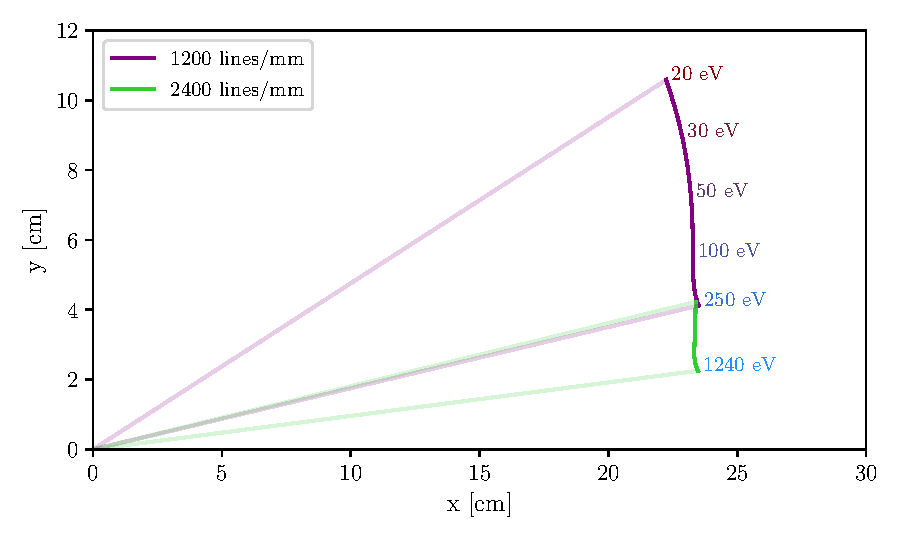
\includegraphics[width=0.9\textwidth]{figures/Beamline/VLS_flat_field.pdf}
	\caption[Flat field of VLS gratings]{Flat fields of the two VLS grating that comprise the photon spectrometer.  The $x$ axis is parallel to the face of the grating, and the $y$ axis is perpendicular to the grating face.  The center of the grating is located at (0,0).  Incidence angle and entrance arm are those provided in table \ref{tab:vls_gratings}.}
	\label{fig:VLS_flat_field}
\end{figure}




Another design criteria for this spectrometer was that it had to be able to be used on a variety of different systems.  The modular design of the TABLe meant that this spectrometer could be removed from the TABLe and brought to a different light source.  This entails that the entrance arm could be different from the one specified by the manufacturer depending upon the system that is installed in.  To account for this change in entrance arm, the angle of the grating can be changed from the specified one to recover the flat field condition.  This can be seen for both gratings in figure \ref{fig:variable_flat_field}.  Of course, one issue with this approach is that even though the flat field can be recovered, the grating efficiency changes as a function of angle.  This can be done numerically, and there are many packages available to perform these calculations. The grating efficiency for the 1200 lines/mm grating was calculated in \cite{hageDevelopmentXUVSpectrometer}, and the results are shown in figure \ref{fig:grating_efficiency}.  As can be clearly seen, the efficiency changes non-trivially as a function of grazing angle for a given wavelength.  Thus, depending upon the position of the detector and the photon energy of interest, there is a different incident angle that can be selected to optimize the grating efficiency.
\begin{figure}
	\centering
	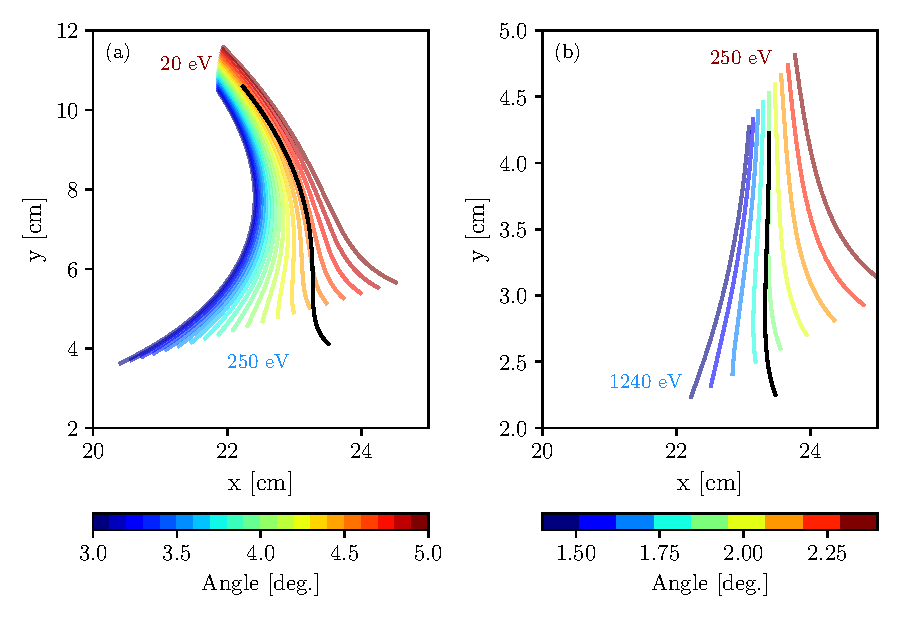
\includegraphics[width=0.9\textwidth]{figures/Beamline/variable_flat_field.pdf}
	\caption[Flat field of both VLS gratings as a function of input angle]{Flat field calculated as a function of incident angle for an entrance arm of 1.5 m.  The flat field for the manufacturers specified entrance arm of 0.237 m is shown in black. (a) is for the 1200 lines/mm VLS grating and (b) is for the 2400 lines/mm VLS grating. The $x$ axis is parallel to the incident light, and teh $y$ axis is perpendicular to the incident light.}
	\label{fig:variable_flat_field}
\end{figure}

\begin{figure}
	\centering
	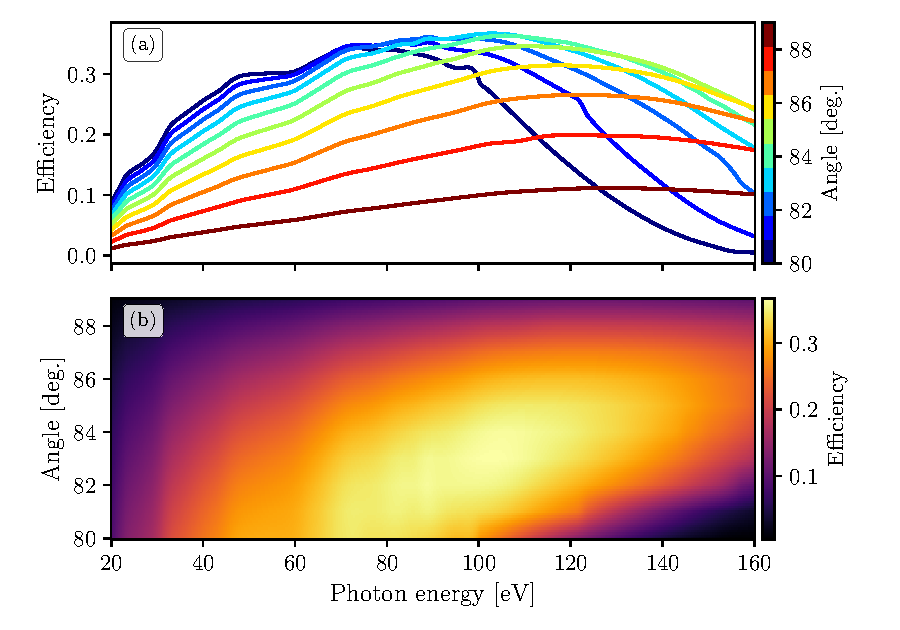
\includegraphics[width=0.9\textwidth]{figures/Beamline/grating_efficiency.pdf}
	\caption[VLS grating efficiency as a function of incident angle and photon energy]{Calculated VLS grating efficiency as a function of grazing angle and photon energy.  Shown as a series of line outs in (a) and as an interpolated heat map in (b).  Data is obtained from \cite{hageDevelopmentXUVSpectrometer}.}
	\label{fig:grating_efficiency}
\end{figure}

\begin{figure}
	\centering
	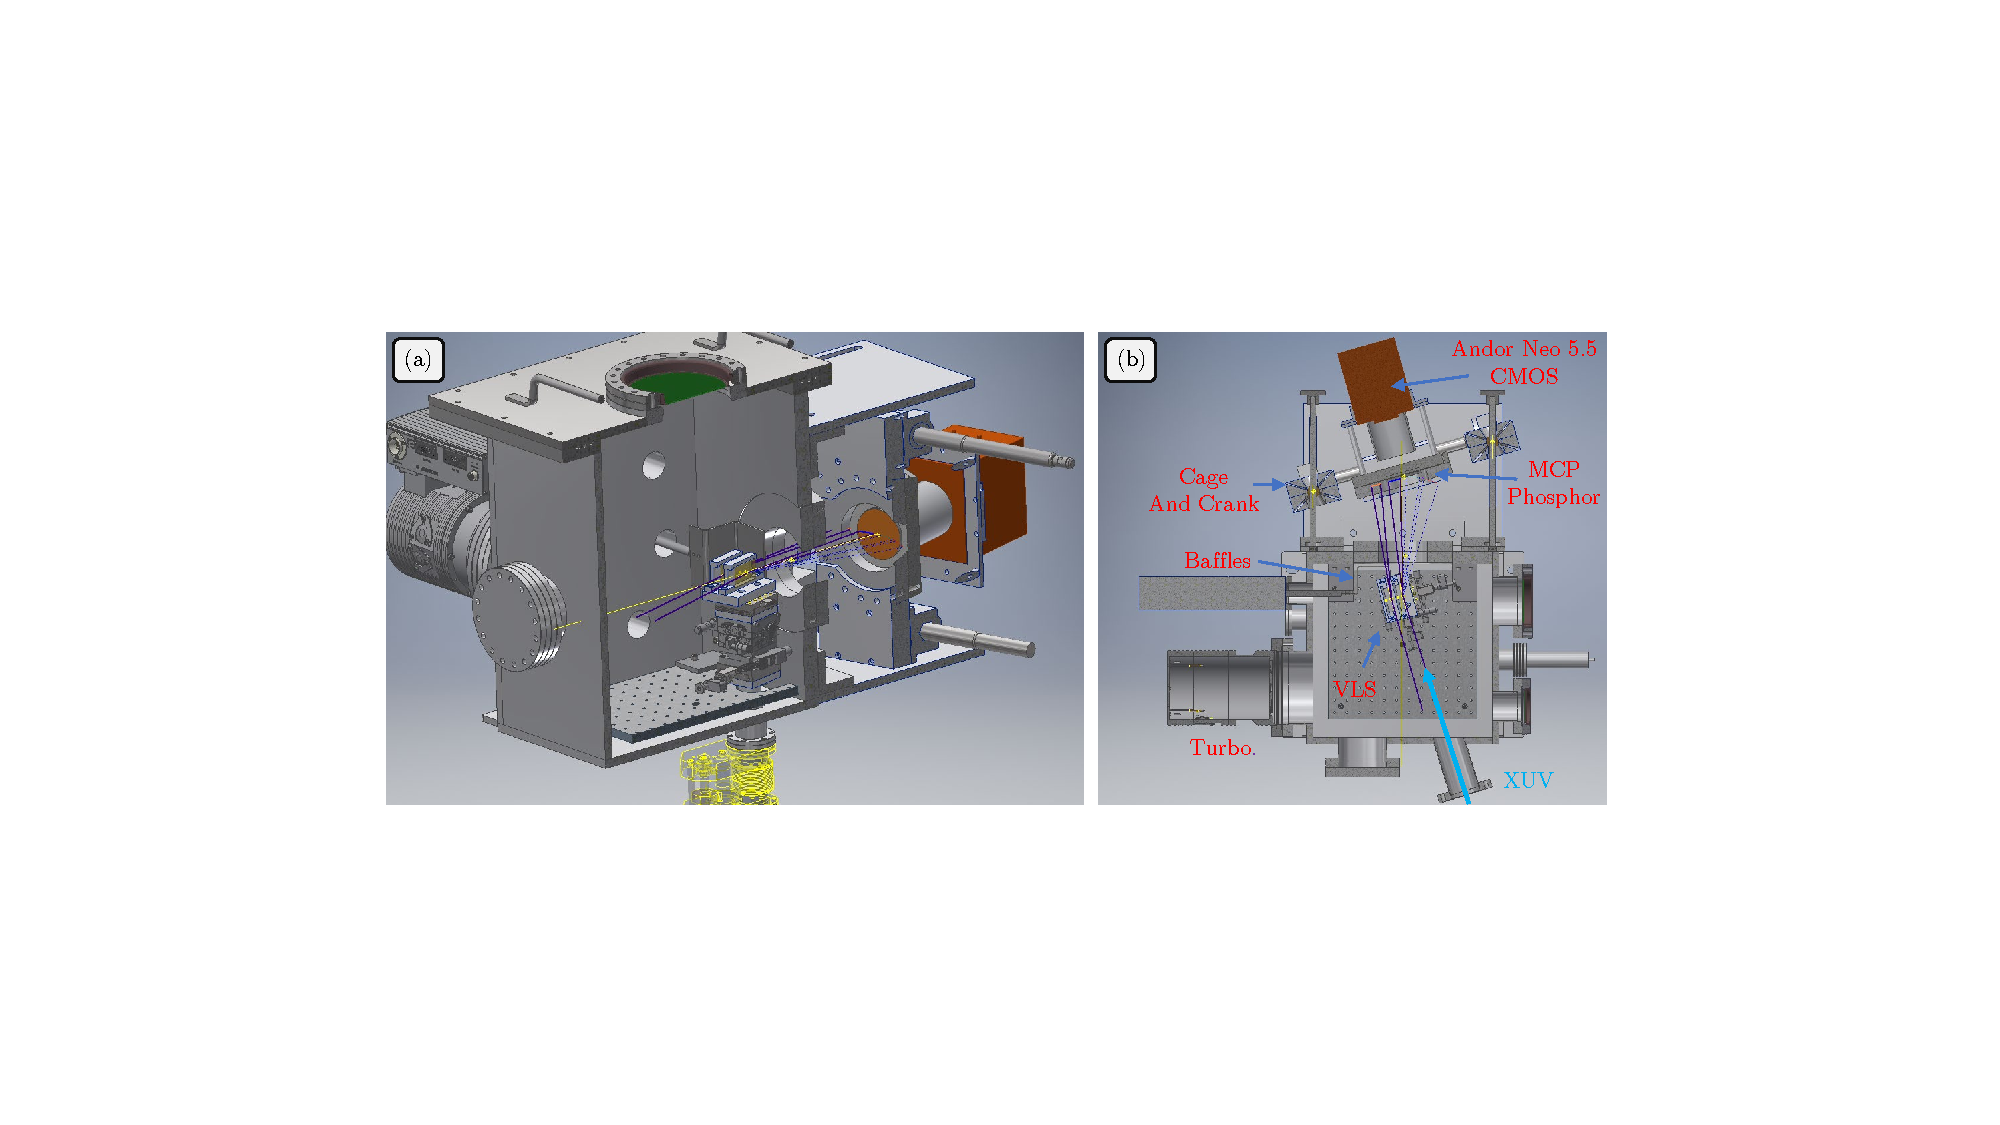
\includegraphics[width=0.9\textwidth]{figures/Beamline/CAD_spectrometer.pdf}
	\caption[CAD render of the TABLe spectrometer]{Render of the spectrometer showing a side-view (a) and a top-view (b).}
	\label{fig:CAD_spectrometer}
\end{figure}

Now it is time to move on to the actual design of the spectrometer, and a render of the spectrometer is shown in figure \ref{fig:CAD_spectrometer}. This design has the capability to switch between the two diffraction gratings while under vacuum through the use of 6-axis motorized control.  The detector consists of a 75 mm imaging quality micro-channel plate (MCP) and phosphor that is mounted on an 8" ConFlat flange.  The output of the phosphor is re-imaged onto an Andor Neo 5.5 CMOS camera using a 50 mm focal length lens.  The MCP was selected over a direct detection XUV CCD camera because of the much larger detector area that can be achieved using an MCP. To position this detector along the focal plane for each grating, a custom manipulator was developed, and this manipulator is referred to as the cage and crank.  It consists of three screws that allow for the tilt and translation of the detector while the chamber is under vacuum.  This allows for optimization of the resolution in different parts of the harmonic spectrum based upon the experimental needs.  An example of the phosphor output is shown in figure \ref{fig:spectrometer_output} (a) for a case where the phosphor emission was bright enough that it could be easily seen by eye, and an example of a typical image taken by the Andor camera is shown in figure \ref{fig:spectrometer_output} (b).  These images constitute the basis of all of the experiments that are described within this dissertation, and there are a couple of key features that are important to highlight.  As a consequence of selecting VLS gratings, the resulting spectrum that is measured is only focused along the spectral dimension, as shown in figure \ref{fig:spectrometer_output} (b), and the other dimension, generally referred to as the spatial dimension,  is unfocused and allows for the measurement of the spatial profile of the XUV beam as a function of energy.  This allows for unique measurements to be performed that involve the spatial interference of two XUV beams, and this capability is what enables the experiments in Chapters \ref{chap:two_source}, \ref{chap:refractive_index}, and  \ref{chap:CATS}.


\begin{figure}
	\centering
	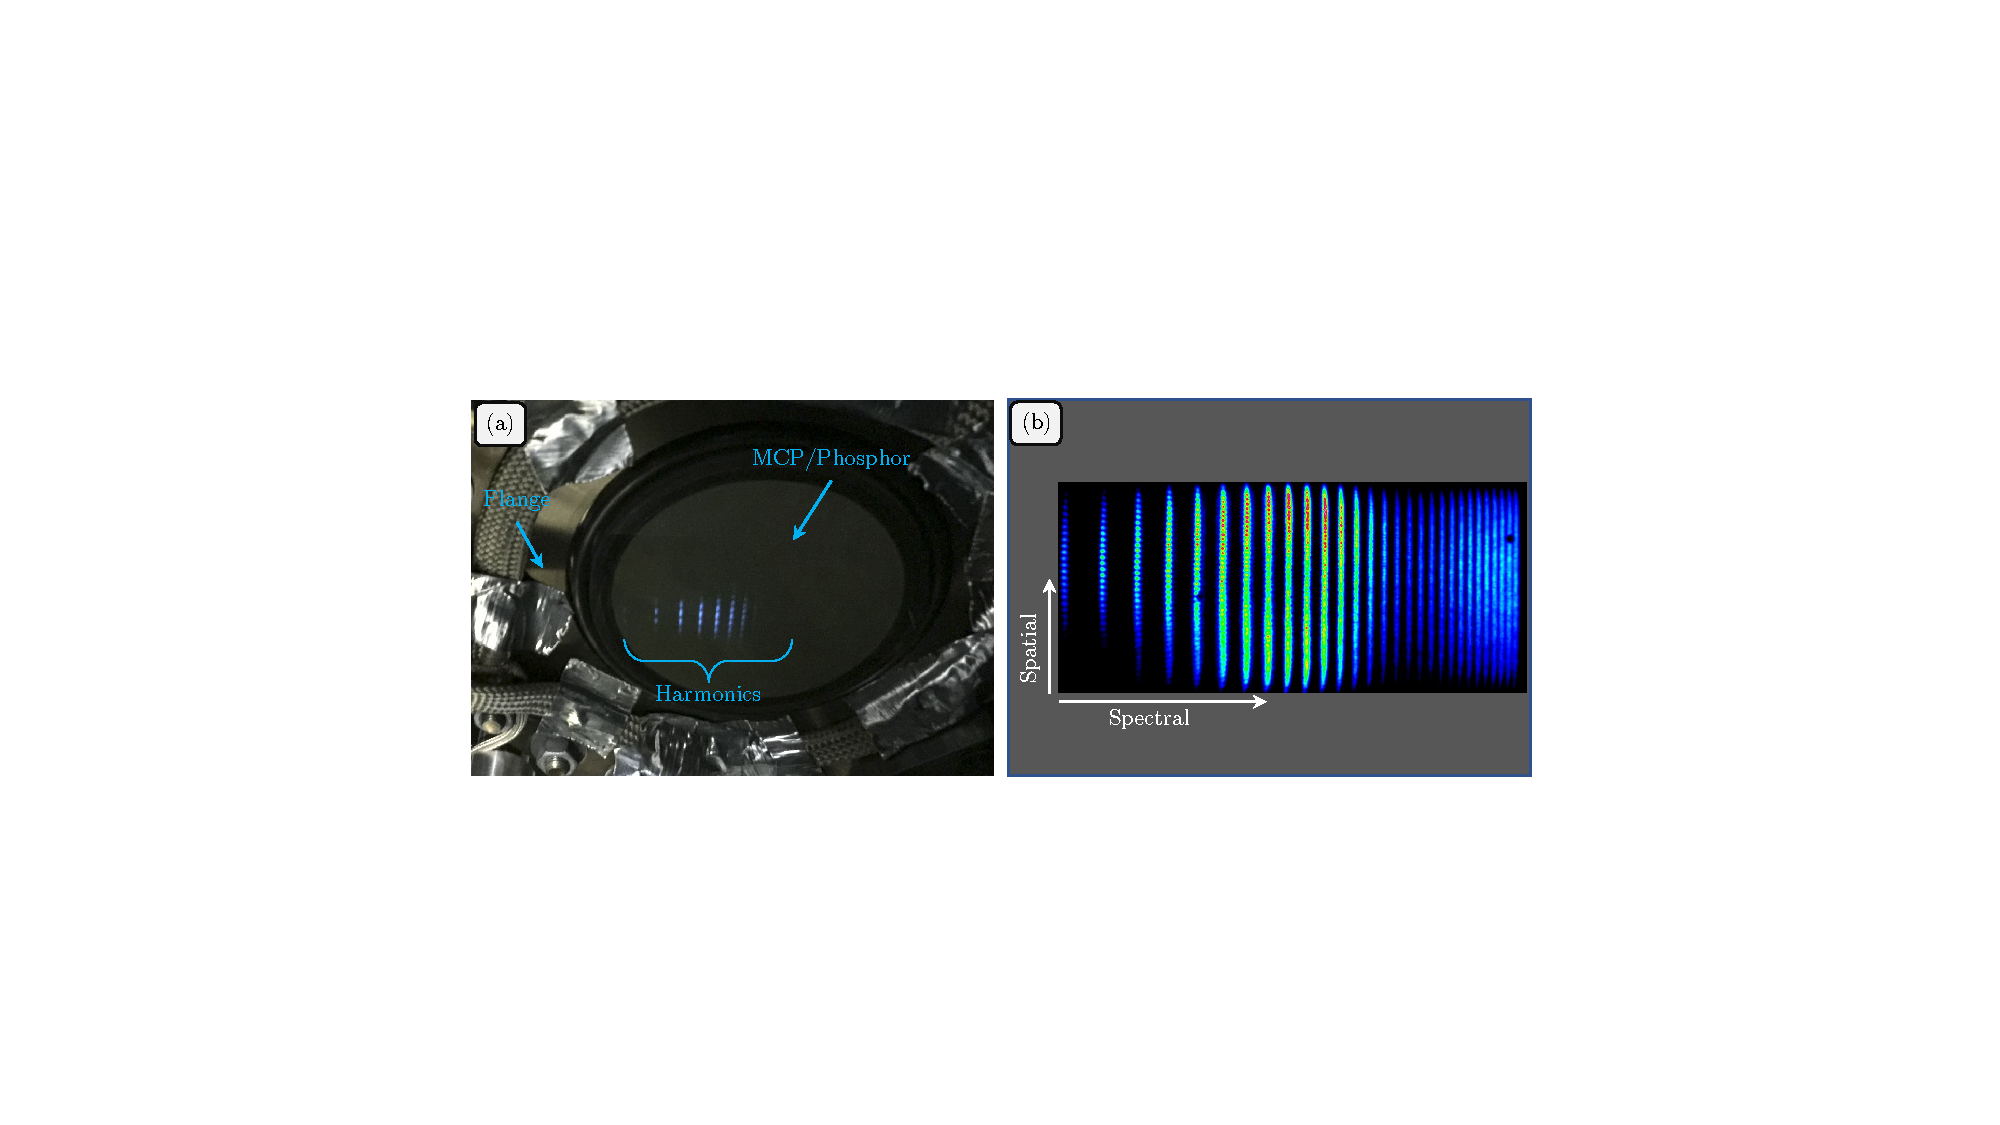
\includegraphics[width=0.9\textwidth]{figures/Beamline/spectrometer_output.pdf}
	\caption[Image of phosphor output of high harmonics generated from two sources and sample data image]{(a) Camera image of the output of the phosphor screen.  Harmonics are visible by eye.  (b) Sample data image collected from the Andor high-resolution camera.  Spatial and spectral structure of the XUV APT can be seen.}
	\label{fig:spectrometer_output}
\end{figure}

Finally, the last important consideration of the spectrometer is its maximum achievable resolution.  This can be done by calculating the energy difference between two points that are separated by the effective pixel size along the flat field curve.  This calculation is shown in figure \ref{fig:grating_resolution} for both gratings.  In the energy range of 20-80 eV, the resolution $\Delta E/E$ of the 1200 lines/mm grating ranges from $1\times10^{-3}$ to $2\times10^{-3}$.  This resolution is fundamentally limited by the effective pixel size, and it can be improved by a factor of 4 if a different re-imaging lens is used for the Andor camera. Further resolution improvements can be made by using a direct detection XUV CCD camera with smaller pixel sizes.
\begin{figure}
	\centering
	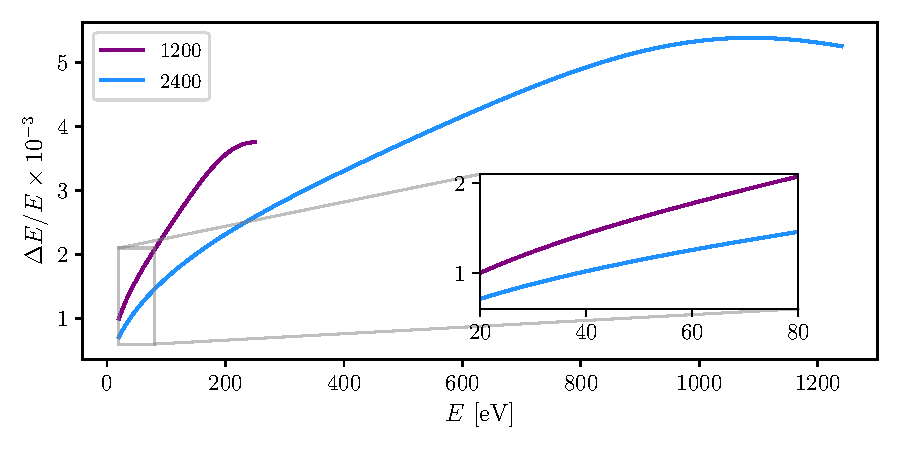
\includegraphics[width=0.9\textwidth]{figures/Beamline/grating_resolution.pdf}
	\caption[Maximum achievable resolution for VLS gratings]{Maximum achievable resolution for the 1200 and 2400 lines/mm VLS gratings. Calculated using an effective pixel size of 48 $\mu$m.  Inset shows the spectral region that will be important for the experiments described herein.}
	\label{fig:grating_resolution}
\end{figure}



\section{Optical layout}
\label{sec:optical_layout}

Now that the design of the TABLe has been covered, attention can now be turned to the optical layout of the TABLe.  As stated previously, the TABLe is designed around performing pump/probe experiments using both XUV and IR pulses.  This is done by building a Mach-Zehnder interferometer where one arm is IR and the other arm is used to generate the XUV APT.  The optical layout that was implemented is shown in figure \ref{fig:beampath_sketch}.  This setup was designed to use the signal wavelengths from the TOPAS over the 1250-1550 nm range, and it can accommodate a wavelength change within this range with minimal adjustment of the interferometer.  In the following sections several major components that determine the interferometer performance will be highlighted, and the two different XUV generation schemes that are used will be described in Chapter \ref{chap:two_source} and \ref{chap:ATS}.

\begin{sidewaysfigure}
	\centering
	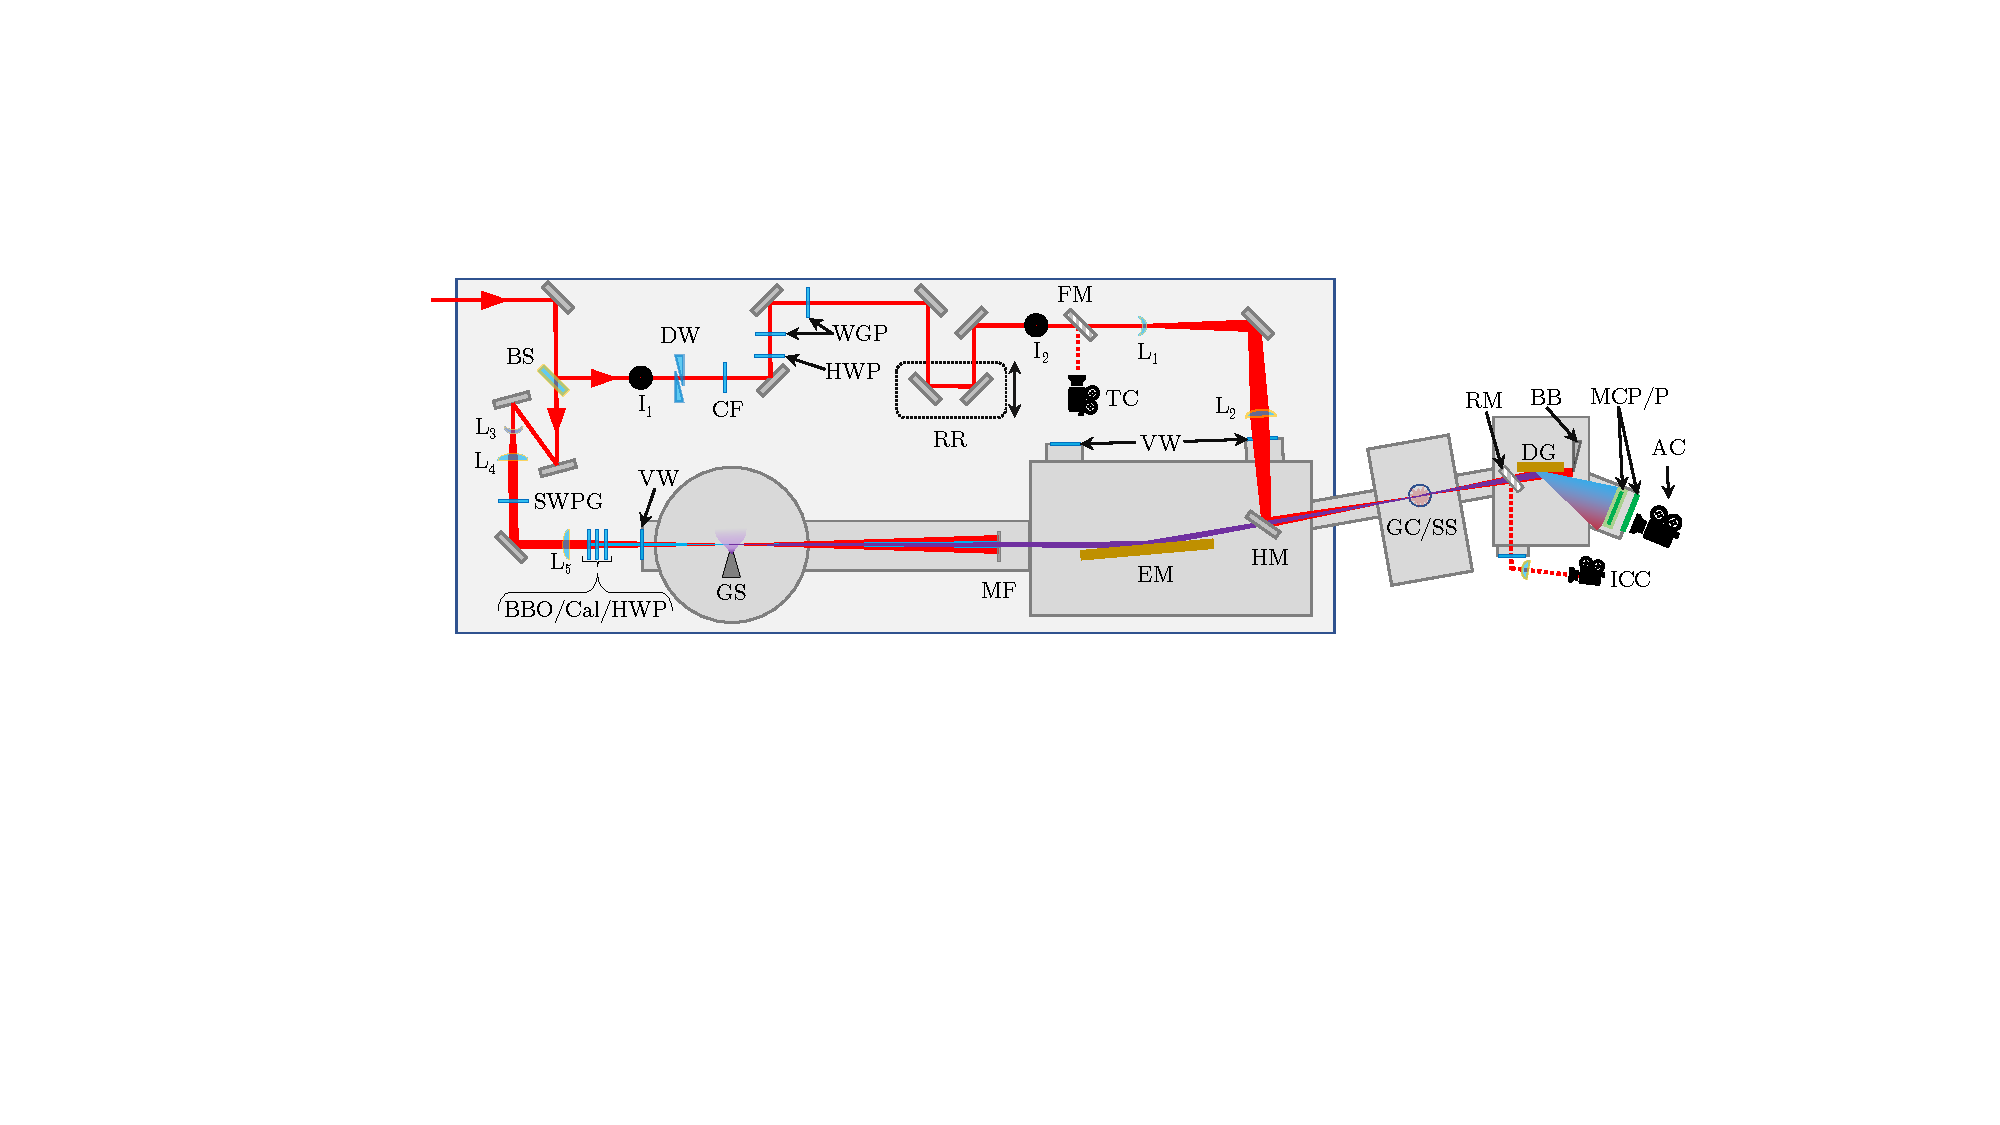
\includegraphics[width=1.0\textwidth]{figures/Beamline/beampath_sketch_3.pdf}
	\caption[Schematic of TABLe optical layout.]{Schematic of the beam path for the TABLe interferometer. The input laser is shown in red, its second harmonic in  blue, and the generated XUV in purple.  \textbf{BS}: Beamsplitter (Thorlabs BSF20-C), \textbf{I$_1$} and \textbf{I$_2$}: Irises used for alignment into interferometer. \textbf{DW}: Delay wedges for fine delay control, see section \ref{sec:delay_wedges}. \textbf{CF}: Color filter to remove parasitic colors from TOPAS (Thorlabs FELH1000). \textbf{HWP}: Half-wave plate. \textbf{WGP}: Wire grid polarizer. \textbf{RR}: Retro reflector for coarse delay adjustment.  \textbf{FM}: Flip mirror. \textbf{TC}: Thermal camera used for alignment.  \textbf{L$_1$}: $f=-300$ mm lens (Thorlabs LF1015-C). \textbf{L$_2$}: $f=500$ mm lens (Thorlabs LA1380-C). \textbf{VW}: Vacuum window, 3 mm CaF$_2$, \textbf{HM}: Hole mirror with 10 mm hole.  \textbf{L$_3$}: $f=-400$ mm lens.  \textbf{L$_4$}: $f=500$ mm lens. \textbf{SWPG}: Square-wave phase grating. \textbf{L$_5$}: $f=400$ mm lens.  \textbf{BBO}: Second-harmonic generation crystal.  \textbf{Ca}l: Calcite. \textbf{GS}: Gas source for HHG. \textbf{MF}: Metallic filter. \textbf{EM}: Ellipsoidal mirror. \textbf{GC/SS}: Gas cell or solid sample. \textbf{RM}: Removable mirror for \textit{in-situ} diagnostics.    \textbf{ICC}: camera for \textit{in-situ} diagnostics. \textbf{DG}: VLS diffraction grating. \textbf{BB}: Baffles to block zero order diffraction.  \textbf{MCP/P}: Microchannel plate and phosphor.  \textbf{AC}: Andor Neo 5.5 CMOS camera.}
	\label{fig:beampath_sketch}
\end{sidewaysfigure}


\subsection{Time Delay Control}
\label{sec:delay_wedges}

An important consideration in pump/probe experiments is how to control the delay between the pump and probe pulses.  To control this delay, there are typically two methods that can be employed optically.  The first to to use a retro-reflector that is mounted on a motorized stage \cite{jagerAttosecondTransientAbsorption2018, jagerAttosecondTransientAbsorption2017, bellTransientAbsorptionSpectroscopy2013, jiangChargeCarrierDynamics2015, borjaElectronDynamicsSolids2016, chengAttoseondTransientAbsorption2015}.  With this method, the delay is simply related to the displacement of the motorized stage by the relationship $\Delta\tau = 2\Delta x/c$.  This means that a displacement of 10 nm by the motorized stage would lead to a delay of 67 as, whereas a displacement of 2 in. would lead to a delay of 339 ps. This setup is advantageous if large delays are required (10s of ps to a few ns), however for the short time steps that are required for an attosecond measurement (typically on the order of 100 as) the mechanical requirements on the motor being used to move the retro are very high.  Since a 100 as step would equate to a translation of 15nm, this would require the use of a piezoelectric motor.  Piezo motors and their associated electronics tend to be expensive, and they have inherent problems because they exhibit nonlinear movement due to hysteresis and they tend to drift and creep after actuation.  This can be abated through a feedback sensor and operating it in a closed-loop mode, however the quality of the sensor and electronics determines how effectively these problems are minimized.

\begin{figure}
	\centering
	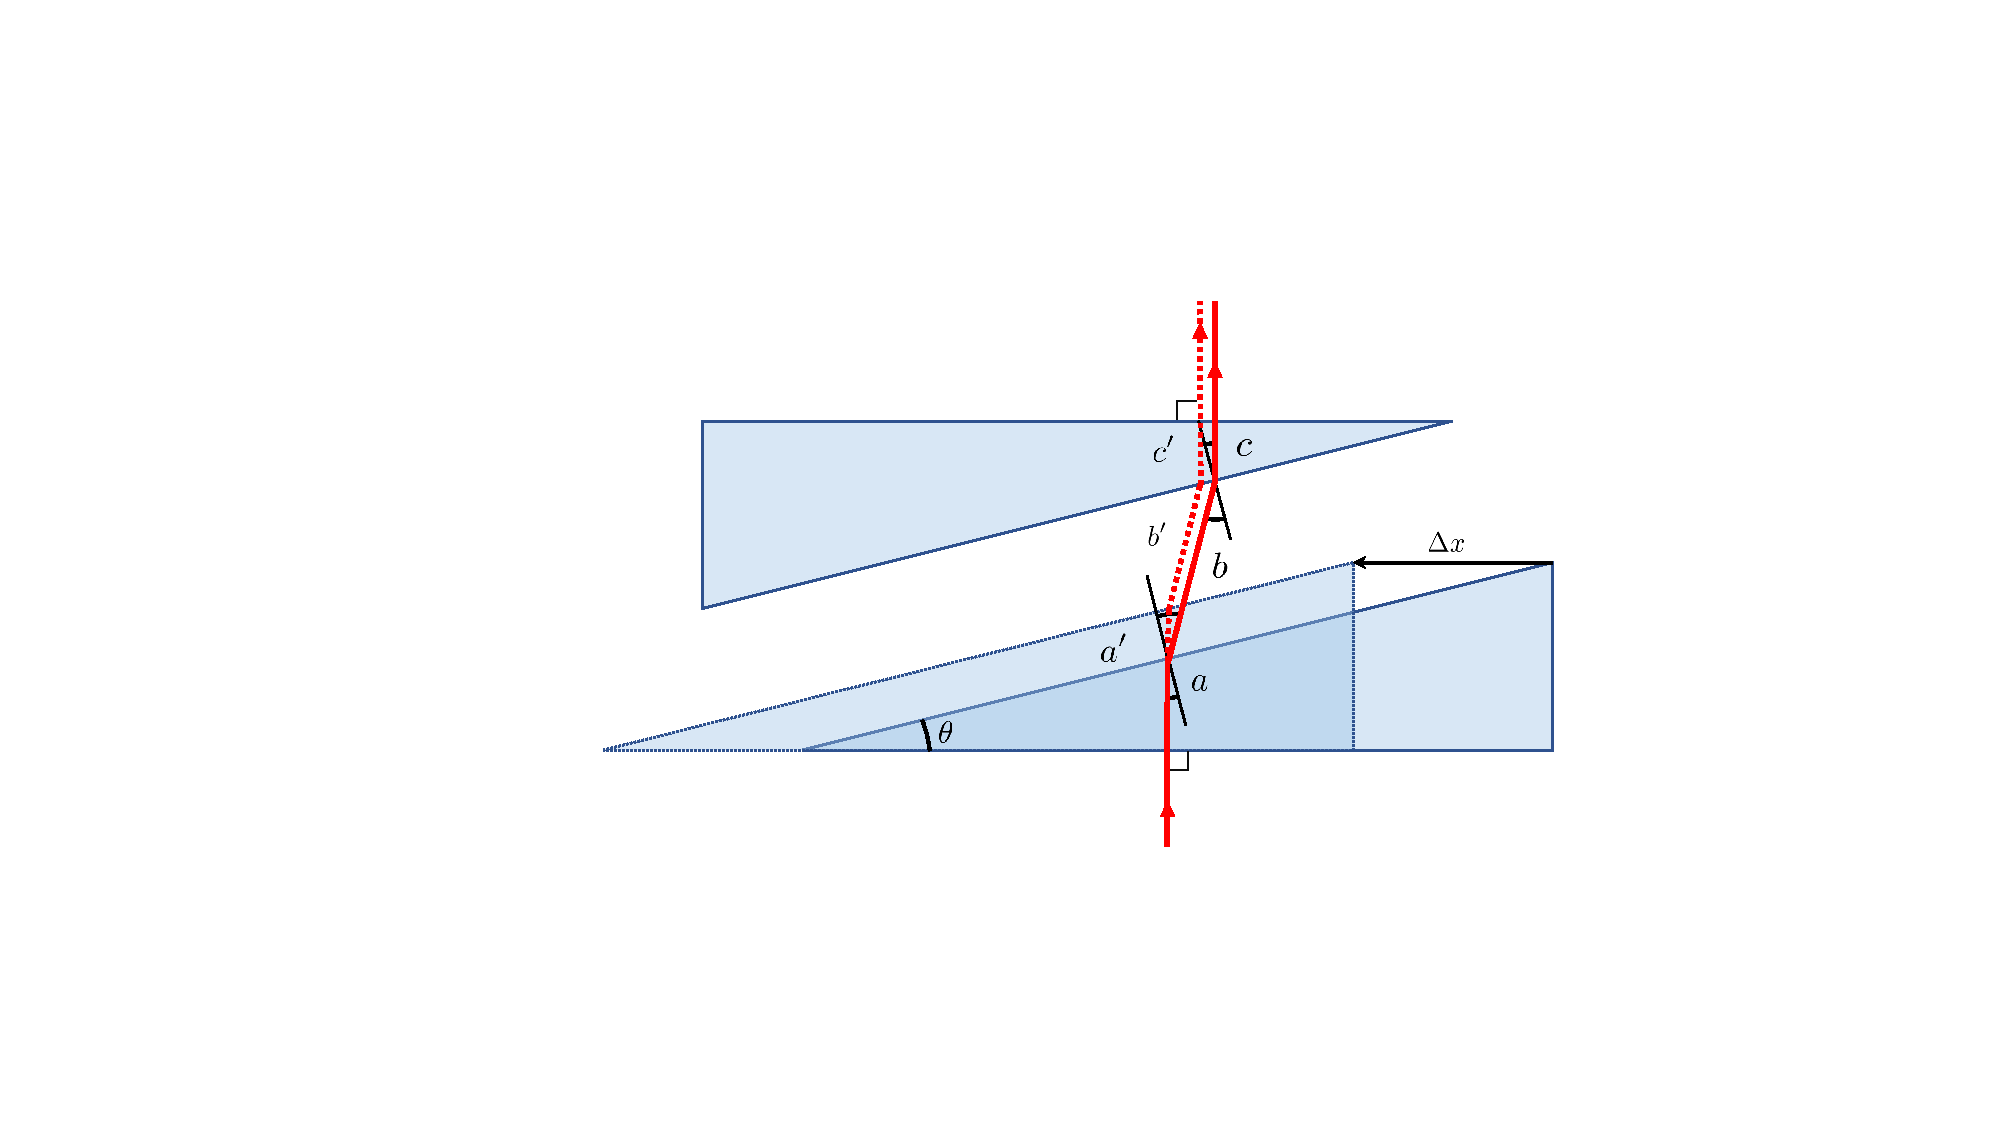
\includegraphics[width=0.6\textwidth]{figures/Beamline/wedge_delay_calibration.pdf}
	\caption[Schematic of FS wedges used for delay control]{Schematic of the FS wedges used to control the time delay between the IR and XUV pulses in the dressing and generation arms interferometer, respectively. The wedges are aligned such that the input beam is normal to the first wedge face, and the beam exits the wedges normal to the last face of the second wedge.  Only one of the wedges is motorized and is shown before and after a displacement by an amount $\Delta x$.}
	\label{fig:wedges}
\end{figure}

The second common method to control the delay between the pump and probe pulse is to use a pair of glass wedges \cite{chirlaAttosecondPulseGeneration2011, gormanAttosecondProbingElectron2018, kiesewetterDynamicsNearThresholdAttosecond2019}. A schematic of how this is achieved is shown in figure \ref{fig:wedges}.  In this scheme, only one of the glass wedges is motorized, and the direction of translation is perpendicular to the input beam and parallel to the first glass face.  The path that a ray would take through the wedge pair is shown before ($a\rightarrow b\rightarrow c$) and after ($a' \rightarrow b'\rightarrow c'$) translation by an amount $\Delta x$.  Assuming that the wedge angle is $\theta$, the path after translation by $\Delta x$ can be written as
\begin{align}
\label{eqn:path_lengths}
	a'&=a+\Delta x \tan\theta\\
	b'&=b-\Delta x \bigg(\frac{\sin\theta}{\cos\psi}\bigg)\\
	c'&=c+\Delta x \tan\theta\bigg(\frac{\sin(\psi-\theta)}{\cos\theta}\bigg)
\end{align}
where
\begin{equation}
	\psi = \arcsin(n\sin\theta)
\end{equation}
is given by Snell's Law \cite{pedrottiIntroductionOptics2007}. From the difference in optical path length between these two paths, one can calculate the time delay $\Delta\tau$ introduced by a translation of $\Delta x$, and this relationship is given by
\begin{equation}
\label{eqn:time_delay}
	\Delta\tau = \frac{\Delta x}{c}\Bigg[n\tan\theta - \frac{\sin\theta}{\cos\psi}-n\tan\theta\bigg(\frac{\sin(\psi-\theta)}{\cos\theta}\bigg)\Bigg].
\end{equation}
For a pair wedges made out of fused silica (Infrasil) with a wedge angle of $\theta=4^\circ$ and a beam of wavelength 1430 nm (n=1.4454), equation \ref{eqn:time_delay} becomes
\begin{equation}
\label{eqn:numerical_relationship_wedges}
	\Delta\tau = \Bigg(102 \bigg[\frac{\mathrm{as}}{\mathrm{\mu m}}\bigg]\Bigg)\Delta x.
\end{equation}
This entails that a translation of 1 $\mu$m would lead to a delay of only 100 as.  This reduction in motor step to delay step ratio compared to the retroreflector case means that the requirements on the motorized stage are greatly reduced.  Additionally, since the glass wedges are a transmissive optic, they are inherently less sensitive to vibrations when compared to a retroreflector.

In the TABLe apparatus, both types of delay control have been implemented, as shown in figure \ref{fig:beampath_sketch}.  The retroreflector is mounted on a translation stage with 2 inches of travel that is controlled manually with a micrometer.  The primary use for the retroreflector is to make coarse adjustments to the dressing arm to account for changes in temporal overlap between the two arms of the interferometer.  Typically, this is due to adjustments made to the interferometer itself (such as introducing new optics) or due to changes in the input laser, usually either pointing or wavelength.  

To finely control the delay, a pair of glass wedges is used.  These wedges are made out of fused silica, and have a wedge angle of $\theta=4^\circ$.  The first of the two wedges are motorized in manner similar to that shown in figure \ref{fig:wedges}.  The stage that the first wedge is mounted to has a total travel of 1 inch, and it is controlled by a Thorlabs Z825B DC servo motor.  This "pencil" motor, as it is known in the lab, has a minimum repeatable incremental motion of 0.2 $\mu$m and is encoded, so it's absolute position is known to within the homing accuracy of $\pm1$ $\mu$m.  From equation \ref{eqn:numerical_relationship_wedges}, using these wedges at 1430 nm with a step size of 1 $\mu$m will give a delay of 101 as.


\subsection{IR Dressing Intensity}
\label{sec:dressing_intensity}

An important consideration in any pump/probe experiment is the intensity of the IR field that is used as a probe/dressing field. Ideally, one would like to be able to control the intensity such that both perturbative and strong-field regimes can be accessed with the same optical setup.  This can be achieved by selecting an optical setup that has a high peak intensity and then attenuate the beam to achieve a lower intensity.  Attenuation can be achieved through the use of neutral density (ND) filters, however they can lead to several complications.  Since the ND filter would be placed in only one arm of the interferometer to control only the dressing intensity, any variation in thickness between different ND filters would lead to a change in temporal overlap.  Additionally, any change in positioning when switching ND filters will lead to a slight change in spatial overlap. In light of this, the method to attenuate the beam that was implemented in the TABLe interferometer is a half-wave plate (HWP) and a wire grid polarizer (WGP).  By rotating the polarization using the HWP, we can finely control the intensity  of the dressing field by using the WGP to transmit only one component of the rotated polarization.  The WGP is set such that the initial polarization is maintained, and this insures that the polarization of the IR and XUV are parallel in the interaction region.  A second WGP is used to increase the effective extinction ratio to ensure that the field is linearly polarized even when it is being strongly attenuated.  The extinction ratio of one of the WGP (Thorlabs WP25M-UB) is approximately 12500:1 at 1430 nm.  Using this setup in conjunction with a beam splitter that reflects 8\% of the input energy to the dressing arm, the pulse energy can be tuned between 1 $\mu$J and 125 $\mu$J.

\begin{figure}
	\centering
	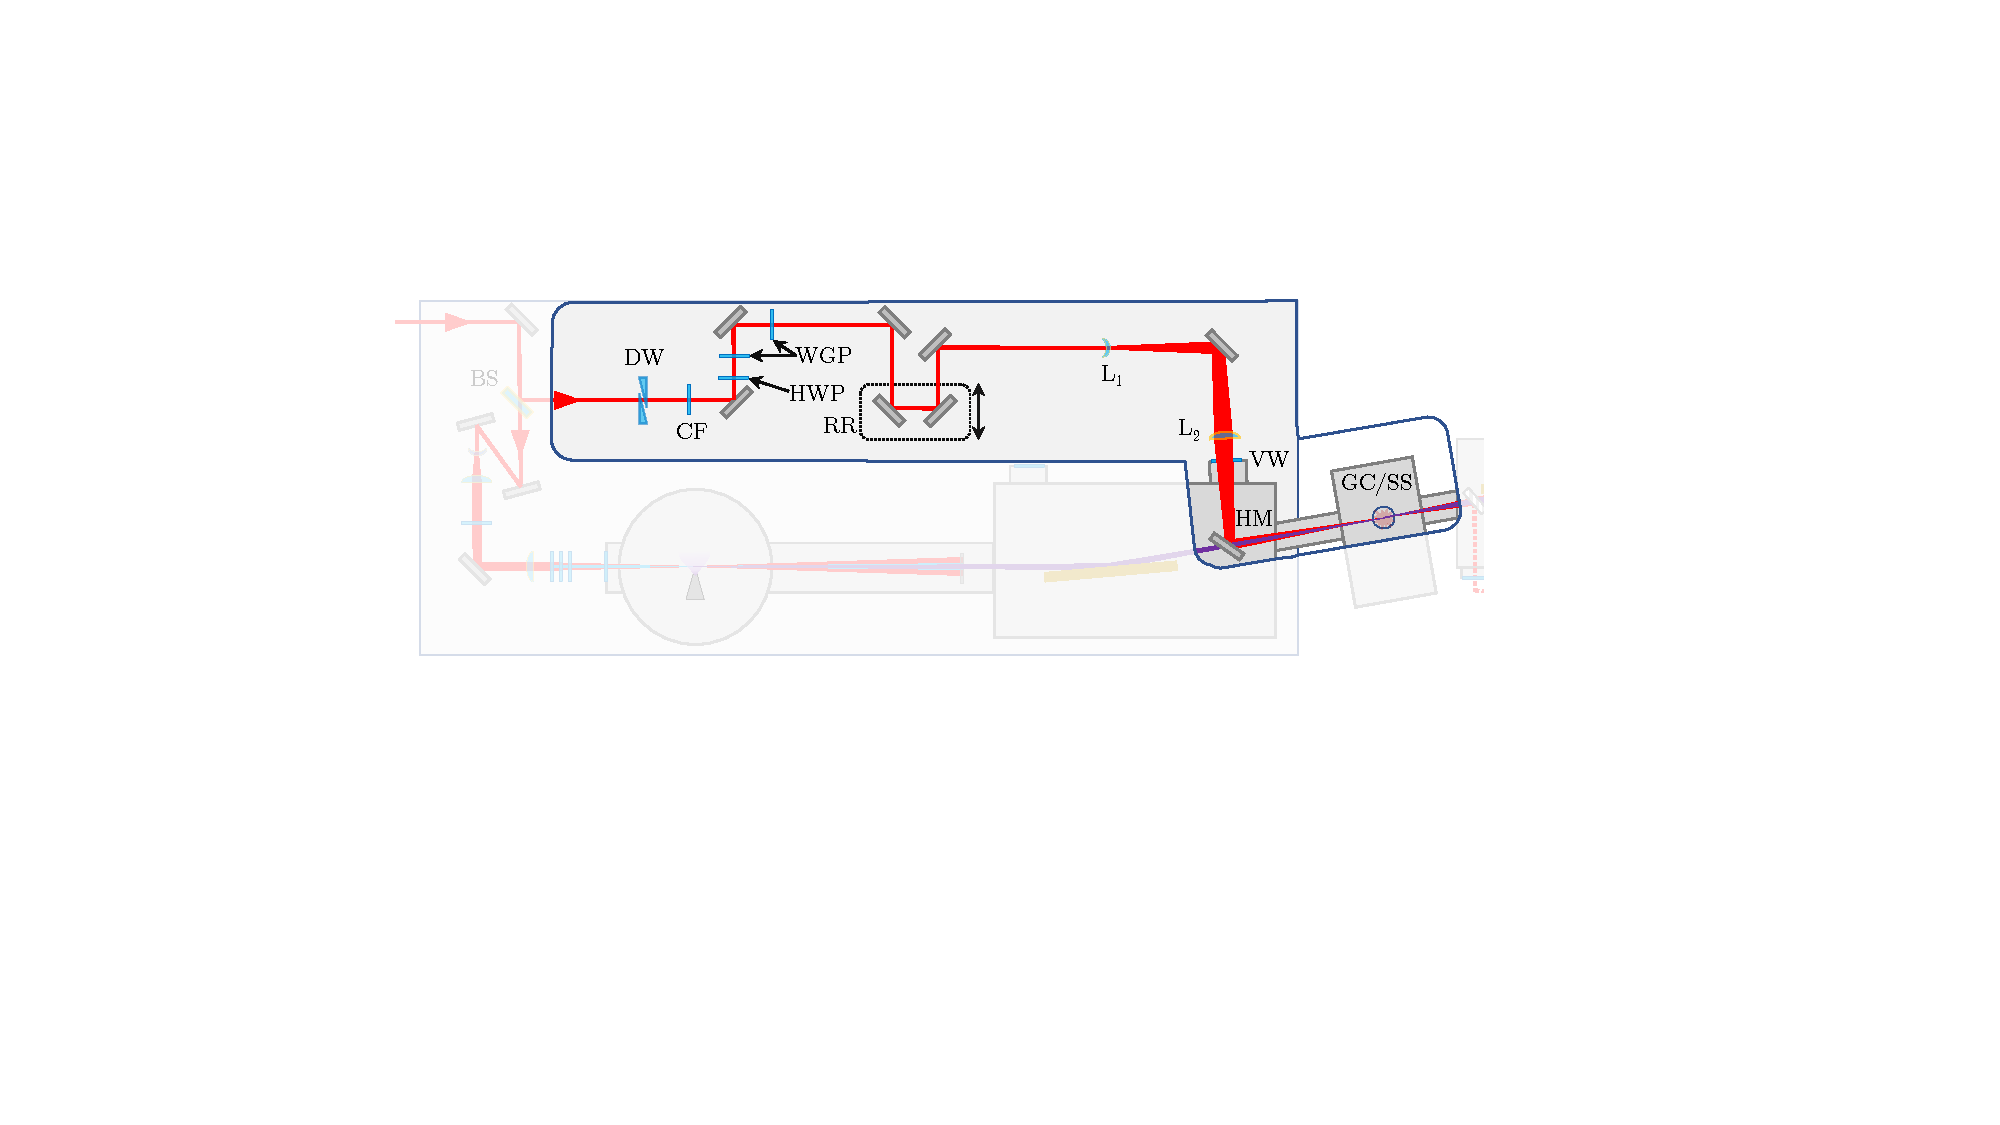
\includegraphics[width=0.9\textwidth]{figures/Beamline/dressing_arm.pdf}
	\caption[Optical layout of dressing arm]{Optical layout of the dressing arm of the TABLe interferometer. HWP and WGP are used to finely control the power in the dressing arm.  The lenses L$_1$ and L$_2$ were chosen to achieve a high intensity at the focal plane in the target chamber.  This was done to have the capability to drive strong-field processes in a gas medium \cite{kiesewetterDynamicsNearThresholdAttosecond2019}.  See figure \ref{fig:beampath_sketch} for full details of the interferometer.}
	\label{fig:dressing_arm}
\end{figure}

The next design consideration for the dressing arm of the interferometer is choosing focusing optics to set the peak intensity that is achievable at the interaction region.  The two main options in this regard are either focusing mirrors or lenses.  Focusing mirrors have a significant advantage in the fact that they are achromatic, however their use leads to an optical system that is generally larger in optical path length and is difficult to switch between focal geometries. Lenses in that regard are well suited to adjusting between different experimental configurations without changing the overall footprint of the interferometer.  The dressing lenses that are used in all of the experiments in this dissertation are shown in \ref{fig:dressing_arm}, and they were originally selected to achieve the highest possible intensity at the focal plane given the geometrical constraints of the TABLe \cite{kiesewetterDynamicsNearThresholdAttosecond2019}. This choice of lenses was made to drive strong-field processes in rare gas atoms in the interaction region, and they were selected based upon calculations done by D. Kiesewetter using a hole mirrors as both beam splitters in the interferometer \cite{kiesewetterDynamicsNearThresholdAttosecond2019}. His calculations estimated that the peak intensity at 1300 nm was 0.59 TW/cm$^2$ for a pulse energy of 1 $\mu$J just before L$_1$ in figure \ref{fig:dressing_arm}.

\begin{sidewaysfigure}%[ht]
	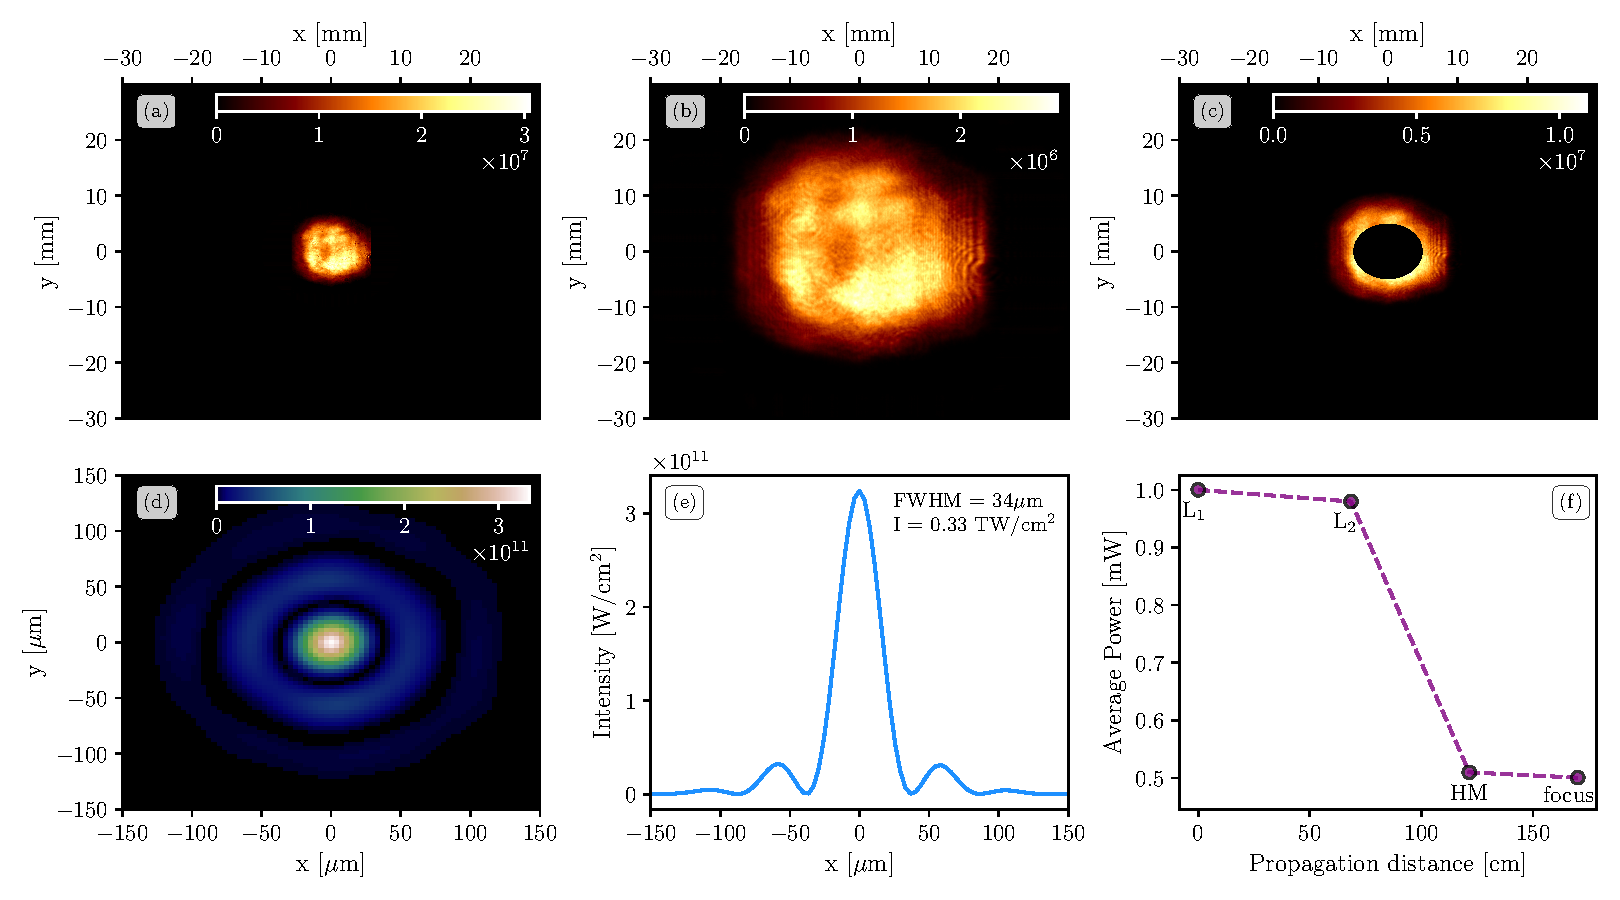
\includegraphics[width=\textwidth]{figures/Beamline/pump_intensity_profiles_1430nm_1uj.pdf}
	\caption[Calculation of dressing intensity]{(a) Beam profile of the signal from the TOPAS pumped by the Spitfire laser system.  Wavelength is 1430 nm and the pulse is normalized to 1 $\mu$J of pulse energy.  Beam profile was measured using a thermal camera, and is used as the input to the beam propagation simulation that is initiated just before L$_1$ in figure \ref{fig:dressing_arm}. (b) Numerically propagated beam profile just after L$_2$ in figure \ref{fig:dressing_arm}. (c) Beam profile just after reflecting off the hole mirror.  (d) Calculated intensity profile at the focal plane in the interaction region. (d) Lineout of the calculated intensity profile.  For an input pulse energy of 1 $\mu$J, a peak intensity of 0.33 TW/cm$^2$ can be achieved.  (f) Integrated average power at different point in the calculation.  The main source of energy loss is due to the hole mirror, which only reflects 52\% of the incident light.  The hole mirror has an inner radius of 5 mm in this case.}
	\label{fig:dressing_intensity}
\end{sidewaysfigure}


For the experiments described herein, the initial beam splitter was changed to a beam sampler, and the recombining hole mirror was changed to a hole diameter of 10 mm from 6 mm.  This was done to maximize the XUV flux by sending as much energy to generation as possible while minimizing clipping of the XUV with the hole mirror.  In light of these changes, it is important to determine what the new peak intensity is at the focus.  To accurately determine the intensity, a beam propagation simulation is performed using the measured beam profile.  It is important to use the measured beam profile because the spatial mode out of the TOPAS is decidedly non-Gaussian, and this can be seen in figure \ref{fig:dressing_intensity} (a) which shows the beam profile at 1430 nm measured on a thermal camera.  Beam propagation is implemented using an open-source Python package developed by Flexible Optical B.V. (OKO Tech) called LightPipes.  The package consists of numerical methods to calculate the Fresnel integral
\begin{equation}
\label{fresnel_integral_0}
u(x,y,z)=\frac{i k}{2\pi z}e^{i k z}e^{i k (x^2+y^2)/2z}\int_{-\infty}^{\infty}\int_{-\infty}^{\infty}u(\xi,\eta,0) e^{ik(\xi^{2}+\eta^{2})/2z} e^{-ik(x\xi + y\eta)/z} \diff\xi\diff\eta
\end{equation}
which gives the field $u(x,y,z)$ after propagation of a distance $z$, given an initial field profile of $u(x,y,0)$.  Using this formalism, a thin lens of focal length can be treated as adding a quadratic phase $\phi=-\pi(x^2+y^2)/\lambda f$ to the field, and the effect of apertures can also be included to account for the effect of diffraction on the beam profile and intensity \cite{goodmanIntroductionFourierOptics2005}.

The results of the simulation are shown in figure \ref{fig:dressing_intensity}.  This simulation was performed for an input pulse energy of 1 $\mu$J at a wavelength of 1430 nm. The simulation begins just before L$_1$ in \ref{fig:dressing_arm} and the beam is propagated through to the interaction region GC/SS.  The beam profile at L$_2$ and immediately after the hole mirror is shown in figure \ref{fig:dressing_intensity} (b) and (c), and the intensity profile at the focus is shown in figure \ref{fig:dressing_intensity} (d).  From these simulations, the peak intensity for a pulse energy of 1 $\mu$J is 0.33 TW/cm$^2$. For the range of pulse energies available in the dressing arm, this corresponds to an intensity range of 0.33 - 41.3 TW/cm$^2$ that is achievable.

\subsection{XUV Beam Size}
\label{sec:xuv_beam_size_knife_edge}

Another important consideration in any pump/probe experiment is the beam size of the probe relative to the pump in the interaction region.  The reason for this is because the probe beam inherently samples the excited state of the system induced by the pump at intensities within the intersection of the pump and probe focal volumes contained within the system being studied.  Thus, a smaller probe waist relative to the pump waist means that a narrower distribution of pump intensities will be sampled by the XUV probe.  The width of this distribution limits the ability to study intensity dependent effects, and it is a critical parameter to control. As stated previously, the demagnification of the XUV spot size provided by the ellipsoidal mirror helps tremendously to achieve as small ratio of probe to pump beam sizes even at small pump beam sizes that are used.

Additionally, it is also of great importance to place the sample at the focus of both the XUV and the IR beams in the target chamber.  This can be done easily with the IR either through direct imaging of the beam or by using an intensity dependent effect (such as second harmonic generation from a BBO) to find the peak intensity along the k-direction of the IR beam.  The focus of the XUV is more difficult to find because it must be found in vacuum.  One method to find the focus is to measure the beam diameter at various points along the k-direction of the XUV to find the minimum beam diameter.  A method to do this is to employ a knife-edge measurement \cite{arnaudTechniqueFastMeasurement1971, skinnerMeasurementRadiusHighpower1972,marshallTwoMethodsMeasuring2010,almeidaHarmonicsBeamsCharacterization2016}.

\begin{figure}
	\centering
	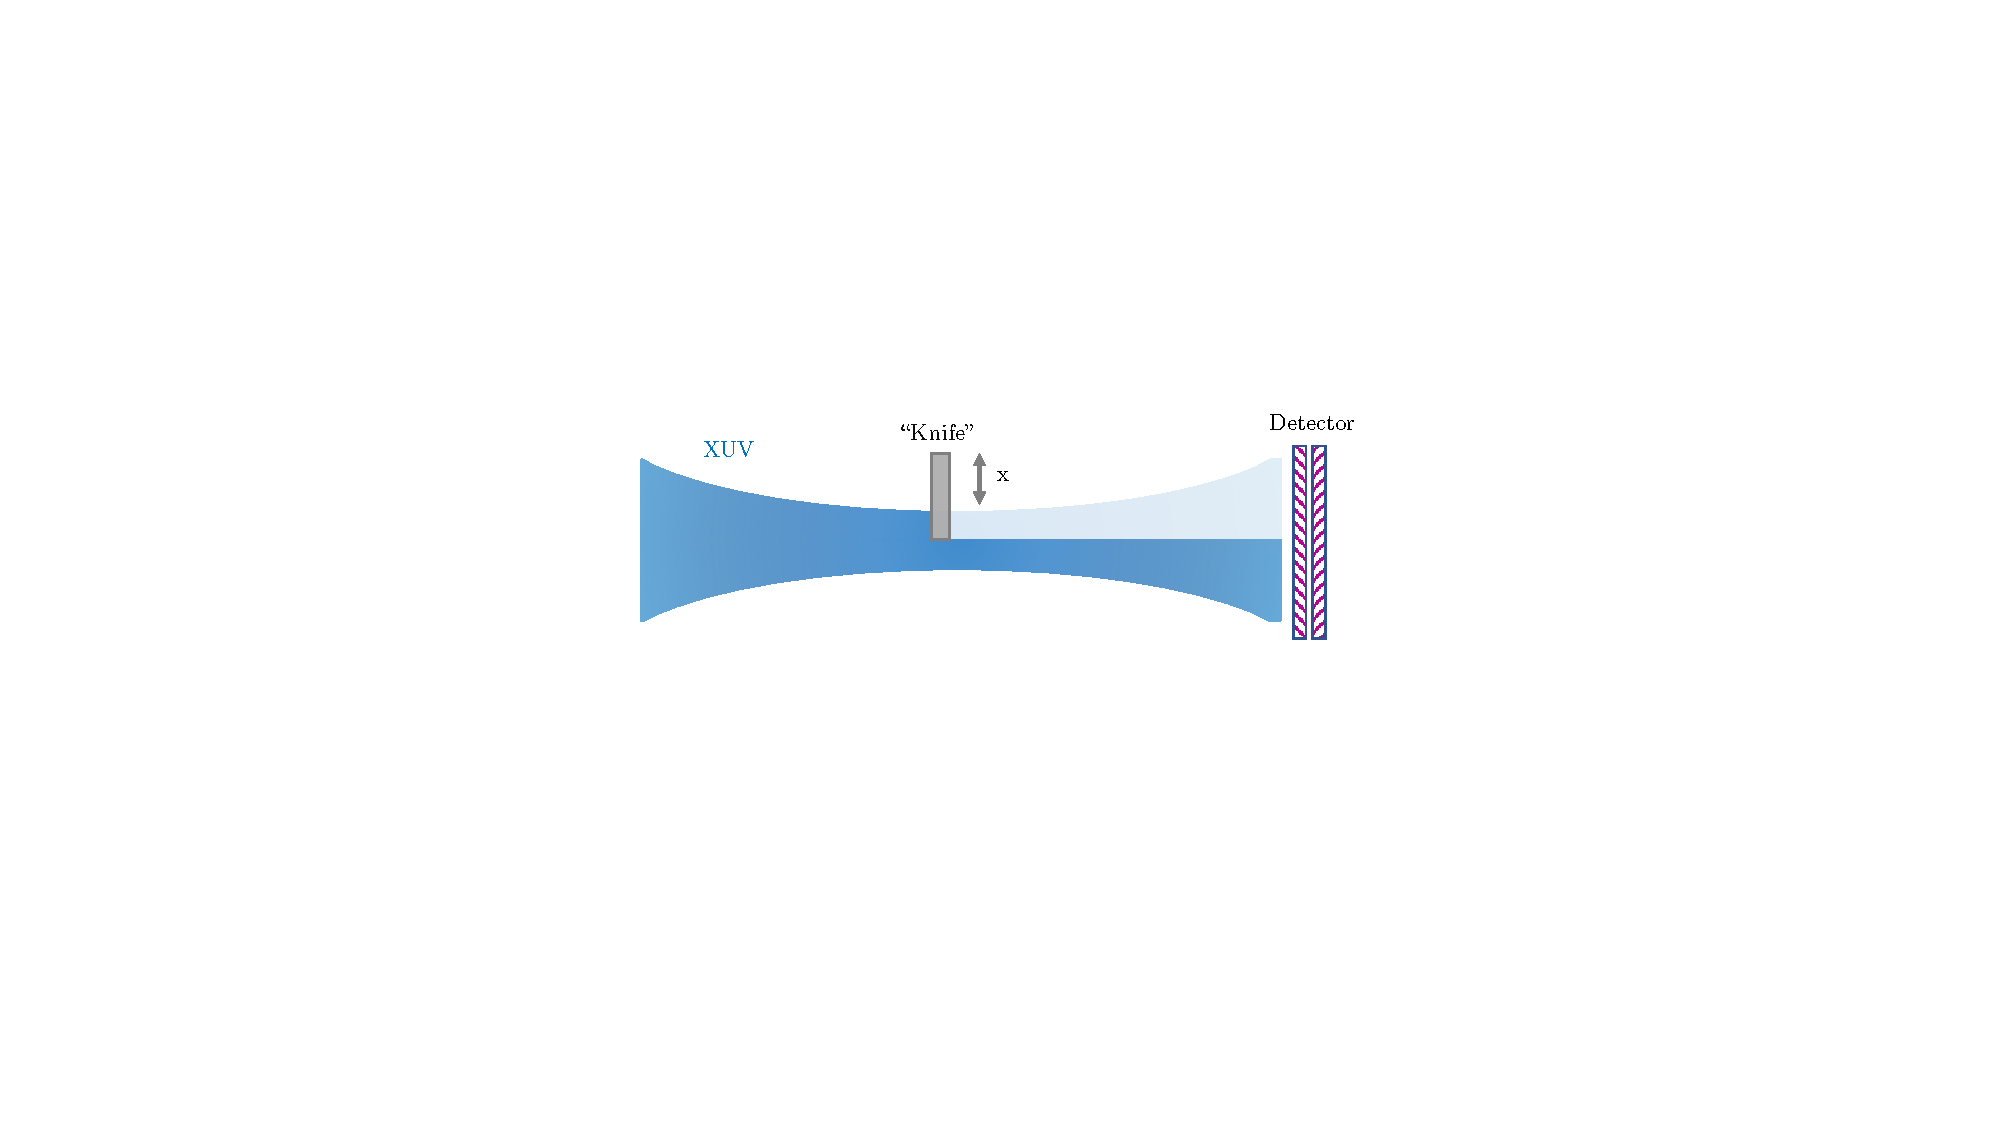
\includegraphics[width=0.7\textwidth]{figures/Beamline/knife_edge_xuv.pdf}
	\caption[Schematic of knife-edge technique to measure beam size]{Schematic of knife-edge technique to measure beam size. By translating a sharp beam block through the focus and measuring the total transmitted power the beam profile can be reconstructed.}
	\label{fig:knife_edge_beam_size_measurement}
\end{figure}

The principle behind the knife-edge measurement is simple, and it is shown schematically in figure \ref{fig:knife_edge_beam_size_measurement}.  In the measurement, a "knife" is translated through the beam to be measured perpendicular to the k-direction of the beam.  The knife is simply an opaque material that has a sharp edge to minimize scattered light.  As this knife is translated through the focus, the total power is measured further downstream as a function of the knife's position within the beam, and this dependence is given by
\begin{equation}
	\label{eqn:knife_edge_power}
	P(x,z) = \int_{-\infty}^{\infty}\int_{-\infty}^{x}I(x', y',z)\diff y\diff x'
\end{equation} 
where $I(x,y,z)$ is the intensity of the beam.  For a Gaussian beam, this relationship becomes
\begin{equation}
	\label{eqn:knife_edge_power_guassian}
	P(x,z) = \frac{P_0}{2}\mathrm{erfc}\bigg(\frac{x\sqrt{2}}{w(z)}\bigg)
\end{equation}
where $w(z)$ is waist radius as a function of $z$ and is given by
\begin{equation}
	\label{eqn:gaussian_waist_radius}
	w(z)=w_0\sqrt{1+\bigg(\frac{z - z_0}{z_R}\bigg)^2}
\end{equation}
where $z_R=\pi w_0^2 n/\lambda$ is the Rayleigh range and $z_0$ is the position of the focus along the k-direction. 

An example of this technique being used to measure the beam size of the XUV is shown in figure \ref{fig:xuv_beam_size}.  In this case, the knife being used is the beveled edge of a silicon frame that is 300 $\mu$m thick. The thickness of the frame is such that the transmission is negligible through the frame itself.  The integrated harmonic signal is fit to
\begin{equation}
	P(x) = \frac{a}{2}\mathrm{erfc}\bigg(\frac{\sqrt{2}(x-x_0)}{w}\bigg) + b,
\end{equation}
and the beam size can be extracted from the fit.  In this case the beam size was 9 $\mu$m at this position of the XUV focus.  Comparing this beam size to the predicted beam size of the IR, we can see that the XUV spot size relative to the IR spot size is roughly three times smaller.

\begin{figure}
	\centering
	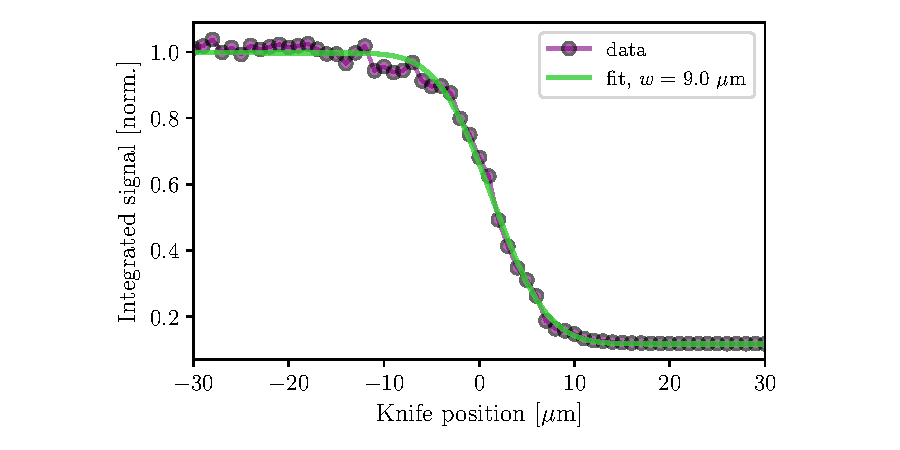
\includegraphics[width=0.9\textwidth]{figures/Beamline/integrated_knife_edge_xuv.pdf}
	\caption[Schematic of knife-edge technique to measure beam size]{Schematic of knife-edge technique to measure beam size. By translating a sharp beam block through the focus and measuring the total transmitted power the beam profile can be reconstructed.}
	\label{fig:xuv_beam_size}
\end{figure}


This measurement can repeated along the k-direction of the XUV beam, and the focus can be mapped out.  An example of this type of measurement is shown in figure \ref{fig:xuv_focus}.  As can be seen, the fit to a Gaussian agrees quite well with the measure dependence of the beam profile.  The extracted Rayleigh range is 1.1 mm with a waist of 6.1 $\mu$m at a motor position of 12.7 mm along the k-direction.  This type of measurement is performed whenever the optical setup is changed in the generation arm of the interferometer, as it insures that the sample is always at the focus of the XUV.
\begin{figure}
	\centering
	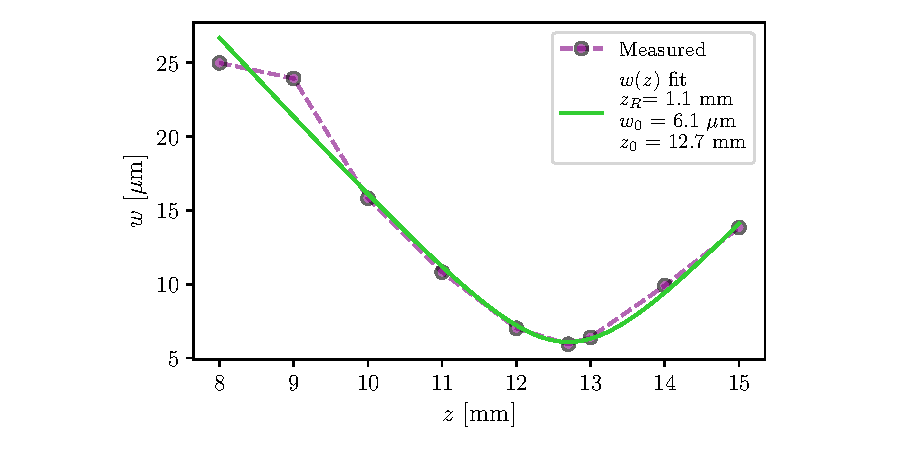
\includegraphics[width=0.9\textwidth]{figures/Beamline/xuv_focus.pdf}
	\caption[Finding focus of XUV using knife-edge measurements]{Focus of the XUV measured using knife-edge method at various points along the k-direction of the XUV beam.}
	\label{fig:xuv_focus}
\end{figure}


\section{Conclusion}

In this chapter the design and optical layout of the Transient Absorption Beamline (TABLe) was described.  This experimental apparatus represent the culmination of years of design, construction, and validation performed by Greg Smith and myself.  The unique capabilities of the TABLe enabled the work detailed in this dissertation to be performed, as well as other experiments \cite{kiesewetterDynamicsNearThresholdAttosecond2019, camperHighRelativephasePrecision2019, leshchenkoHighpowerFewcycleCr2020}.
%\section{Spectrometer Calibration}
%\label{subsec:spec_calibration}

%\begin{figure}
%	\centering
%	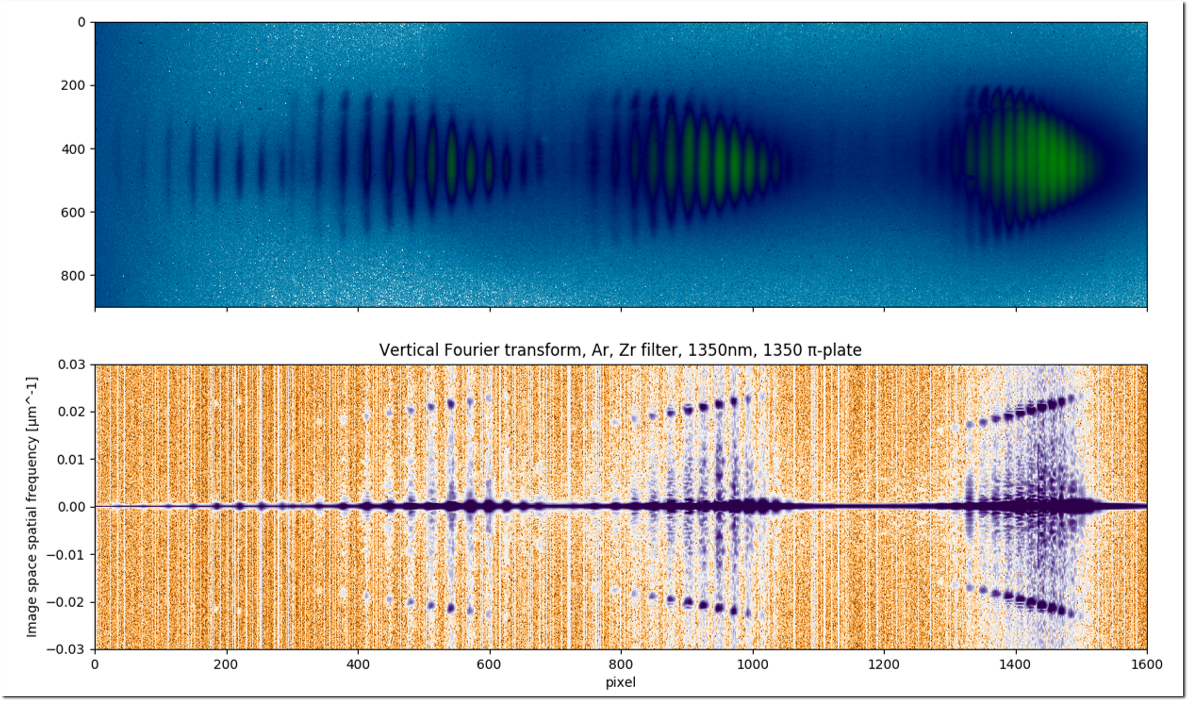
\includegraphics[width=0.9\textwidth]{figures/Beamline/first_to_third_order_diffraction.png}
%	\caption{INCOMPLETE: multiple diffraction orders}
%	\label{fig:first_to_thirds_order}
%\end{figure}

%\begin{figure}
%	\centering
%	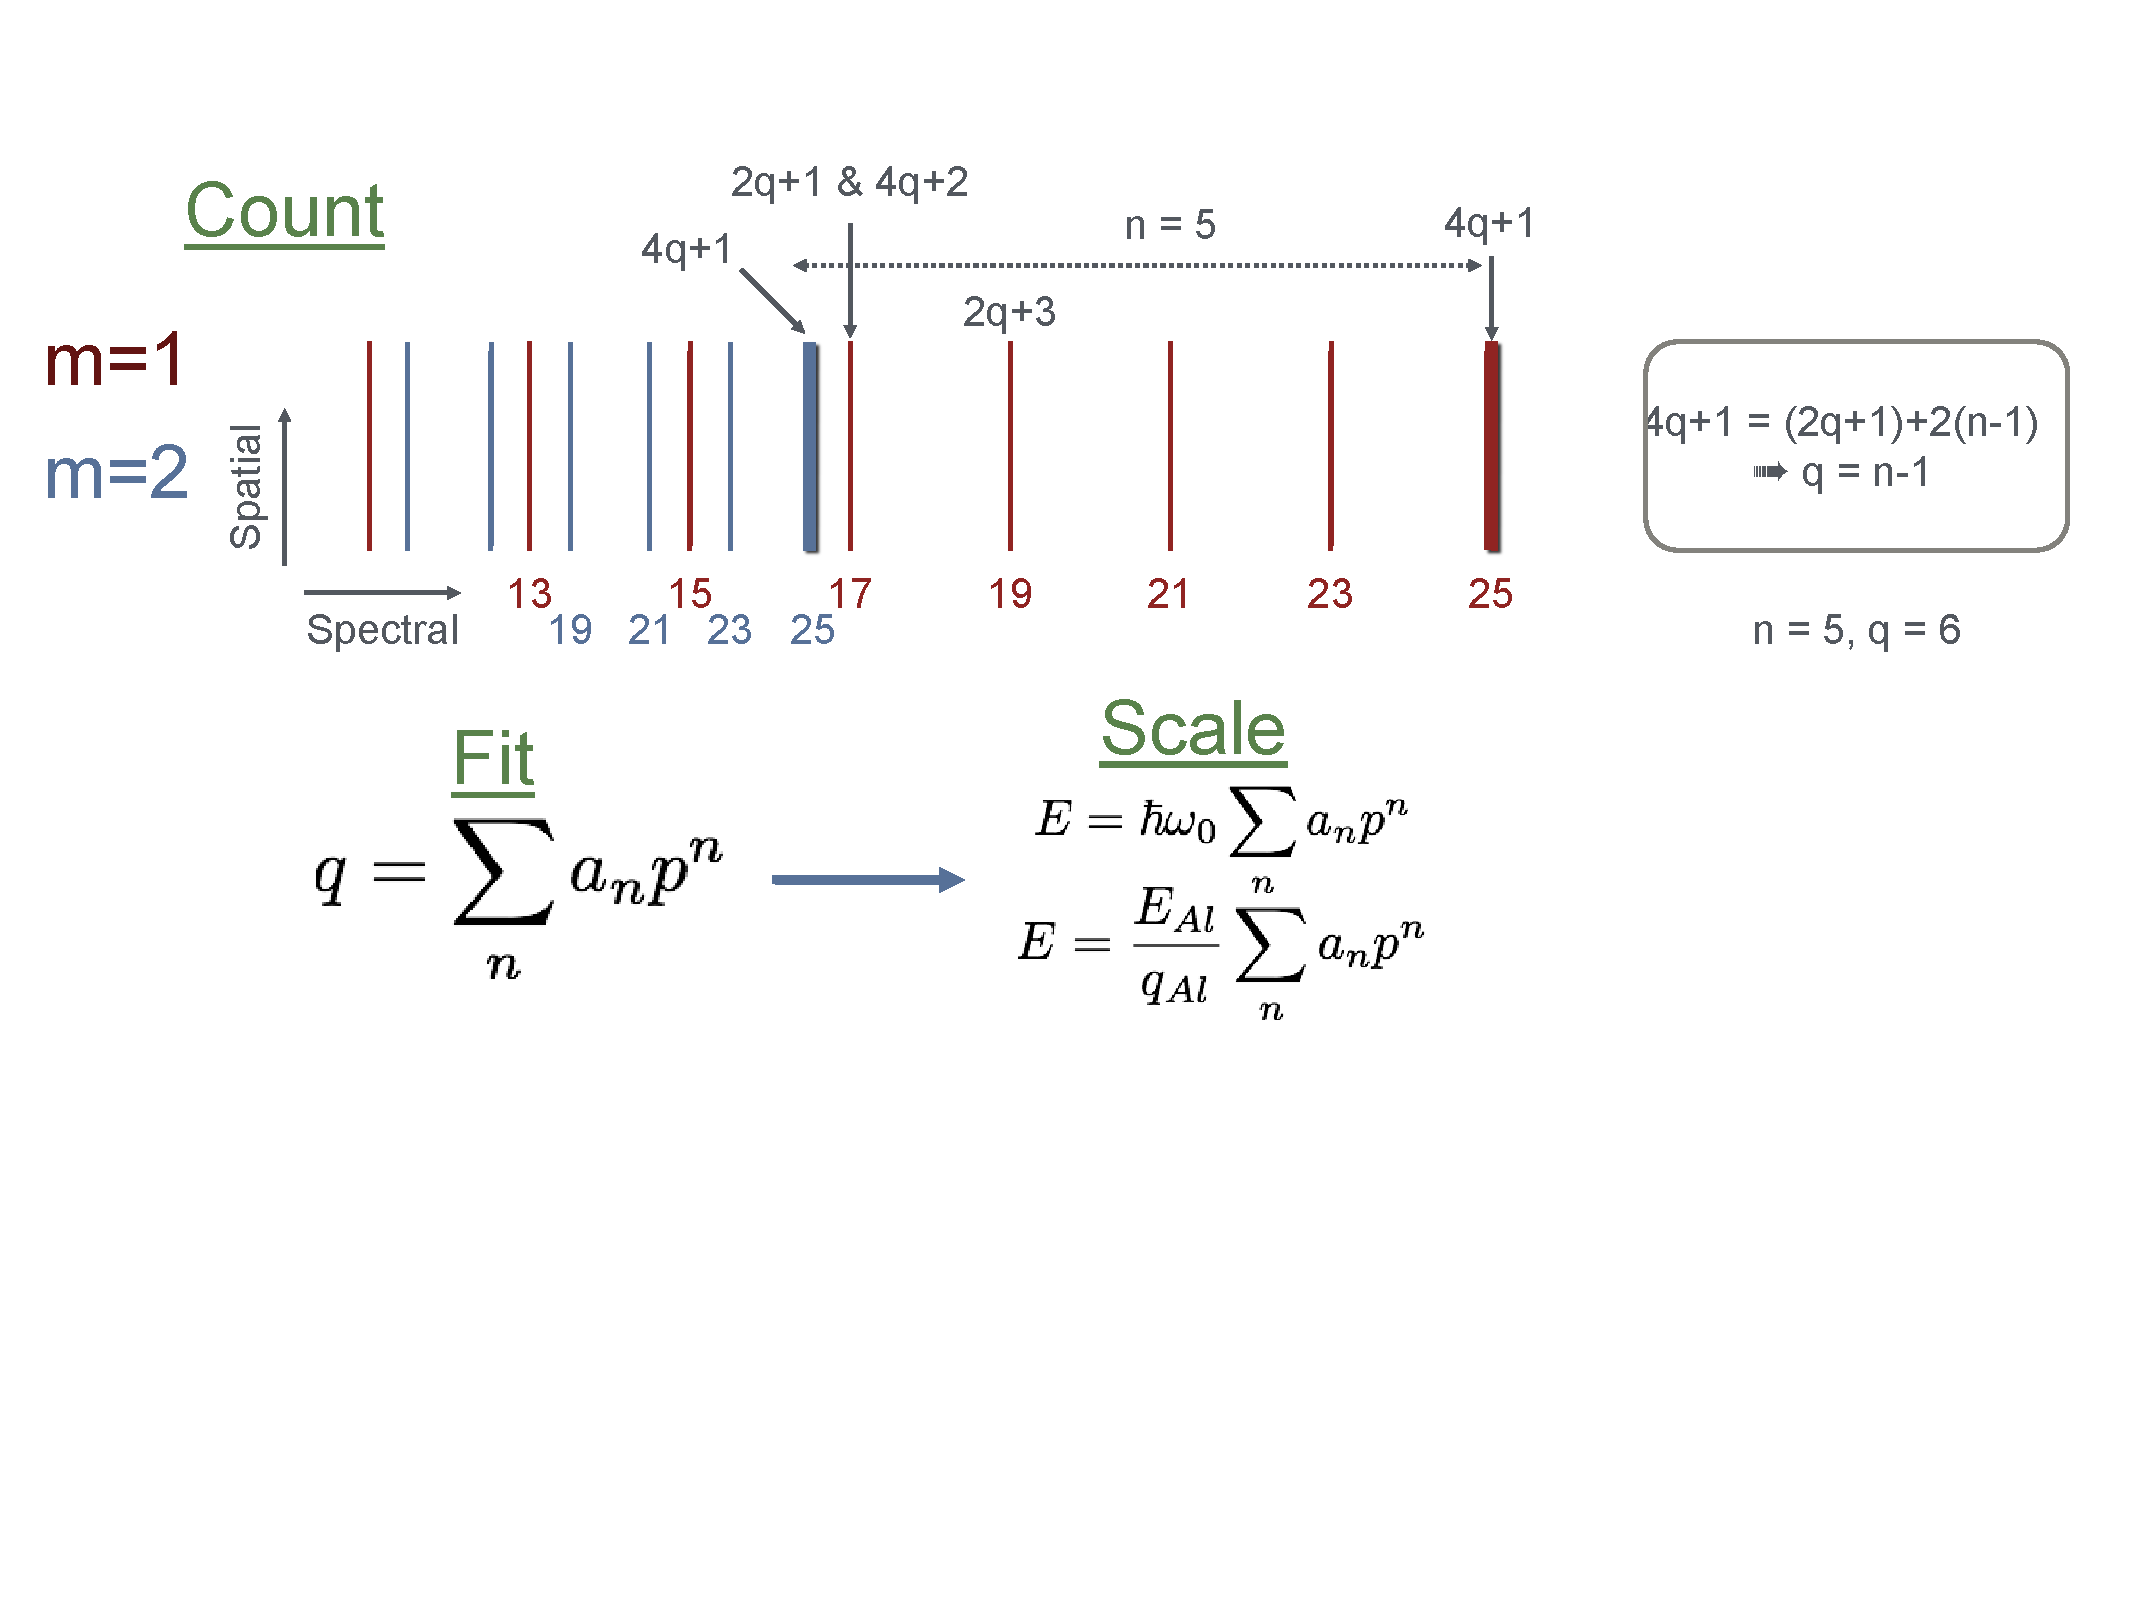
\includegraphics[width=0.9\textwidth]{figures/Beamline/Count_Fit_Scale.pdf}
%	\caption{INCOMPLETE: count fit scale scheme}
%	\label{fig:count_fit_scale_scheme}
%\end{figure}

%\begin{figure}
%	\centering
%	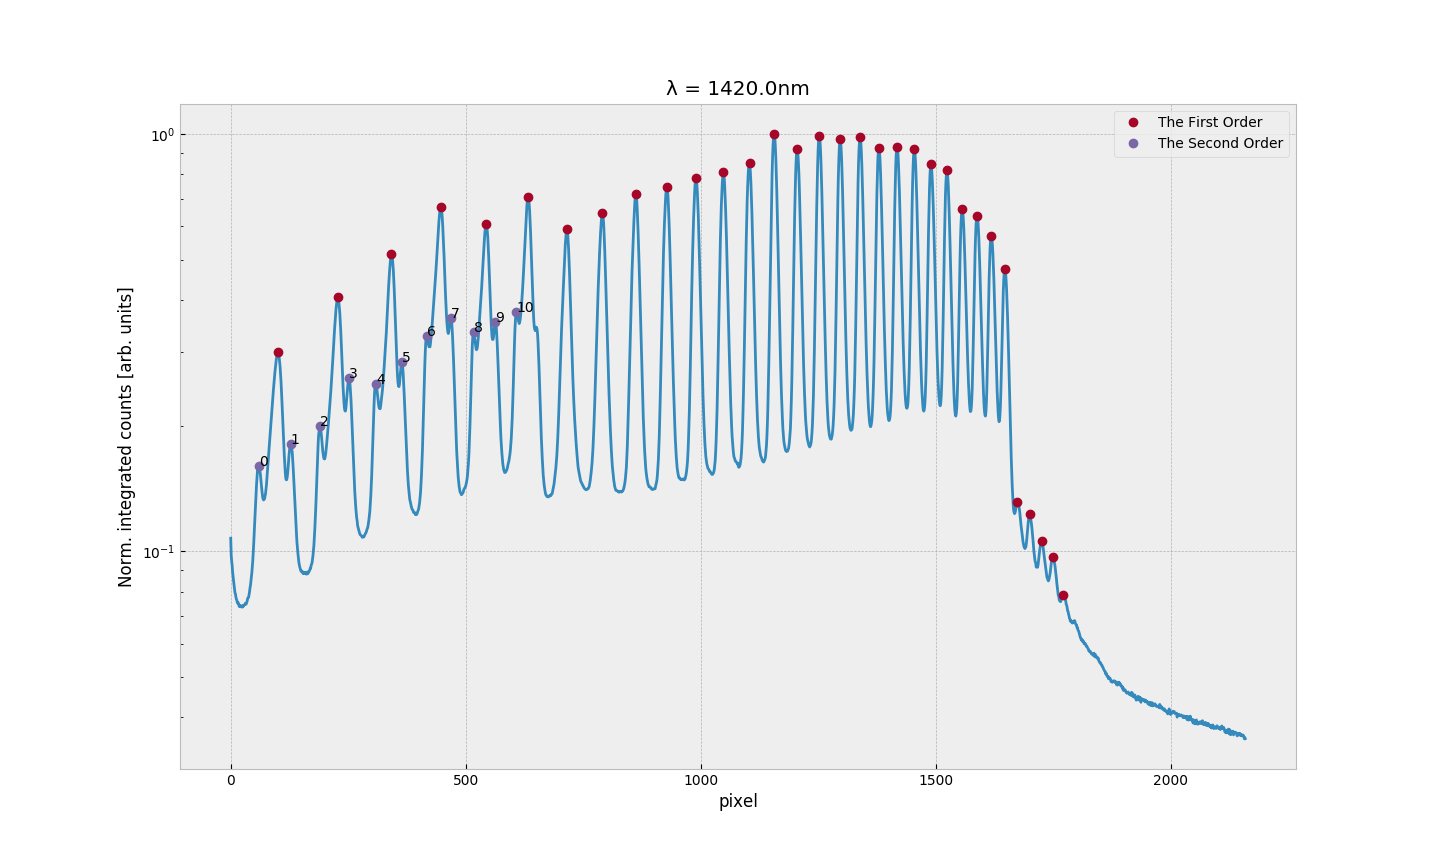
\includegraphics[width=0.9\textwidth]{figures/Beamline/first_second_order_spectrum.png}
%	\caption{INCOMPLETE: multiple diffraction orders}
%	\label{fig:first_second_order}
%\end{figure}

%\begin{figure}
%	\centering
%	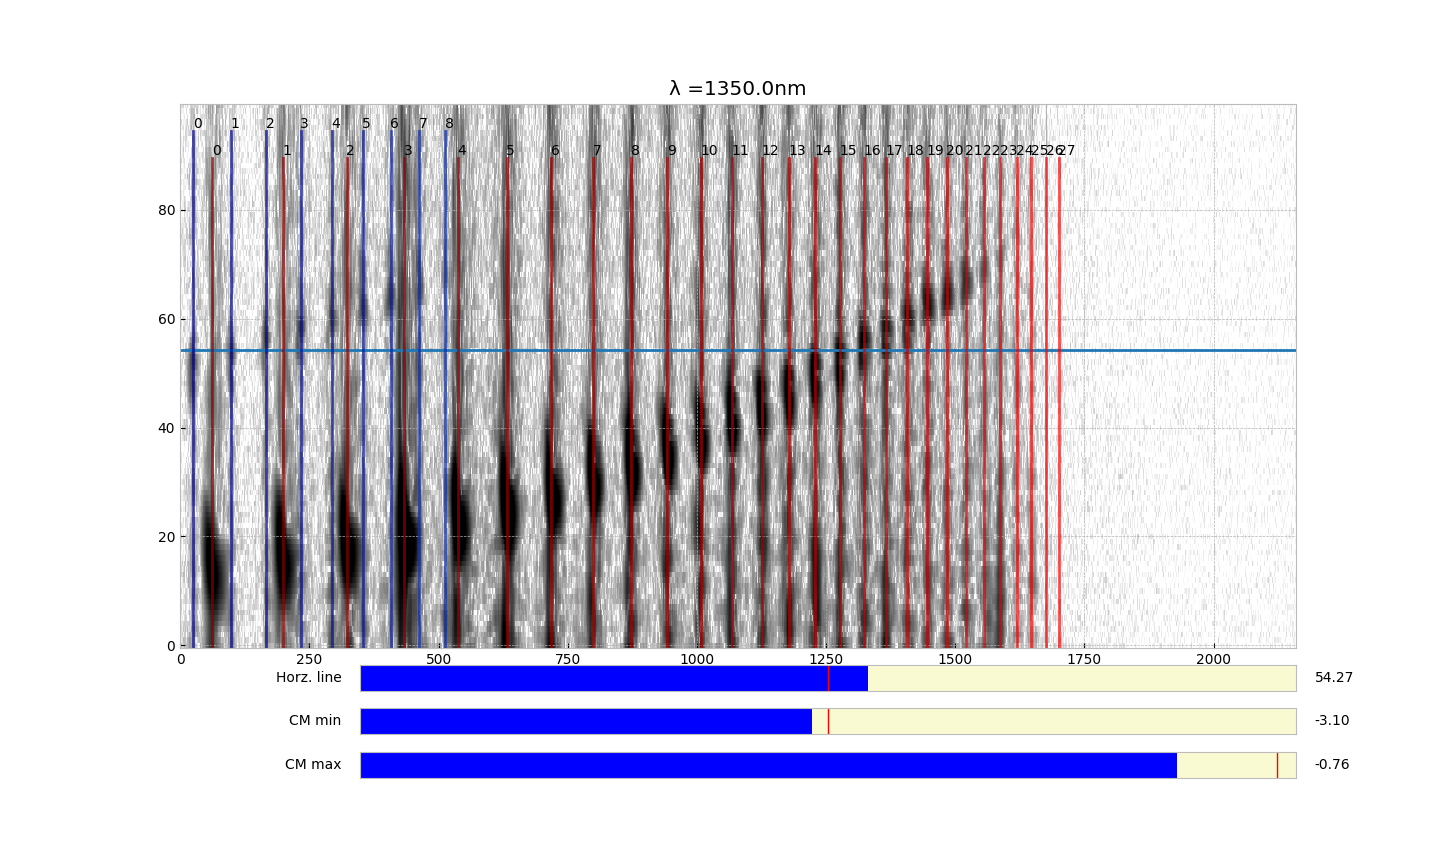
\includegraphics[width=0.9\textwidth]{figures/Beamline/line_matching_first_and_second.png}
%	\caption{INCOMPLETE: line matching}
%	\label{fig:line_matching}
%\end{figure}

%\begin{figure}
%	\centering
%	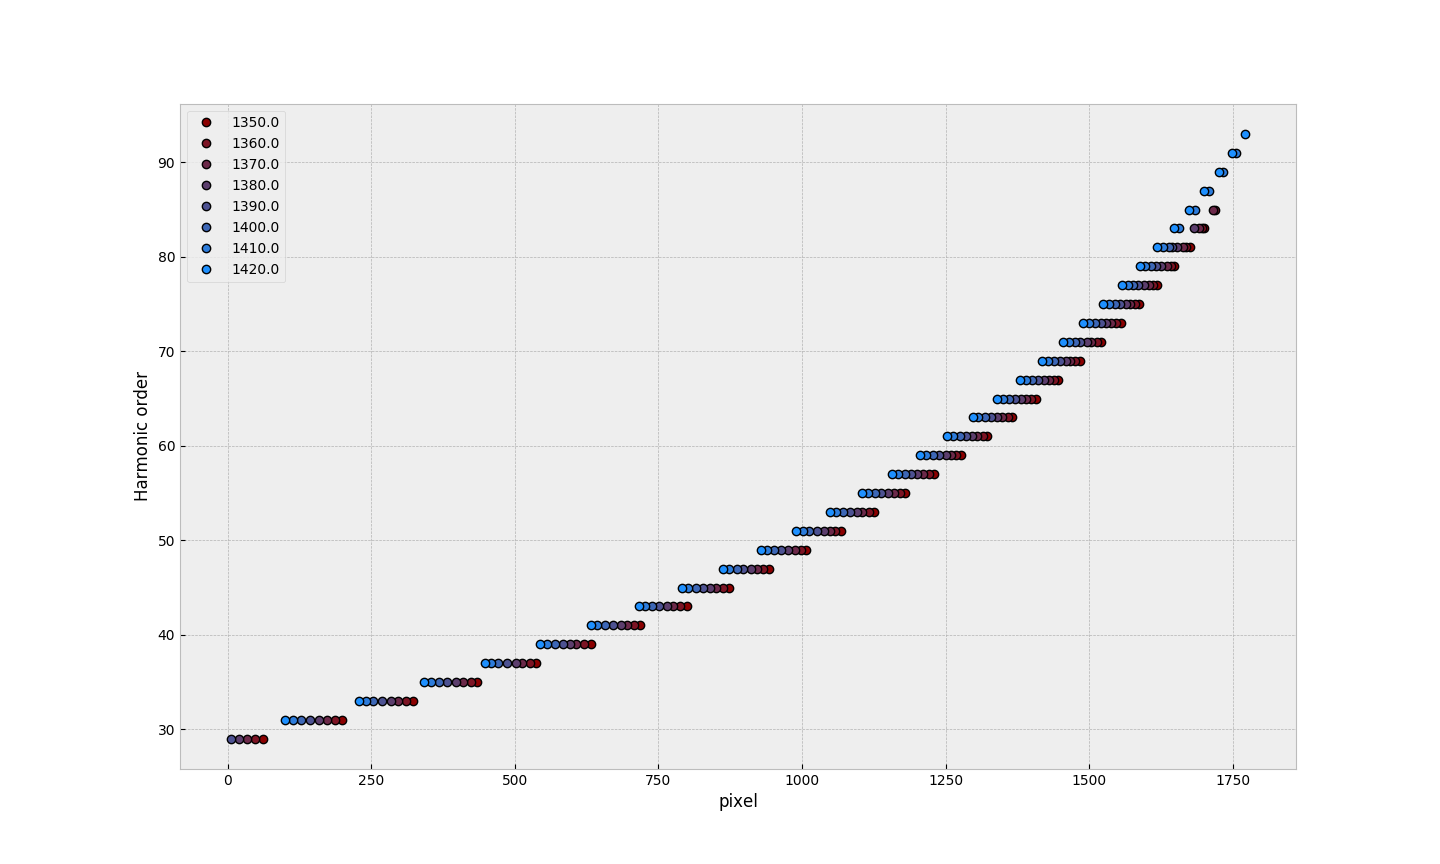
\includegraphics[width=0.9\textwidth]{figures/Beamline/harmonic order vs pixel.png}
%	\caption{INCOMPLETE: harmonic order vs pixel}
%	\label{fig:harm_order_vs_pixel}
%\end{figure}

%\begin{figure}
%	\centering
%	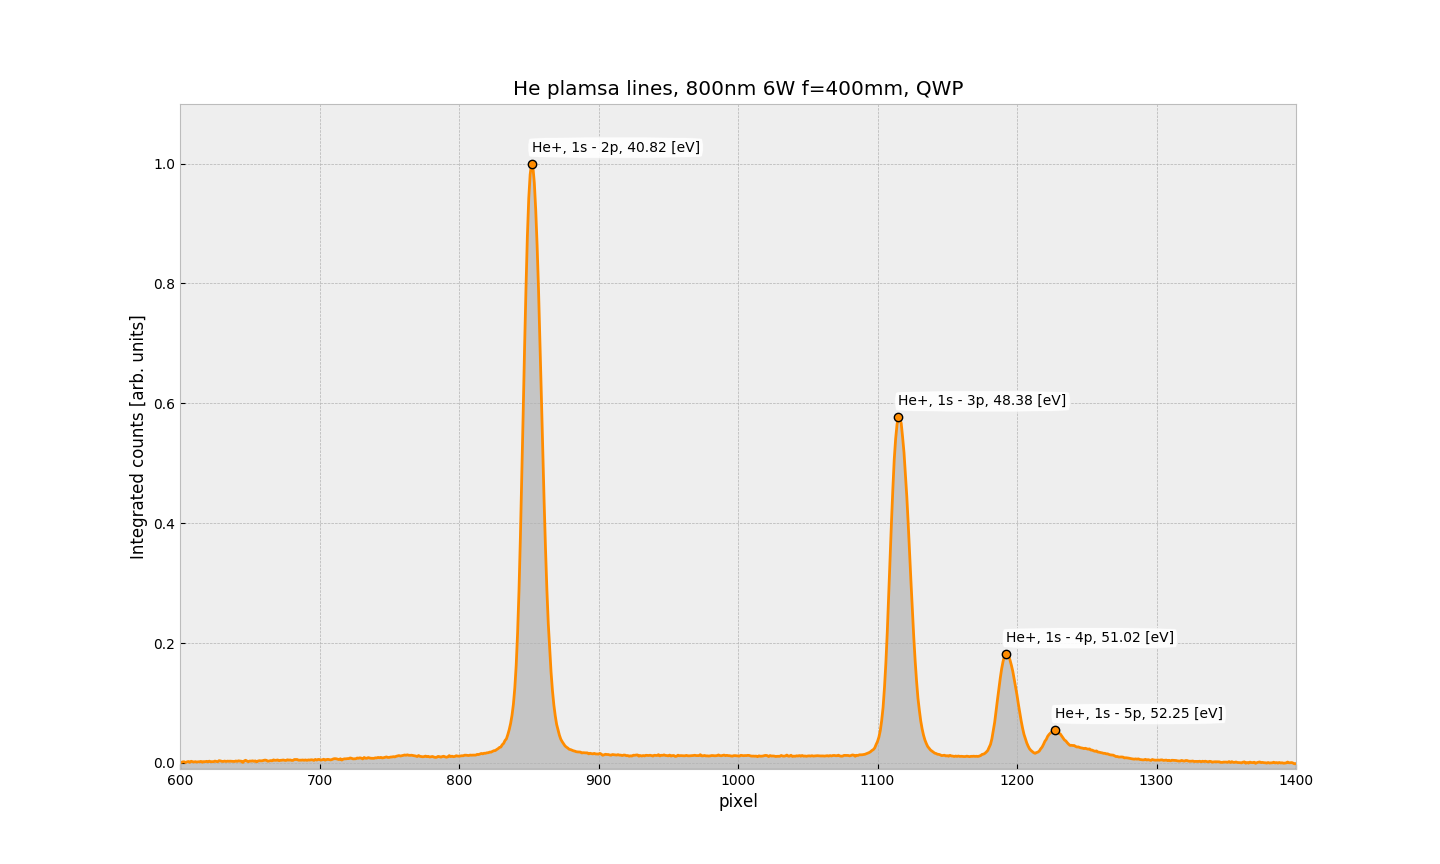
\includegraphics[width=0.9\textwidth]{figures/Beamline/He_plasma_line_spectrum.png}
%	\caption{INCOMPLETE: he plasma lines}
%	\label{fig:He_plasma_lines}
%\end{figure}

%\begin{figure}
%	\centering
%	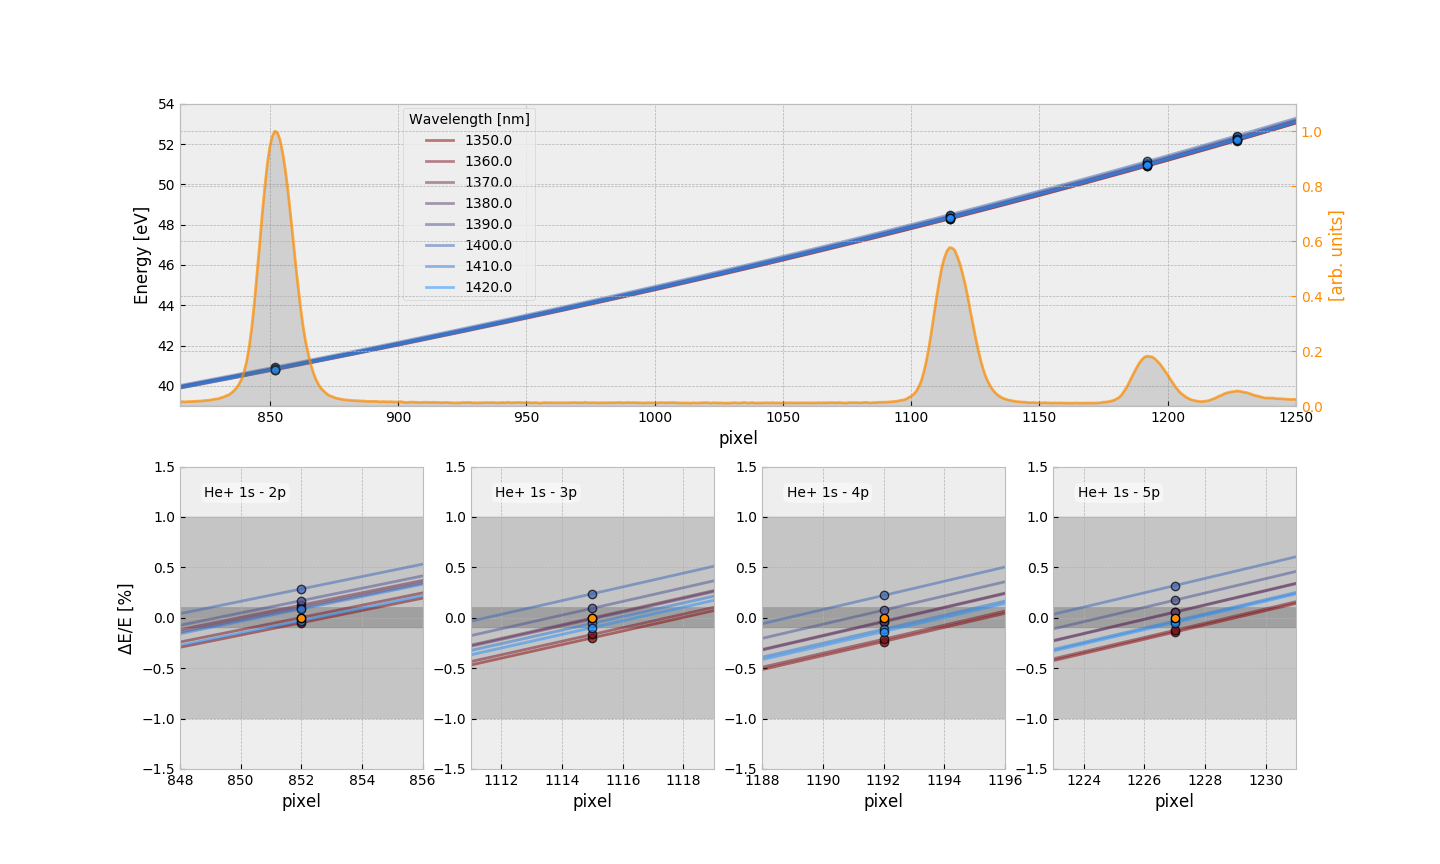
\includegraphics[width=0.9\textwidth]{figures/Beamline/He_plamsa_line_comparison.png}
%	\caption{INCOMPLETE: he plasma lines comparison}
%	\label{fig:plamsa_line_comparison}
%\end{figure}




\include{chapter_swpg}
\chapter{Two-source Fourier Transform Spectroscopy}
\label{chap:refractive_index}

\section{Introduction}
\label{intro_ts}
In chapter \ref{chap:two_source}, the $0-\pi$ square-wave phase grating (SWPG) was introduced as a means of generating two intense duplicates of an input femtosecond mid-IR pulse.  An additional element of the SWPG is that it enables precise control over the relative phase between these two sources.  When used to generate high harmonics, this scheme enables the generation of two XUV sources whose relative phase is well controlled by the SWPG, and any small phase shift between the two harmonic beams is imprinted upon their interference pattern as a fringe shift in the far-field.  The idea is to now leverage this sensitivity to measure an induced phase shift between the two XUV sources.  In the experiment described in this chapter, the phase shift will be induced by introducing a thin condensed matter sample into only one of the two XUV sources.  Doing so enables us to extract both the real and imaginary part of the refractive index over a broad range of photon energies in the XUV.
\section{Complex refractive index}
The complex refractive index depends strongly on photon energy, and a cartoon of this is shown in figure \ref{fig:refractive_index_schematic}. We are interested in the refractive index in the XUV energy region, and in this energy region there are many resonances that correspond to transitions of core-level electrons to unoccupied states near the Fermi level (for the case of a condensed matter system)\cite{stohrNEXAFSSpectroscopy1992, attwoodSoftXraysExtreme2000}.  Complicated fine structure can emerge near these resonances that correspond to the local electronic and geometric environment\cite{stohrNEXAFSSpectroscopy1992, attwoodSoftXraysExtreme2000}.  Thus, the ability to measure both the real and imaginary parts of the complex refractive index can be important for many experiments using XUV light generated by HHG\cite{kaplanFemtosecondTrackingCarrier2018,  cirriAchievingSurfaceSensitivity2017}.

\begin{figure}
	\centering
	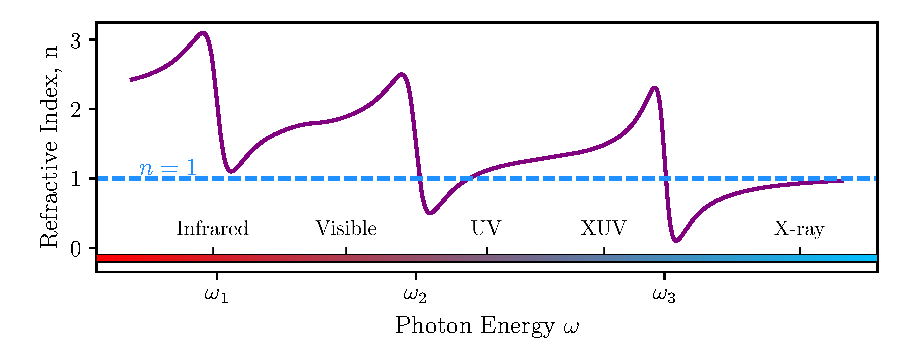
\includegraphics[width=1.0\textwidth]{figures/refractive_index/example_refractive_index.pdf}
	\caption[Schematic of real part of the refractive index from infrared to X-ray wavelengths]{Schematic of the real part of the refractive index versus photon energy. Example resonances are shown in the IR, the visible/UV, and in the XUV/soft x-ray regimes. In general, the refractive index approaches 1 at higher photon energies.}
	\label{fig:refractive_index_schematic}
\end{figure}

In general, the complex refractive index can be written as\cite{attwoodSoftXraysExtreme2000}
\begin{equation}
\label{eqn:refractive_index}
	n(\omega)=1 - \bigg(\frac{n_a r_e \lambda^2}{2\pi}\bigg)\bigg[f_1(\omega) - i f_2(\omega)\bigg]
\end{equation}
where $n_a$ is the number density, $\omega$ ($\lambda$) is the photon energy (wavelength), and
\begin{equation}
\label{eqn:r_e}
	r_e = \frac{e^2}{4\pi\epsilon_0 mc^2}
\end{equation}
is the classical electron radius. By introducing the parameters $\beta$ and $\delta$, such that
\begin{equation}
\label{eqn:delta_beta_def}
	\begin{aligned}
	\delta &= \frac{n_a r_e \lambda^2}{2\pi}f_1(\omega)\\
	\beta & = \frac{n_a r_e \lambda^2}{2\pi}f_2(\omega),
	\end{aligned}
\end{equation}
then the refractive index $n$ can be written as
\begin{equation}
\label{eqn:refractive_index_db}
	n(\omega)=1-\delta+i\beta.
\end{equation}
The values of both $\delta$ and $\beta$ have been tabulated for elements up to uranium in the range of 10 eV to 30 keV\cite{henkeLowenergyXrayInteraction1982}, and their values are generally smaller than unity when far from resonance.

Now that we've established the form of the refractive index, we will consider the case of propagation through a dispersive medium and its effect on amplitude and phase of a wave \cite{attwoodSoftXraysExtreme2000}. The idea is to consider a plane wave of the form
\begin{equation}
	\mathbf{E}(\mathbf{r},t)=\mathbf{E}_0e^{-i(\omega t - \mathbf{k}\cdot\mathbf{r})},
\end{equation}
and assume that the dispersion of the medium takes the form
\begin{equation}
	\frac{\omega}{k}=\frac{c}{1-\delta+i\beta}.
\end{equation}
With these relationships, one can write the field in the propagation direction defined by $\mathbf{k}\cdot\mathbf{r}=kr$ as
\begin{equation}
\label{eqn:wave_prop}
	\mathbf{E}(\mathbf{r},t)=\big(e^{-i\omega(t - r/c)}\big) \big(e^{-i(2\pi\delta/\lambda)r}\big) \big(e^{-(2\pi\beta/\lambda)r}\big).
\end{equation}
The first term in parentheses is the wave propagation, the second term is a phase shift proportional to $\delta$ that is induced by the dispersive medium, and the third term is a decay in amplitude that is proportional to $\beta$.  From this relationship, it can be shown that the attenuation of the intensity is given by 
\begin{equation}
\label{eqn:beer-lambert}
	\frac{I}{I_0}=e^{-(4\pi\beta/\lambda)r}=e^{-n_a \sigma_a r}
\end{equation}
where $I_0$ is the initial intensity and $\sigma_a=2r_\lambda f_2(\omega)$ is the photoabsorption cross section.  This relationship shows that by measuring the absorption of a material (a thin, free-standing film for these photon energies), one can easily extract the imaginary part of the refractive index.

The effect of the real part of the refractive index is to induce a phase shift in the propagating field, as can be seen from equation \ref{eqn:wave_prop}.  After propagating through a material of thickness $L$, the induced phase shift is given by
\begin{equation}
\label{eqn:phase_shift}
	\Delta\phi=\frac{2\pi\delta L}{\lambda}.
\end{equation}
To experimentally access this phase shift, a technique that can be used is interferometry \cite{hemmersDirectMeasurementComplex2012, hemmersMulticolorXUVInterferometry2009, wilsonDoubleSlitInterferometry2012}. The idea is to create a Mach-Zehnder interferometer (see figure \ref{fig:mach-zehnder_interferometer}), and in one of the arms introduce a sample of thickness $L$. By measuring how the interference patterns shift when introducing the sample, then one can directly measure the phase shift induced by the sample.  Additionally, by looking at how the fringe contrast changes, one can also get access to the attenuation caused by the sample.  This means that both the real and imaginary parts of the refractive index can be probed simultaneously.  This concept is precisely what will be used to extract the real and imaginary parts using the two XUV sources generated by a SWPG.  In that case each source will act as one arm of a Mach-Zehnder interferometer.
\begin{figure}
	\centering
	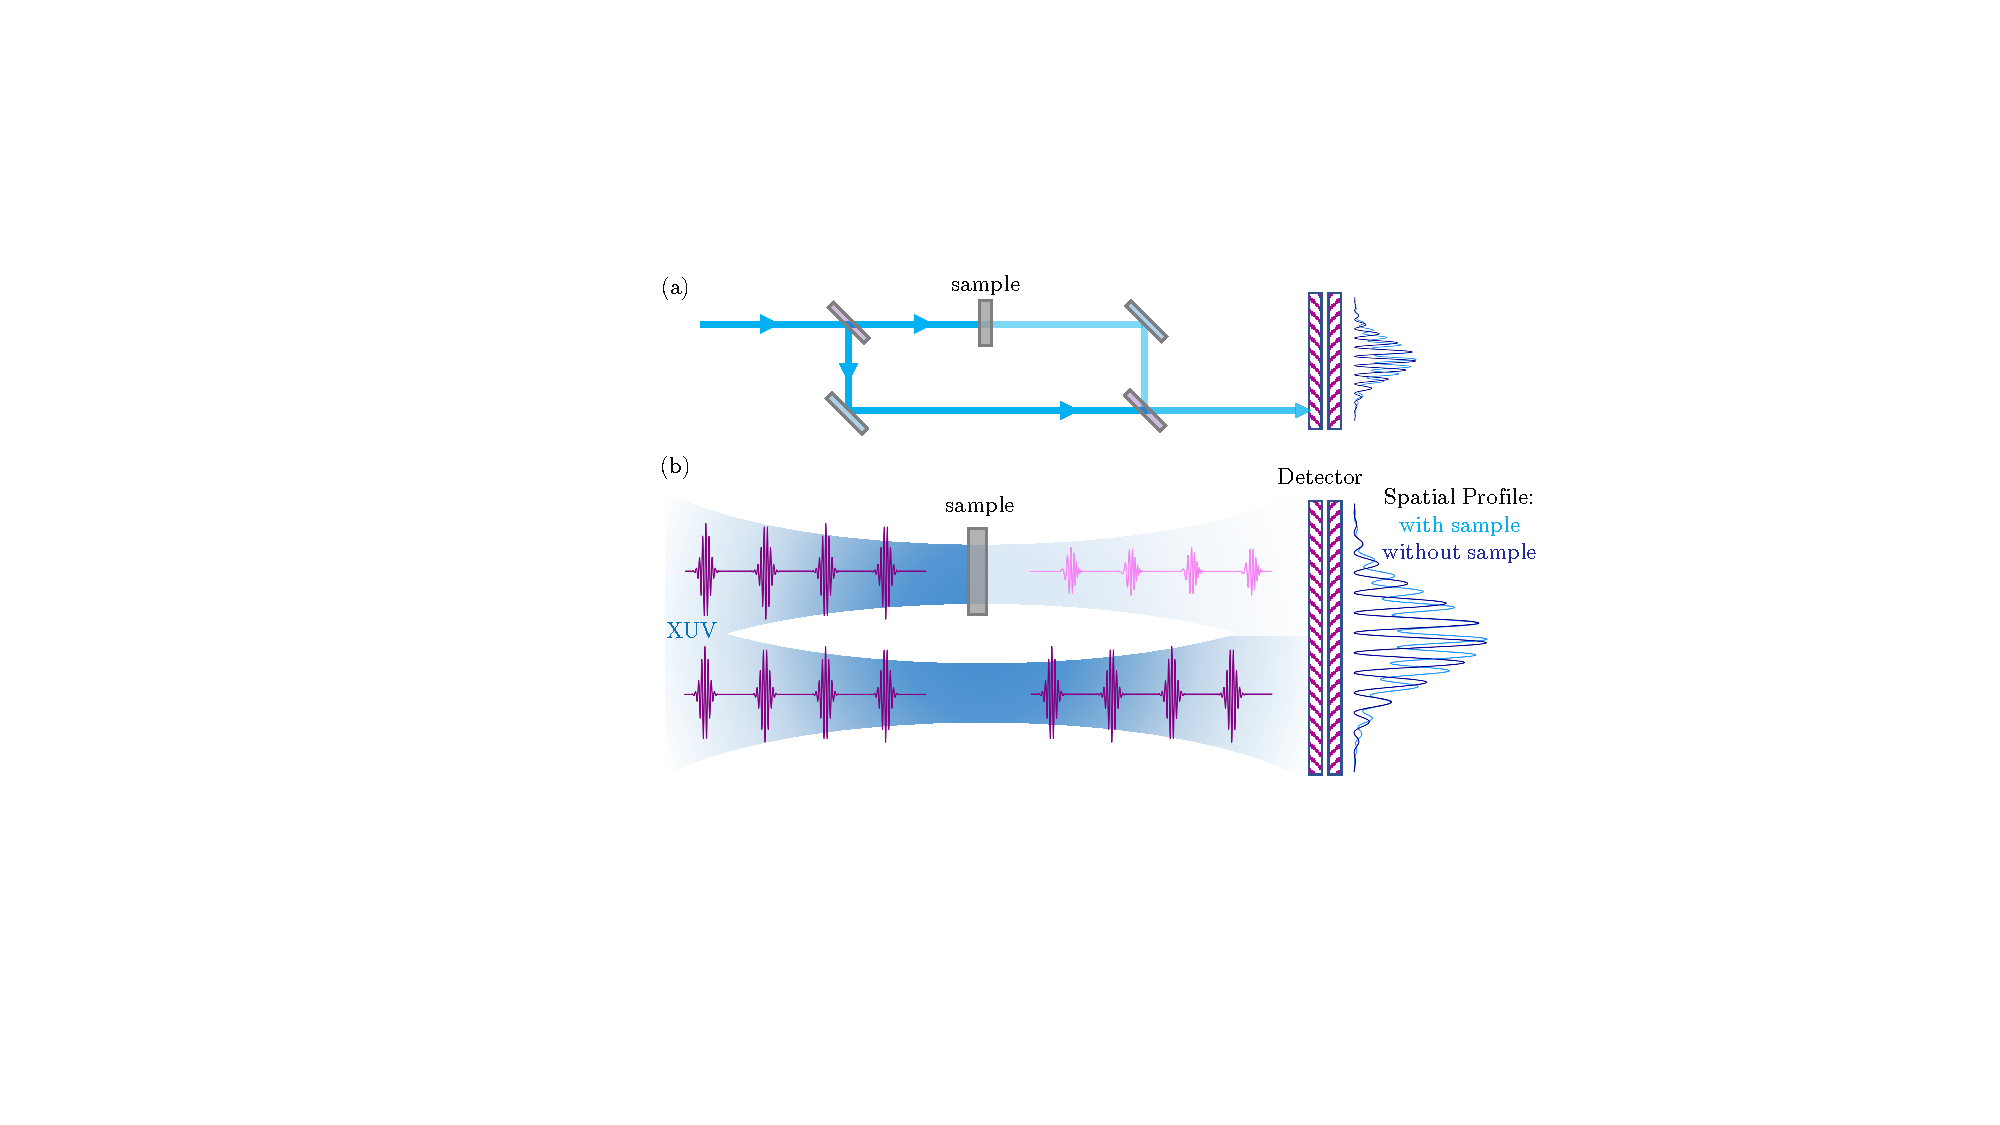
\includegraphics[width=0.8\textwidth]{figures/refractive_index/mach-zehnder_two_source.pdf}
	\caption[Schematic of Mach-Zehnder interferometer and spatial profile with and without a sample in one arm of the interferometer]{(a) Schematic of a Mach-Zehnder interferometer that is used to measure the phase shift induced by a sample placed in one of the arms of the interferometer. (b) For the experiments described in this chapter, the two XUV sources will act as the two arms of a Mach-Zehnder, and the sample of interest will only be introduced into one one the sources.}
	\label{fig:mach-zehnder_interferometer}
\end{figure}

\section{Measurement of the complex refractive index}
\subsection{Experimental setup}
\label{sec:experimental_setup_refrac}
The experimental setup that will be used to demonstrate the ability to measure both the real and imaginary parts of the refractive index is very similar to the experimental setup presented in chapter \ref{chap:two_source}.  The TABLe is the experimental beamline that will be used, and the setup is shown in figure \ref{fig:refract_schematic}.
\begin{figure}
	\centering
	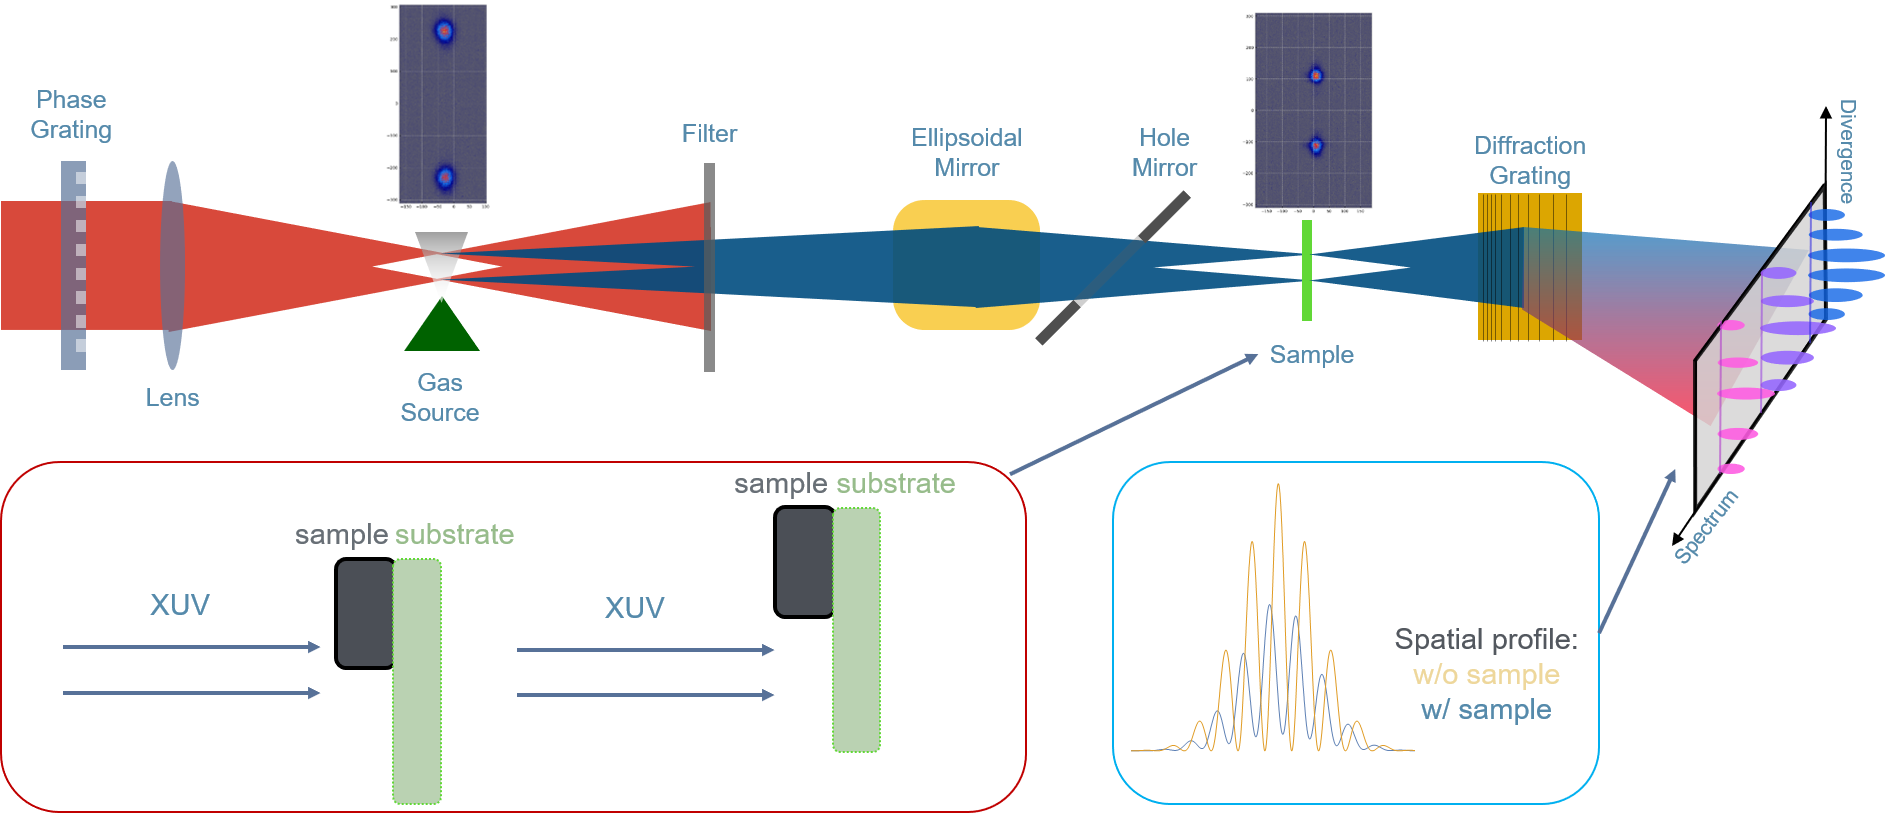
\includegraphics[width=0.8\textwidth]{figures/refractive_index/experimental_setup.png}
	\caption[Schematic of using two-source HHG to measure the real and imaginary part of the refractive index]{Schematic of the two-source HHG experiment performed in the TABLe. A $0-\pi$ SWPG is used to generate two intense lobes at the focus of a lens.  These lobes will generate XUV beams which will interfere in the far-field.  An ellipsoidal mirror is used to refocus the XUV beams into a target chamber before going onto the spectrometer. A sample that is shaped like a step-function will be introduced at the focus of the XUV in the target chamber.  The spatial profile of the various harmonic orders will be measured in the two cases shown.  The fringe shift and fringe contrast changes allow for a simultaneous measurement of both parts of the refractive index of the sample.}
	\label{fig:refract_schematic}
\end{figure}


\begin{figure}
	\centering
	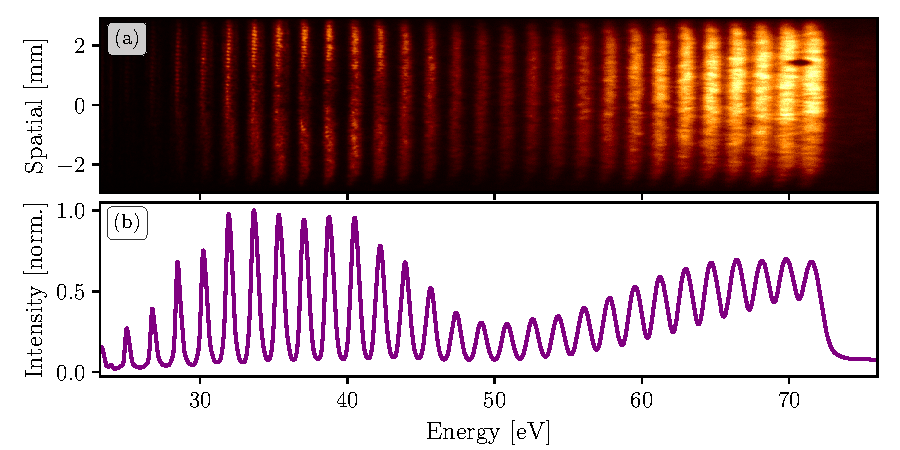
\includegraphics[width=1.0\textwidth]{figures/refractive_index/reference_img_spectrum.pdf}
	\caption[Reference image and spectrum of harmonics used to measure refractive index using SWPG]{Reference image (a) and harmonic spectrum (b) that was used in this experiment.  Fundamental wavelength is 1435 nm, and the harmonics are generated using an SWPG with a period of $d=2.5$ mm.}
	\label{fig:ref_img_spec}
\end{figure}
We use the output of the TOPAS at 1435 nm with a pulse energy of about 2 mJ and a pulse duration of around 70 fs. A $0-\pi$ SWPG is with a grating period of 2.5 mm is used to generate two intense lobes at the focal plane of a 400 mm focal length CaF2 plano-convex lens. At the focal plane, a gas medium is generated by a piezoelectric pulsed gas jet in which harmonics will be generated by the two sources.  The generation gas that will be used is argon. The fundamental wavelength is then filtered out by an aluminum filter.  The Al filter acts a high frequency band-pass with a band-pass region of 20-72 eV for the harmonic energies that are generated at this wavelength.  The harmonics are then refocused into a target chamber by an ellipsoidal mirror with a demagnification of three.  This entails that the source separation in the target chamber will be smaller by a factor of three, and the beam waist of each source will also be reduced by a factor of three.  This is where a sample will be introduced into only one of the two XUV sources. The sample in mounted on a motorized stage that allows for control of the position of the sample with respect to the XUV focus. After transmitting through the sample, the XUV will propagate to the spectrometer which allows for the spatial profile of each harmonic order to be measured.

In order to implement the scheme shown in figure \ref{fig:refract_schematic}, we need to introduce a sample into only one of the two XUV sources that are generated.  As mentioned previously, the source separation in the target chamber will be a third of the separation in the generation chamber. For the SWPG and laser parameters that we used for this experiment, the source separation in the harmonic generation chamber is $\Delta x=2\lambda f/d\approx460\:\mu m$, and the corresponding separation will be $\Delta x_t = \Delta x/3\approx153\: \mu m$ in the target chamber.  Therefore, the ideal sample has a cross sectional profile that is as close to a step function as possible, and the width of the step should be much less the separation between the two sources.  In general, this can be accomplished using photolithography techniques to pattern a thin film of the desired profile on top of a free standing membrane substrate.  For one of the samples that is used in this proof of principle experiment, we instead chose to start with a commercially available free standing membrane, and then break the membrane in such a way that it would have a sharp step-like cross sectional profile.  The membrane that was chosen was a free standing 260 nm single crystal Si membrane on a 500 $\mu$m Si frame.  These free standing membranes are manufactured by Norcada.  The sample needs to be this thin because this experiment is done in transmission and XUV is strongly absorbed by most materials. A schematic of the sample that was used is shown in figure \ref{fig:split_sample} (a).  A second sample was also fabricated using e-beam deposition of Ge on top of a 30 nm SiN free-standing membrane.  For this sample, shown in figure \ref{fig:split_sample} (b), a physical mask was used to cover half of the SiN membrane before deposition.  Due to the delicate nature of these free-standing membranes, the physical mask could not touch the membrane without breaking it, and this necessitated a small gap between the physical mask and the membrane itself.  The result of this gap is that there will be a more gradual change in thickness between the two halves of the sample (with and without Ge).

\begin{figure}
	\centering
	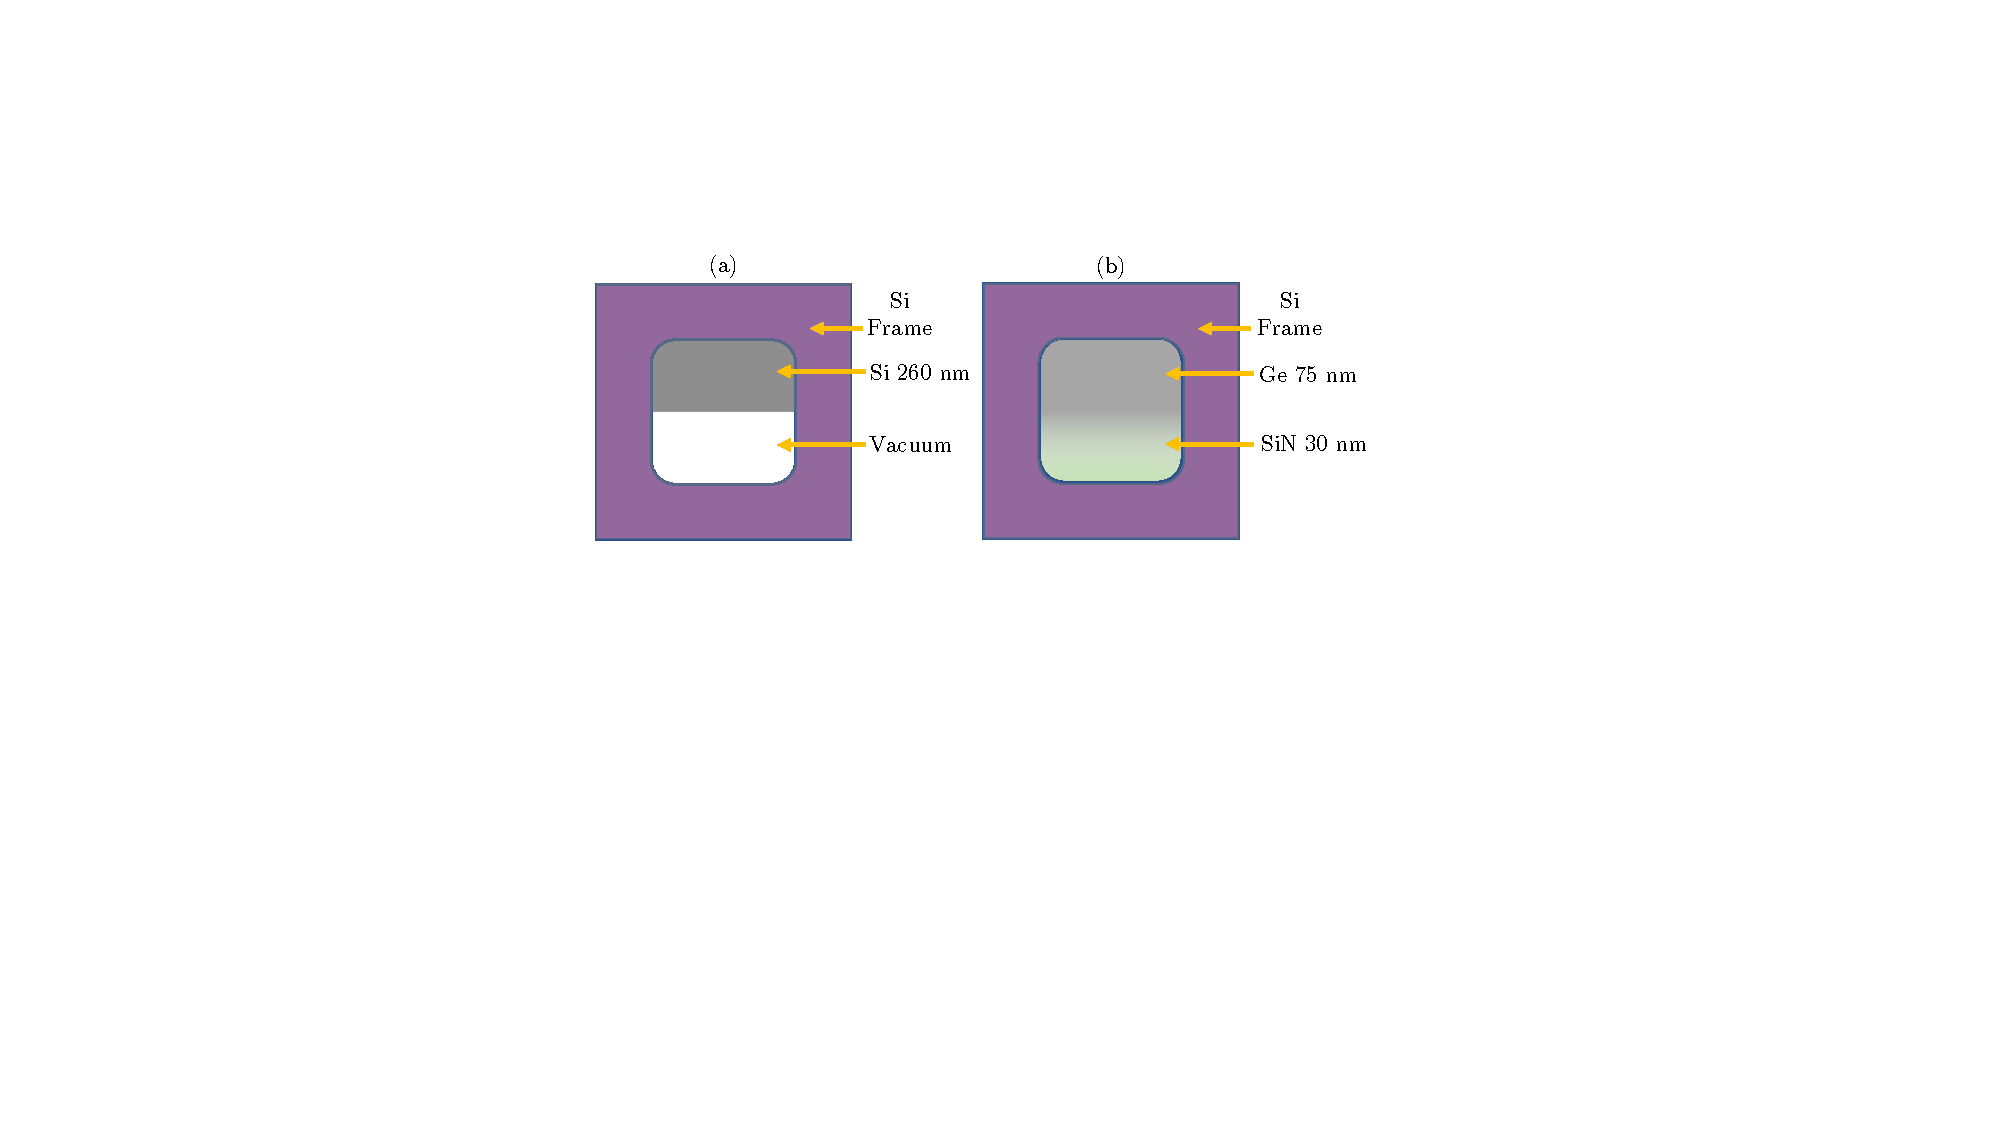
\includegraphics[width=0.8\textwidth]{figures/refractive_index/samples.pdf}
	\caption[Schematic of the samples used to measure the refractive index of silicon and germanium]{Schematic of the samples that were used in this experiment.  (a) Free standing 260 nm Si membrane that has been broken in half.  The way that the sample was cleaved in half ensures that the edge is sharper than the separation between the two sources.  The sample was made by Norcada before it was broken. (b) Germanium deposited on a free standing 30 nm SiN membrane.  E-beam deposition was performed with a physical mask to create a step-like profile.}
	\label{fig:split_sample}
\end{figure}


\begin{figure}
	\centering
	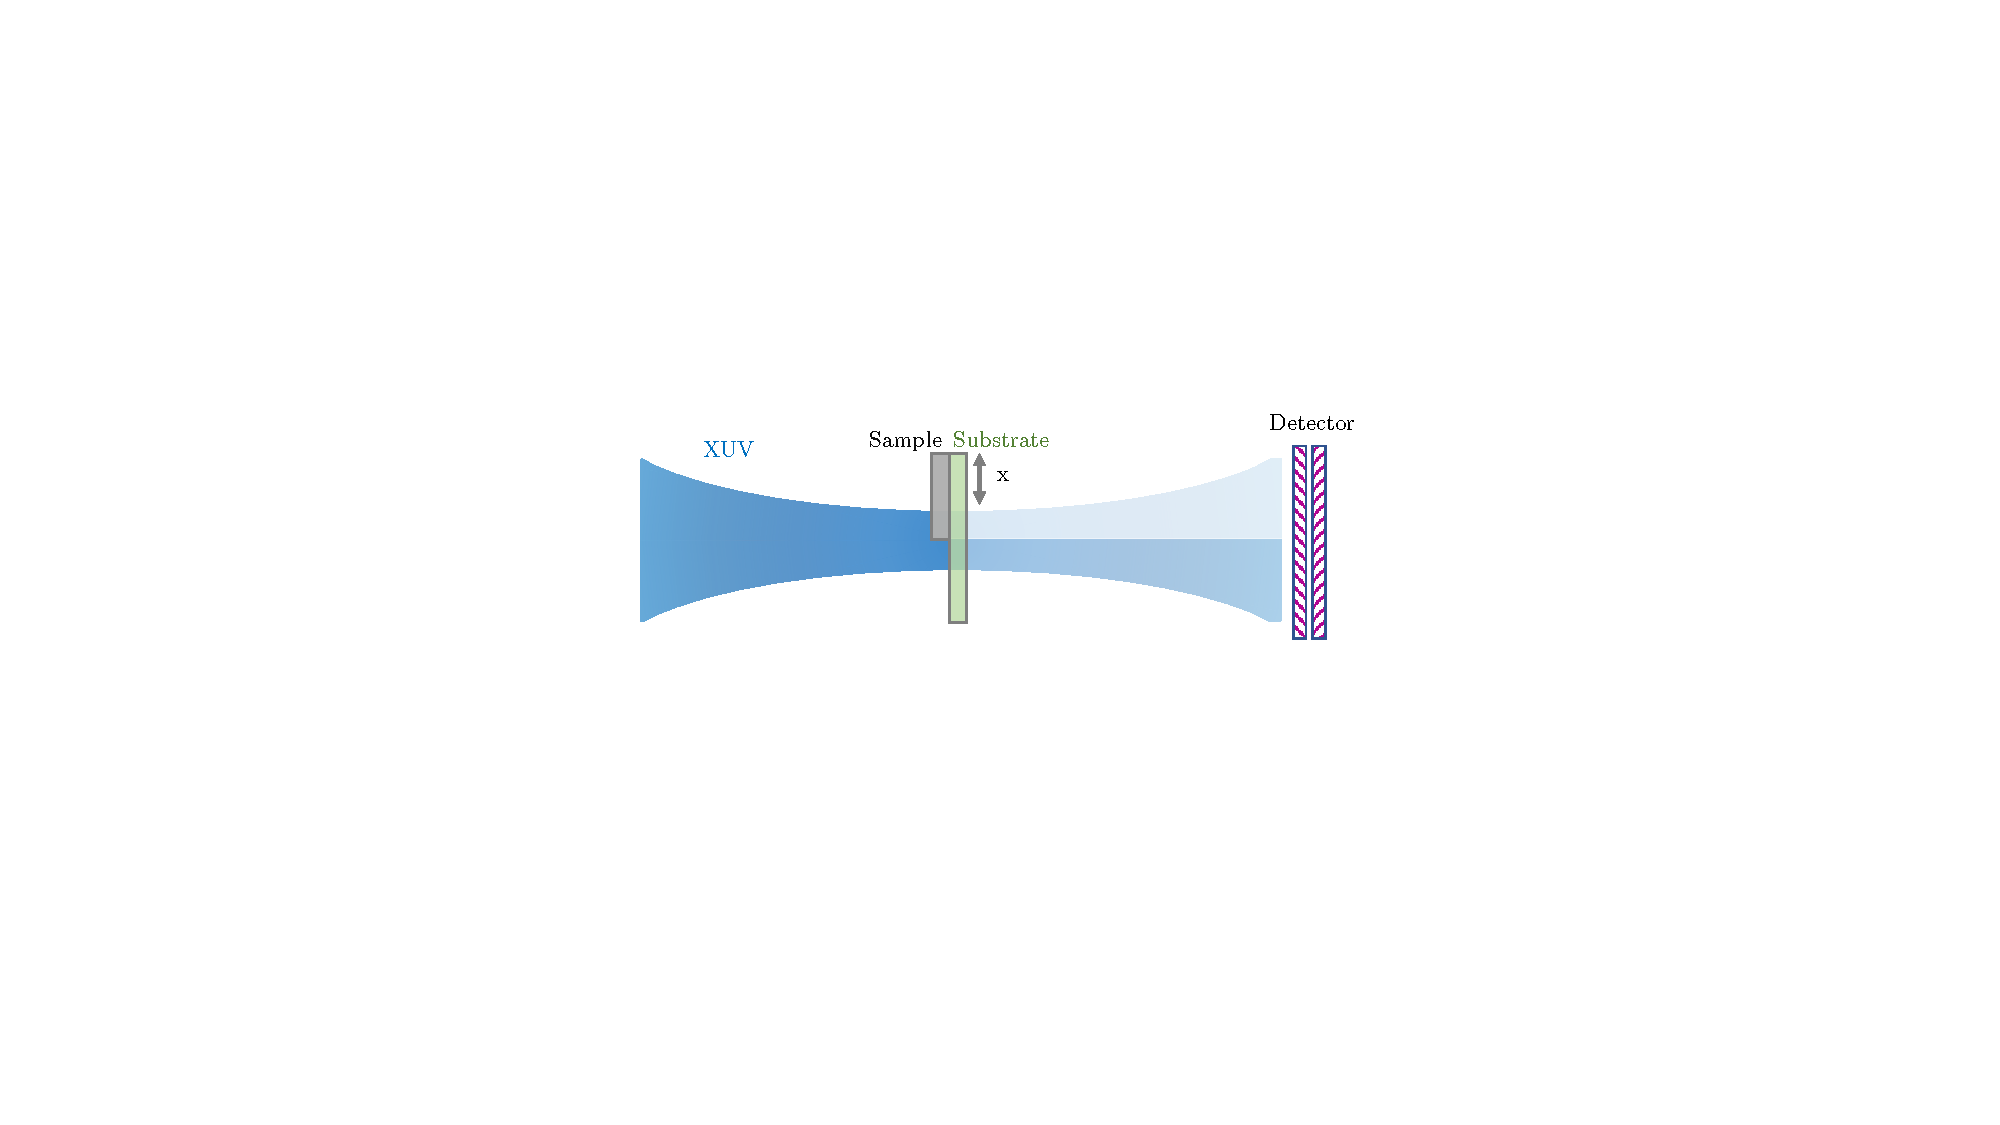
\includegraphics[width=0.7\textwidth]{figures/refractive_index/knife_edge.pdf}
	\caption[Schematic of knife edge technique used as a profilometry tool]{Schematic of knife edge technique used as a profilometry tool.  A transmissive sample and substrate are translated through the focus of the XUV, and the detected harmonic amplitude as a function of position can be used to reconstruct the beam and transmission profiles.}
	\label{fig:knife_edge_schematic}
\end{figure}

To be more precise about the cross sectional profile of the fabricated samples that were used, a form of profilometry was performed using the XUV beam as a probe of the thickness of the sample.  The idea is simply an extension of the knife edge method that is used to measure beam profiles, see section \ref{sec:xuv_beam_size_knife_edge} for the basics.  In this case, the assumption that the knife is totally opaque is lifted and the transmission function of the sample is included.  The total transmitted power in this case now becomes
\begin{equation}
	\label{eqn:transmission_knife_edge_power}
	P(x, \omega) = \int_{\infty}^{\infty}\int_{\infty}^{\infty} T(x - x', \omega) I(x', y')\diff x' \diff y
\end{equation}
where $T(x, E)$ is the transmission of the sample as a function of position and energy.\footnote{For the case of a opaque knife, $T = \Theta(x - x')$ and equation \ref{eqn:knife_edge_power} is recovered.} This essentially represents the spatial convolution of the transmission profile of the sample with the beam profile.  Generally, in order for this to be useful as a profilometry tool, the beam size must be much smaller the feature sizes of the transmission profile.  If this is not the case, then \emph{a priori} knowledge of either the beam profile or the transmission profile is needed to reconstruct the other profile.  As seen in section \ref{sec:xuv_beam_size_knife_edge}, the beam profile can be independently measured using part of the sample frame to determine the beam profile.  If the beam width can be treated as vanishingly small relative to the transmission profile, then the total transmitted power becomes
\begin{equation}
	\label{eqn:knife_edge_delta}
	P(x,\omega) = P_0(\omega)T(x,\omega).
\end{equation}
To determine the thickness profile of the sample some assumptions are need.  If one assumes knowledge of the absorption cross section as a function of energy, then Beer-Lambert's Law can be used directly to calculate the thickness, see equation \ref{eqn:beer-lambert}.  Additionally, if one assumes knowledge of the maximal thickness $d_0$ of the sample on top of the substrate, then the total transmitted power becomes
\begin{equation}
	\label{eqn:trans_power_thickness_assumed}
	P(x,\omega) = P_0(\omega)T(x,\omega) = P_0(\omega)T_0(\omega)^{d(x)/d_0}
\end{equation} 
where $T_0$ is the transmission at the maximal thickness $d_0$.  This allows for calculation of the thickness profile from the integrated harmonic signal, and the resulting relationship is 
\begin{equation}
	\label{eqn:thickness_calc}
	d(x) = d_0\bigg(\frac{\log \overline{C}(x)}{\log \overline{T_0}}\bigg)
\end{equation}
where $\overline{C}$ and $\overline{T_0}$ are the integrated average harmonic counts and maximal transmission.

This method is used to measure the profile of the samples that were used in this experiment.  The results of these measurements are shown in figure \ref{fig:knife_edge_samples}.  The integrated harmonic signal is shown in purple and shows a very sharp step for the Si sample whose width is limited by the harmonic beam waist of 6 $\mu$m, however the Ge sample shows a much broader transition region between the two regions that is approximately 200 $\mu$m in width.  This was to be expected from the type of physical mask used to make the Ge sample, and it could be improved upon by implementing photolithography techniques.  That being said, these samples are of sufficient quality to demonstrate the technique of measuring the complex refractive index using the SWPG.
\begin{figure}
	\centering
	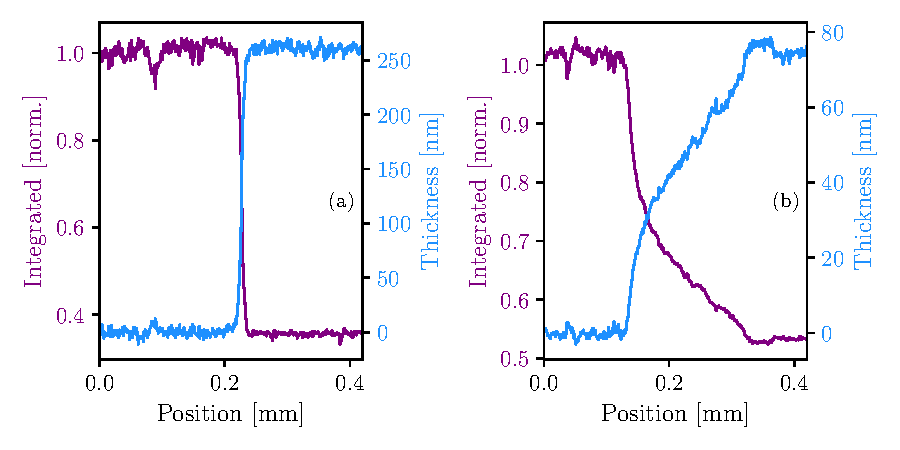
\includegraphics[width=1.0\textwidth]{figures/refractive_index/integrated_knife_edge.pdf}
	\caption[Profilometry using integrated XUV signal for both Si and Ge samples]{Integrated XUV signal (purple) as samples in shown in figure \ref{fig:split_sample} are translated in the focal plane.  Result is a profilometry measurement using XUV to characterize the thickness profile (blue) of the two samples with Si sample shown in (a) and the Ge sample in (b).}
	\label{fig:knife_edge_samples}
\end{figure}

\subsection{Results}
To measure the complex refractive index of the samples shown in figure \ref{fig:split_sample}, we will look for a fringe shift and change in fringe contrast when only one of the sources is going through the sample and the other is going through either vacuum or the substrate.  To see this, we translate the sample through the focal plane in the target chamber such that three distinct regimes will occur.  The first is when both sources are going through vacuum/substrate, the second is when one source is going the sample and the other is going through vacuum/substrate, and the final regime is when both sources are going through the sample.  Since this is a differential measurement, we would only expect to see a fringe shift for the second regime.  The first and third regimes should show the same fringe pattern, and the only expected difference is the overall modification of the spectral amplitude of the harmonics due the absorption of the sample.  This is shown in figure \ref{fig:harmonic_phase_shift} (b) for the Si sample and figure \ref{fig:harmonic_fringe_shift_contrast_ge} (b) for the Ge sample, where the spatial profile is shown for harmonic order 29 and 37 as the sample is translated through the focal plane.

From the spatial profile shown in figure \ref{fig:harmonic_phase_shift} (b), the three expected regimes can clearly be seen.  There is also additional spatial structure that is present in the transition between each of the three regimes.  This is due to diffraction that is caused by one of the sources being partially blocked.  From the spatial profile, the fringe shift can be extracted from the spatial frequency component that corresponds to this harmonic.  The phase of that spatial frequency is plotted in \ref{fig:harmonic_phase_shift} and shows that there is a phase shift between the two sources when only one of the sources is going the sample.  From this phase shift it is now possible to calculate the real part of the refractive index from the relationship
\begin{equation}
	\label{eqn:fringe_shift_x}
	\delta = \frac{\lambda\Delta\phi}{2\pi\Delta d}
\end{equation}  
where $\Delta d$ is the thickness difference and $\Delta \phi$ is the phase shift between the two sources.  The phase shift that is observed in harmonic order 29 can be seen across the harmonic spectrum, and enables the real part of the refractive index to be extracted across a broad range of photon energies simultaneously.  Similar behaviour is observed for the Ge sample in figure \ref{fig:harmonic_fringe_shift_contrast_ge} (b), however the broad thickness profile of the sample causes a gradual transition between the three regimes as each sources transmits through varying thickness of Ge.  That being said, the phase shift that is observed can still be used to measure the real part of the refractive index, just at an effective thickness given by the difference in thickness of Ge between each source.

\begin{figure}
	\centering
	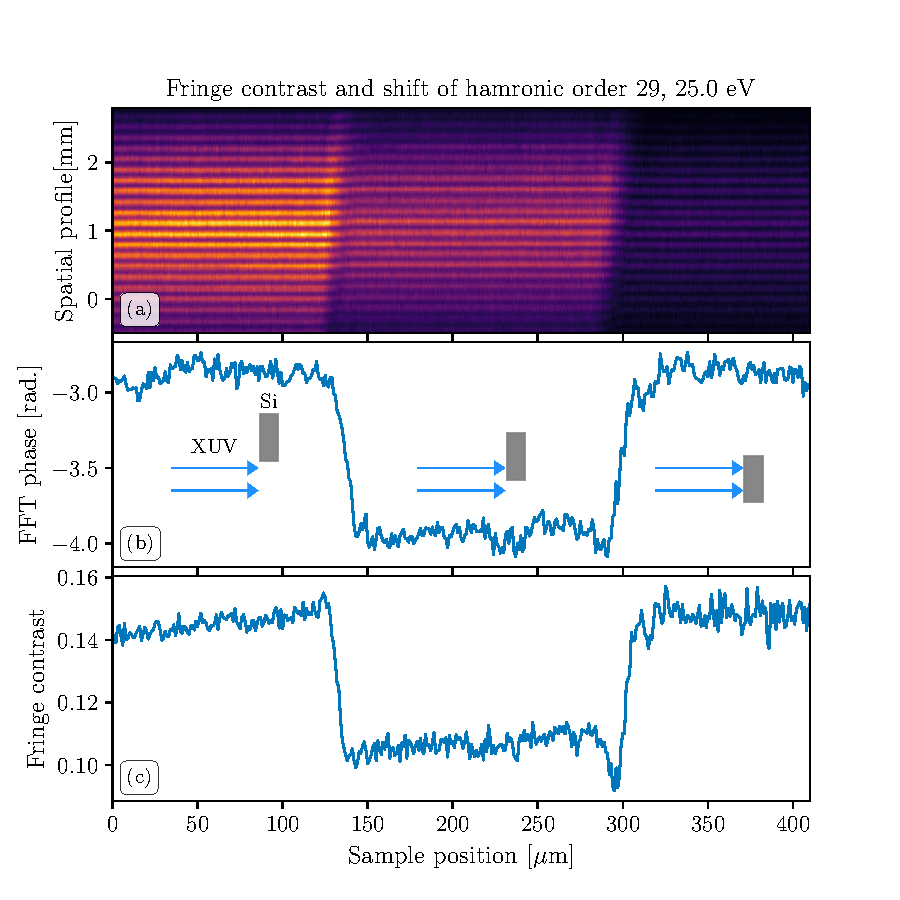
\includegraphics[width=1.0\textwidth]{figures/refractive_index/spatialgram_fringe_shift_contrast.pdf}
	\caption[Spatial profile and fringe shift of a harmonic as sample is translated across the two XUV sources]{(a) Spatial profile of harmonic order 29 as the silicon sample is translated through the two sources. Three regimes are clear from the spatial profile, and they correspond to both sources going through vacuum, only one source going through the sample, and both sources going through the sample.  A clear fringe shift can be seen between the second regime and the other two.  Additional structure is seen at the transition between regimes, and this is due to diffraction cause by the sample partially blocking one of the sources. (b) Phase extracted from the spatial frequency corresponding to this harmonic order.  The phase shift induced by the Si sample can be extracted from this phase shift. (c) Fringe contrast extracted from the spatial frequency corresponding to this harmonic order.}
	\label{fig:harmonic_phase_shift}
\end{figure}

\begin{figure}
	\centering
	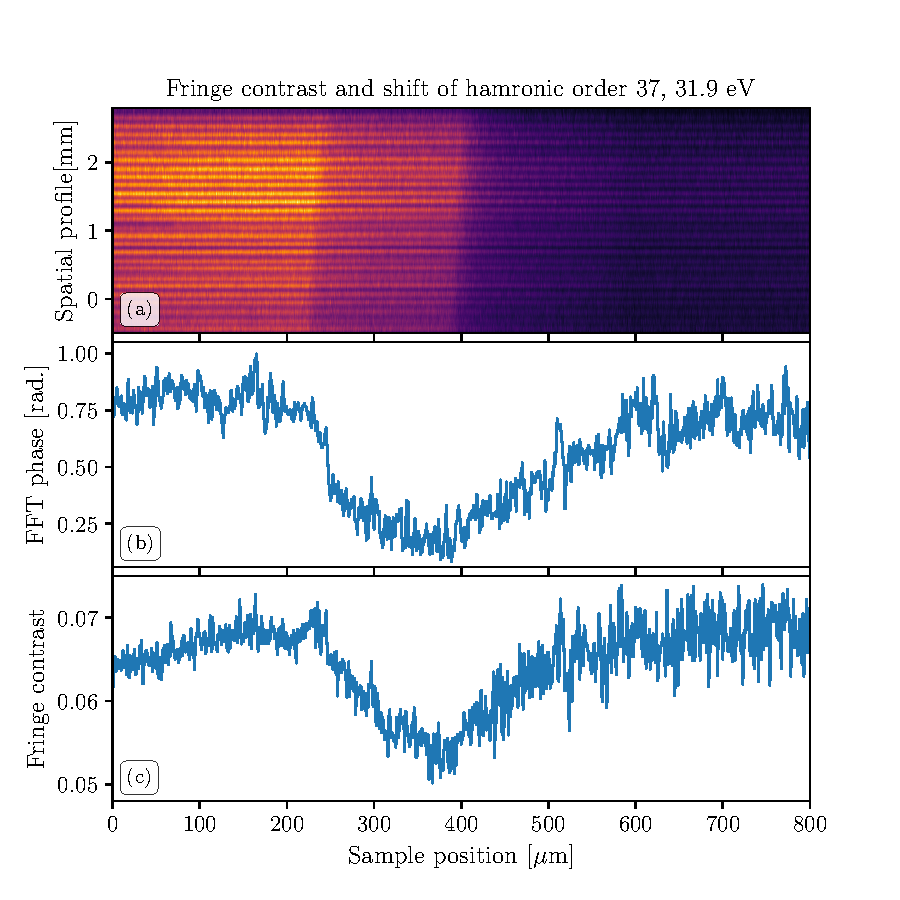
\includegraphics[width=1.0\textwidth]{figures/refractive_index/spatialgram_fringe_shift_contrast_ge.pdf}
	\caption[Spatial profile and fringe shift of a harmonic as sample is translated across the two XUV sources]{(a) Spatial profile of harmonic order 37 as the germanium sample is translated through the two sources. Three regimes are clear from the spatial profile, and they correspond to both sources going through vacuum, only one source going through the sample, and both sources going through the sample.  A clear fringe shift can be seen between the second regime and the other two.  Additional structure is seen at the transition between regimes, and this is due to diffraction cause by the sample partially blocking one of the sources. (b) Phase extracted from the spatial frequency corresponding to this harmonic order.  The phase shift induced by the Si sample can be extracted from this phase shift. (c) Fringe contrast extracted from the spatial frequency corresponding to this harmonic order.}
	\label{fig:harmonic_fringe_shift_contrast_ge}
\end{figure}


In addition to the fringe shift that is show in figure \ref{fig:harmonic_phase_shift} (b), there is also a change in fringe contrast that can be seen as the sample is translated through the two sources.  In general, the fringe contrast can be defined as the relative difference of of the maximum and minimum values of an interference pattern, such that
\begin{equation}
	V=\frac{I_{\mathrm{max}} - I_{\mathrm{min}}}{I_{\mathrm{max}} + I_{\mathrm{min}}} = \frac{I_{\mathrm{amp}}}{I_{\mathrm{mean}}}
\end{equation}
is the fringe visibility or contrast.  When considering the case of two interfering beams, this fringe contrast can be written as
\begin{equation}
\label{eqn:fringe_visibility} 
	V = \frac{2\sqrt{I_1 I_2}}{I_1 + I_2}\gamma_{12}
\end{equation}
where $I_1$ and $I_2$ are the intensity of the two beams and $\gamma_{12}$ is the coherence between them \cite{hemmersMulticolorXUVInterferometry2009, ditmireSpatialCoherenceMeasurement1996, wilsonDoubleSlitInterferometry2012}. 
This change in fringe contrast is shown in figures \ref{fig:harmonic_phase_shift} (c) and \ref{fig:harmonic_fringe_shift_contrast_ge} (c).  The contrast shows the same three distinct regimes that were seen in the fringe shift.  Similarly to the fringe shift, it can be seen that there is only a change in fringe contrast when only one of the sources is going through the sample.  From this contrast, it is possible to calculate the imaginary part of the refractive index.  This can be done using the relationship
\begin{equation}
\label{eqn:beta_fringe_contrast}
	\beta = -\frac{\lambda}{2\pi \Delta d} \ln\Bigg[\frac{V_0}{V}\Bigg(1-\sqrt{1-\bigg(\frac{V}{V_0}\bigg)^2}\Bigg)\Bigg]
\end{equation} 
where $V_0$ is the contrast without the sample and $V$ is the contrast with the sample present in one of the sources \cite{hemmersMulticolorXUVInterferometry2009}.



\begin{figure}
	\centering
	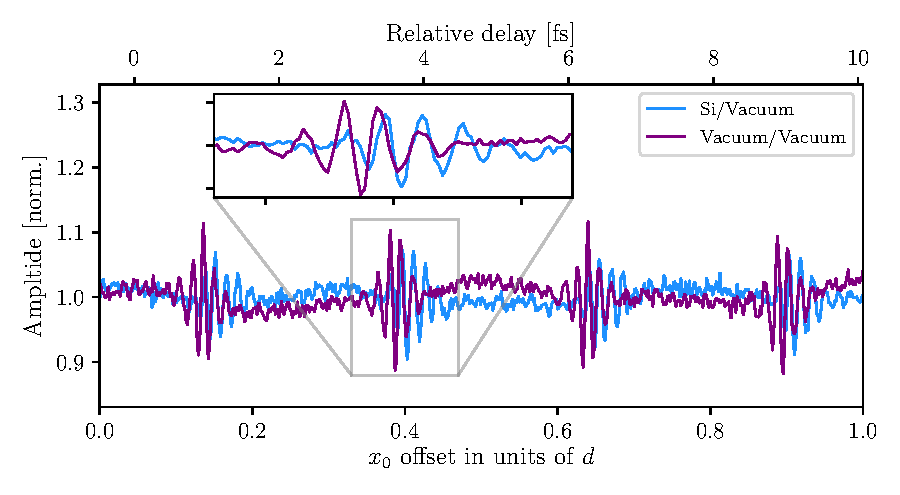
\includegraphics[width=1.0\textwidth]{figures/refractive_index/cross_correlation_si.pdf}
	\caption[Interferogram of all harmonic orders with and without Si sample in one source]{Interferogram of all harmonic orders that is extracted from the combined spatialgram with and without Si sample in one source.  The shift between the two cases is 162 as in relative delay.}
	\label{fig:interferogram_si}
\end{figure}

\begin{figure}
	\centering
	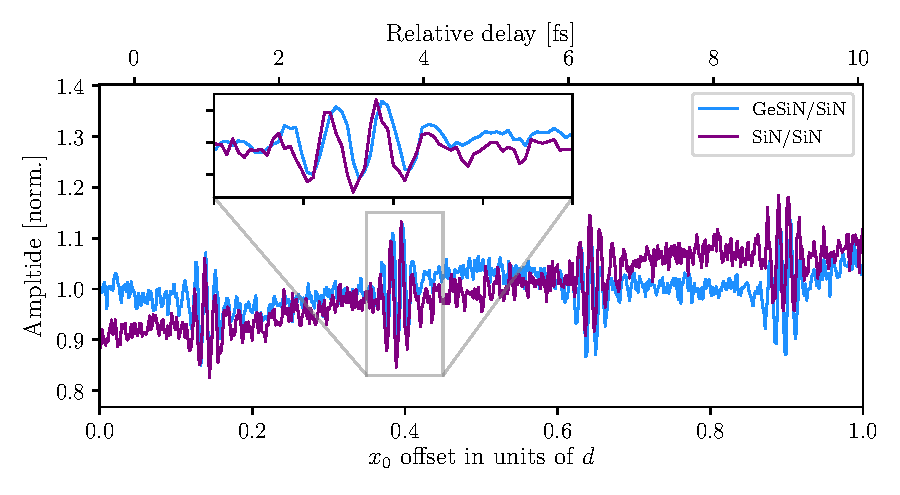
\includegraphics[width=1.0\textwidth]{figures/refractive_index/cross_correlation_ge.pdf}
	\caption[Spatialgram of combined harmonic orders with and without Ge sample in one source]{Spatialgram of combined harmonic orders with and without Ge sample in one source. The shift between the two cases is 16 as in relative delay.}
	\label{fig:interferogram_ge}
\end{figure}

An additional parameter that can be uniquely controlled by using the SWPG is the relative phase between the two XUV sources that are generated, as was established in chapter \ref{chap:two_source}. To leverage this capability, the position of the SWPG can be translated through the beam profile to linearly vary the relative phase between the two sources at two different positions along the thickness profile of the samples.  The obvious candidates for these positions along the thickness profile are: (1) only one source transmits through the sample and the other transmits through the substrate/vacuum and (2) both sources transmitting through the substrate/vacuum.  Intuitively, one would expect to see an additional phase shift between the two sources that is given by equation \ref{eqn:phase_shift}.  To see how this phase shift manifests itself, the interferogram of all harmonic orders that is extracted from the combined spatialgram is shown in figure \ref{fig:interferogram_si} and figure \ref{fig:interferogram_ge} for the two positions in the Si and Ge samples, respectively.  For the case where both sources are going through the vacuum/substrate, this represents the inteferometric autocorrelation of the generated XUV.  For the case where only one source is going through the sample, the combined spatialgram represents a cross-correlation between the reference source and it phase- and amplitude- modulated copy.  Specifically, the detected signal is given by 
\begin{equation}
\label{eqn:combined_spatialgram_theory}
	S(x_0,\omega) = \abs{A_{\mathrm{sample}}}^2 + \abs{A_{\mathrm{ref}}}^2 + A_{\mathrm{sample}}A_{\mathrm{ref}}\exp\bigg(i\bigg(q\frac{4\pi x_0}{d} + \Delta\Phi(\omega)\bigg)\bigg) + c.c.
\end{equation}
where $q=\omega/\omega_0$ is the effective harmonic order, $A_{\mathrm{sample}}$ and $A_{\mathrm{ref}}$ are the amplitudes of the XUV sources going through the sample and reference substrate/vacuum, $\Delta\Phi(\omega)$ is a phase shift between the two sources that includes the phase shift induced by the sample, and $q4\pi x_0/d$ is the phase shift introduced by the SWPG between the two sources \cite{jansenBroadbandExtremeUltraviolet2019}.  In both figure \ref{fig:interferogram_si} and \ref{fig:interferogram_ge}, the structure of the APT can clearly be seen with an attosecond burst every half cycle of the fundamental, and, of more relevance, there is a clear phase shift that can be observed in the spatialgram between the two positions.  To get a sense for the scale of the phase shift seen, the phase imparted by the SWPG between the two sources as a function of grating offset $x_0$ can be interpreted as a relative delay $\Delta t$ between each pulse in the APT when the envelope is broad enough to be neglected.  This yields a relationship given by
\begin{equation}
	\label{eqn:phase_to_delay}
	\Delta t  = \bigg(\frac{\lambda_0}{c}\bigg)\bigg(\frac{x_0}{d}\bigg)
\end{equation}
where $\lambda_0$ is the fundamental wavelength used to generate the two XUV sources. This delay corresponding to $x_0$ is also shown in figures \ref{fig:interferogram_si} and \ref{fig:interferogram_ge}, and the apparent shift between the two cases is 162 as for the Si sample and 16 as for the Ge sample.  The ability to measure such a small shift highlights the capabilities of the SWPG because its inherent stability as a single optic interferometer enables this type of measurement.  Additionally, a step size of 1 $\mu$m in $x_0$ that is easily achieved with many motors yields a relative delay of 1.9 as for $\lambda_0=1435$ nm and $d=2.5$ mm, so this level of precision is easily obtained. 

\begin{figure}
	\centering
	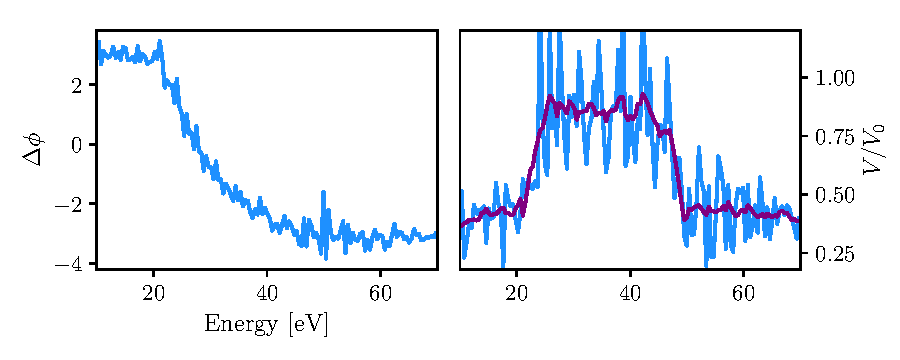
\includegraphics[width=1.0\textwidth]{figures/refractive_index/FTS_delta.pdf}
	\caption[Measured phase shift using SWPG FTS in silicon]{Spectral phase shift extracted from interferograms shown in figure \ref{fig:interferogram_si}. Phase shift is induced by the Si sample.}
	\label{fig:FTS_phase_si}
\end{figure}

\begin{figure}
	\centering
	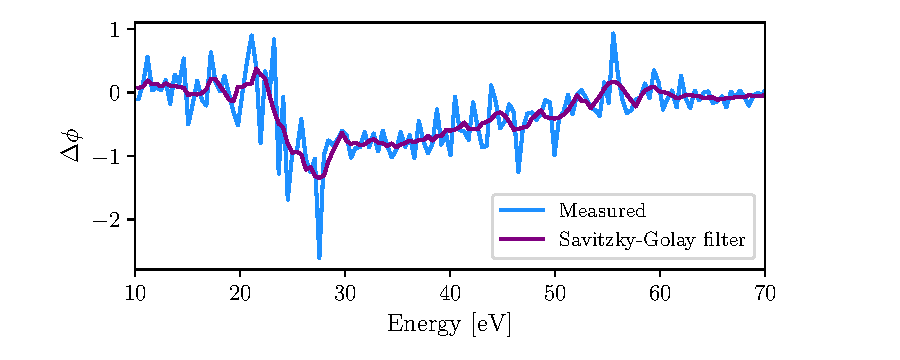
\includegraphics[width=1.0\textwidth]{figures/refractive_index/FTS_delta_ge.pdf}
	\caption[Measured phase shift using SWPG FTS in germanium]{Spectral phase shift extracted from interferograms shown in figure \ref{fig:interferogram_ge}. Phase shift is induced by the Ge sample.}
	\label{fig:FTS_phase_ge}
\end{figure}

From the interferograms shown in figures \ref{fig:interferogram_si} and \ref{fig:interferogram_ge}, it is possible extract the spectrally dependent phase shift that is imparted by the sample.  This is possible because those inteferograms constitute a Fourier-transform spectroscopy (FTS) measurement in the XUV using two phase locked beams generated by a SWPG.  FTS enables measurement of both the real and imaginary parts of the refractive index, however it is difficult to perform in the XUV because of technical requirements set by the available optics and because the intrinsically short wavelengths in this energy range require high interferometric stability and precise control over the relative delay between the interfering beams \cite{jansenSpatiallyResolvedFourier2016, jansenBroadbandExtremeUltraviolet2019, kovacevExtremeUltravioletFourierTransform2005, deoliveiraHighresolutionBroadbandwidthFouriertransform2011}.  Both of those difficulties are solved through the use of a SWPG to generate the two sources that are used in this measurement.  To extract the induced phase, the signal given by \ref{eqn:combined_spatialgram_theory} is Fourier transformed using the relative delay given by \ref{eqn:phase_to_delay}, and this yields
\begin{equation}
	\label{eqn:spatialgram_theory_FT}
	\tilde{S}(\omega) = A_{\mathrm{sample}}A_{\mathrm{ref}}\exp\big(i\Delta\Phi(\omega)\big).
\end{equation}
In principle, the phase $\Delta\Phi$ includes geometric phase variations and phase variations from the HHG process \cite{jansenBroadbandExtremeUltraviolet2019}.  To remove these contributions, a reference interferogram should be taken to isolate the phase contribution from the sample of interest, and this is precisely what was done by scanning the SWPG in the two positions mentioned previously.  The sample induced phase $\Delta\phi$ is calculated from \ref{eqn:spatialgram_theory_FT} for both positions through the relationship
\begin{equation}
	\label{eqn:measured_spectral_phase}
	\Delta\phi(\omega) = \arg\big[ \tilde{S}_{1}(\omega) \tilde{S}_{2}^{\ast}(\omega) \big]
\end{equation}
where $\tilde{S}_{1}(\omega)$ is the Fourier transformed interferogram measured at a position where only one source is on the sample and $\tilde{S}_{2}^{\ast}(\omega)$ the complex conjugate of the Fourier transformed interferogram measured at a position where neither source is on the sample of interest \cite{jansenBroadbandExtremeUltraviolet2019}.  This analysis was performed to extract the phase shift induced by the Si and Ge samples shown in figure \ref{fig:split_sample}, and the resulting phase shift is shown in figure \ref{fig:FTS_phase_si} (a) for the Si sample and figure \ref{fig:FTS_phase_ge} (a) for the Ge sample.  The phase induced by the Si sample shows a decreasing phase shift as the energy is increased with no apparent resonant structure, and this is expected for Si because there are no absorption edges corresponding to a core-level transition in this energy range \cite{henkeXRayInteractionsPhotoabsorption1993}.  The phase shift induced by the Ge sample, on the other hand, shows a pronounced resonance feature around 30 eV.  This feature can be assigned to the $M_{4,5}$ absorption edge due to a core-level transition from the $3d$ states to states in the vicinity of the Fermi energy \cite{henkeXRayInteractionsPhotoabsorption1993, kaplanRetrievalComplexvaluedRefractive2019, borjaExtremeUltravioletTransient2016, krausAttosecondTransientReflectivity2016, zurchDirectSimultaneousObservation2017, zurchUltrafastCarrierThermalization2017}. The signal is noisier in this case when compared to the Si sample because of the overall lower sample quality and the comparatively weaker harmonics in this energy range because of the absorption resonance and absorption from the substrate which does not contribute to the measured phase.  This could be improved by fabricating a thinner sample with a more step-like thickness profile on a thinner membrane or by fabricating a free-standing membrane of Ge similar to the Si sample.


Beyond the sample induced phase shift, FTS can also give access to the imaginary part of the refractive index and thereby the energy dependent transmission of the sample.  This can be calculated from the interferograms at the two positions along the sample using the relationship
\begin{equation}
	\label{eqn:transmission_s1_s2}
	\begin{aligned}
		T(\omega) &= \frac{A_{\mathrm{sample}}(\omega)}{A_{\mathrm{ref}}(\omega)} = \frac{A_{\mathrm{sample}}(\omega)A_{\mathrm{ref}}(\omega)}{A_{\mathrm{ref}}(\omega)A_{\mathrm{ref}}(\omega)}\\
						&=\frac{\abs{\tilde{S}_1(\omega)}}{\abs{\tilde{S}_2(\omega)}}.
	\end{aligned}
\end{equation}
Applying this calculation to the interferograms measured for both samples is shown in figure \ref{fig:FTS_phase_si} (b) and \ref{fig:FTS_phase_ge} (b) for Si and Ge, respectively.  As can be seen from these figures, the transmission is noisier than the induced phase, however several features can still be observed in the energy range of 20-45 eV.  In the case of Si, there is an increasing transmission that plateaus as the energy is increased.  The drop is transmission past 45 eV is likely an artifact of the poor fringe contrast in the harmonics generated above 45 eV.  This general behaviour agrees well with what is expected for Si \cite{henkeXRayInteractionsPhotoabsorption1993}.  For the case of Ge, the signal is even noisier than that of Si, however there is still a drop on transmission at 30 eV that corresponds to the $M_{4,5}$ absorption edge.

\begin{figure}
	\centering
	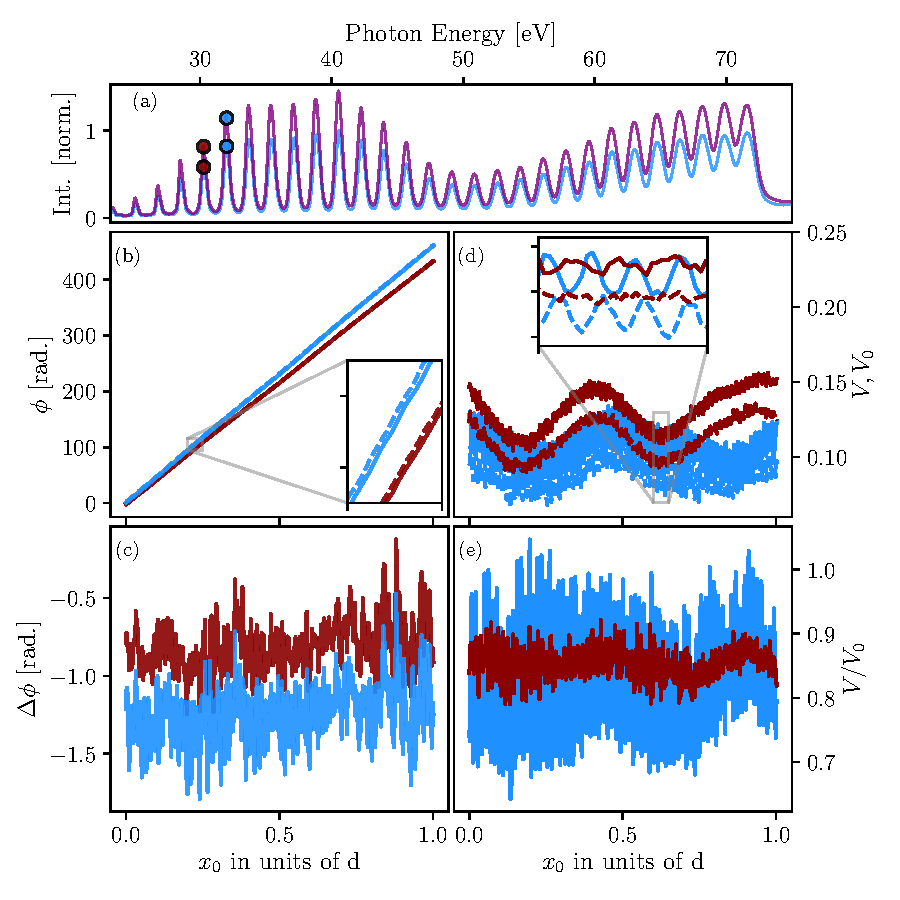
\includegraphics[width=1.0\textwidth]{figures/refractive_index/phase_fringe_extraction.pdf}
	\caption[Fringe shift and fringe  contrast extracted from SWPG scan]{(a) Reference harmonic spectrum showing the two harmonics of interest. (b) Phase of the spatial frequency corresponding to the two harmonics of interest. (c) Difference in phase between the positions along the sample thickness profile. (d) Fringe contrast of each harmonic for the two positions along the sample.  (e) Ratio of fringe contrast between the two positions.}
	\label{fig:phase_fringe_extraction}
\end{figure}

An additional way to extract the spectral phase and transmission induced by the sample is by examining the fringe shift and contrast as the grating position is varied in a similar manner as to what was done while the two samples were translated through the focus of the XUV, see figures \ref{fig:harmonic_phase_shift} and \ref{fig:harmonic_fringe_shift_contrast_ge}.  This can be done for each harmonic as $x_0$ is varied at the two positions along the sample thickness profile.  The resulting fringe shift and contrast can then be averaged to give a measurement of the induced phase shift and absorption of the sample across the harmonic spectrum.  This is shown for two harmonics in figure \ref{fig:phase_fringe_extraction}.  The phase $\phi$ corresponds to the phase of the spatial frequency of the harmonic, and it varies linearly with grating position $x_0$ via the relationship
\begin{equation}
	\phi=\bigg(q\frac{4\pi}{d}\bigg)x_0 + \phi_0.
\end{equation} 
As can be seen in the figure, the phase offset is different for the two positions where only one source is transmitting through the sample (solid line) and where neither sources are transmitting through (dashed line).  The difference in phase between these two cases is precisely the sample induced phase that measured previously by the FTS method, and the phase difference $\Delta\phi$ can be averaged over $x_0$ to give a more accurate phase shift at that harmonic energy. 

In a similar way to the fringe shift, the fringe contrast can be measured as the phase grating is translated for the two sample positions. The resulting fringe contrast is shown in figure \ref{fig:phase_fringe_extraction} (d) for the position where only one source transmits ($V$, dashed line) and where neither source does ($V_0$, solid line).  As expected, the fringe contrast is greater for the case where neither source transmits through the sample because of the differential nature of this measurement.  The modulations that are observed in the contrast as the SWPG is translated through the beam are due to interferences between the two sources in generation of the XUV beams.  The leakage of one IR source into the other causes the slower modulations with a period of $d/2$, and the higher frequency modulations are due to interferences between the two sources at the harmonic energy.  Regardless of their origin, the relevant quantity to extract the absorption induced by the sample is related to the ratio of contrasts $V/V_0$, see equation \ref{eqn:beta_fringe_contrast}, and averaging $V/V_0$ over $x_0$ gives a more accurate change in fringe contrast. 


Finally, we can now calculate both the real and imaginary part of the refractive index of Si and Ge over the range 25 - 60 eV by combining both the fringe shift and the change in fringe contrast and by using the FTS method.  The results are shown in figure \ref{fig:measured_delta_beta} for Si and figure \ref{fig:measured_delta_beta_ge} for Ge.  As can be seen in the figure \ref{fig:measured_delta_beta}, there is excellent agreement between the measured real and imaginary parts of the refractive index of Si when compared to the values that can be obtained from CXRO \cite{henkeXRayInteractionsPhotoabsorption1993}.  Both methods agree exceedingly well across most of the energy range of interest for the real part of the refractive index, however there are deviations between the FTS method (blue line) and the average fringe shift (purple dots) at energies above 45 eV.  This is most likely due to the poor fringe contrast at energies above 45 eV, as seen in figure \ref{fig:ref_img_spec} (a).  This deviation between the two methods is most pronounced in the imaginary part $\beta$ shown in figure \ref{fig:measured_delta_beta} (b).  In principle, this measurement can be improved by generating harmonics with good contrast over the entire energy range of interest, and this can most easily be accomplished by using a grating with a larger period to reduce the overall spatial frequencies.

\begin{figure}
	\centering
	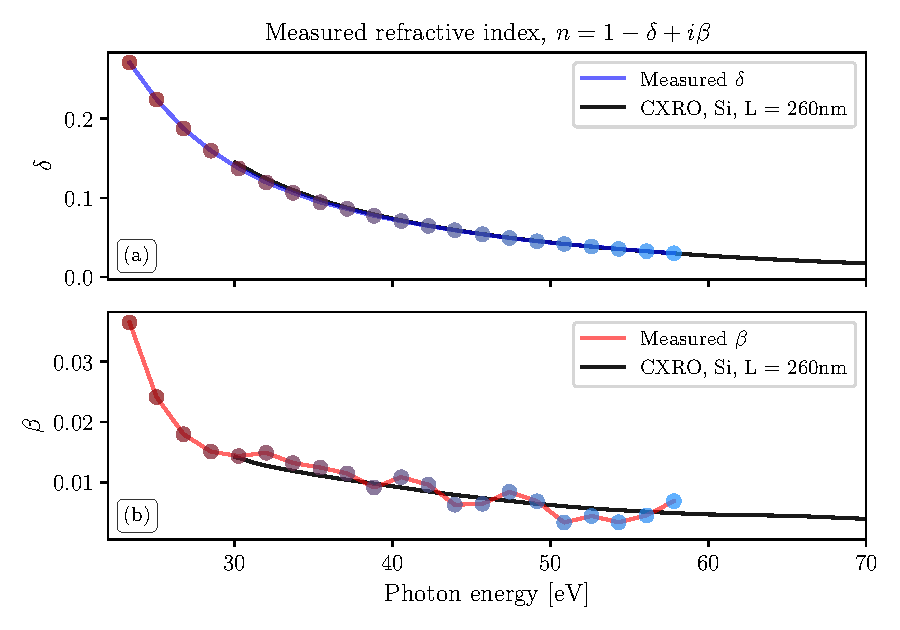
\includegraphics[width=0.9\textwidth]{figures/refractive_index/db_cxro.pdf}
	\caption[Measured real and imaginary part of the refractive index of Si using a SWPG]{Real (a) and imaginary (b) part of the refractive index of Si measured with a SWPG using FTS (blue line) and averaging fringe contrast (FC) and fringe shift (FS) over $x_0$ (purple dots).}
	\label{fig:measured_delta_beta}
\end{figure}

\begin{figure}
	\centering
	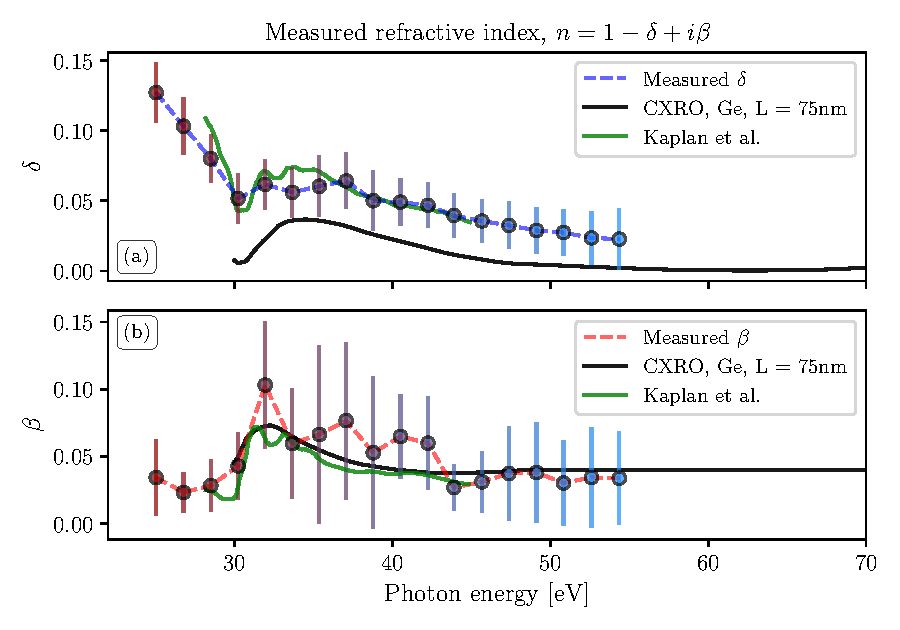
\includegraphics[width=0.9\textwidth]{figures/refractive_index/ge_refractive.pdf}
	\caption[Measured real and imaginary part of the refractive index of Ge using a SWPG]{Real (a) and imaginary (b) part of the refractive index of Ge measured with a SWPG using FTS (blue line) and averaging fringe contrast (FC) and fringe shift (FS) over $x_0$ (purple dots).}
	\label{fig:measured_delta_beta_ge}
\end{figure}

In this energy range, the Si refractive index is devoid of any resonance features because there no nearby absorption edges, so its measurement represents an easy benchmark of both methods of extracting the refractive index. However, what is typically of interest in most experiments is the refractive index at an absorption edge where there is strong variation in refractive index that is intrinsically related to the properties of the material in question.  This is where the measurement of the refractive index of Ge, as shown in figure \ref{fig:measured_delta_beta_ge}, comes in to play.  As mentioned previously, the $M_{4,5}$ absorption edge in Ge is located at 30 eV, and its presence causes a large increase in absorption and a modulation of the phase around the absorption edge.  The refractive index that has been tabulated by CXRO generally is only accurate far from such resonance features. However, recent measurements of the refractive index were performed by Kaplan, \emph{et. al.} \cite{kaplanRetrievalComplexvaluedRefractive2019}, and this measurement serves as a good comparison to the two measurements methods presented herein.  As can be seen from figure \ref{fig:measured_delta_beta_ge}, there is generally excellent agreement between the two measurement methods and  Kaplan, \emph{et. al.} for the real part of the refractive index over the entire energy range of interest, however there are small deviations just above the edge between them. In this energy range just above the edge, the material properties of the sample strongly influence the refractive index, and further study of the sample properties could explain the deviations \cite{kaplanRetrievalComplexvaluedRefractive2019, stohrNEXAFSSpectroscopy1992, attwoodSoftXraysExtreme2000}.  Similarly to the real part of the refractive index, the imaginary part, see figure \ref{fig:measured_delta_beta_ge} (b), shows good overall agreement from 30 - 45 eV in the vicinity of the absorption edge with small deviations that could possibly be explained with further analysis.  However, for the imaginary part, the FTS fails outside the energy range of 30-45 eV because of a noisy signal.  This could be improved both by fabricating a higher quality sample with a more suitable thickness profile and by optimizing the harmonics for better contrast over a larger energy.  Regardless, this demonstrates the feasibility of using a SWPG to measure the complex refractive index over a large energy range in a single measurement even when a resonant feature is present.



\section{Conclusion}
In this chapter, the complex refractive index was introduced and a method to measure both the real and imaginary parts was proposed. The method relies on the use of a $0-\pi$ SWPG to generate two relative phase locked XUV sources whose interference acts as an inline Mach-Zehnder interferometer.  By introducing a sample into one of the sources, the corresponding fringe shift and change in fringe contrast gives access to the real and imaginary parts of the refractive index. The intrinsic phase control offered by the SWPG allows for FTS to be performed by varying the SWPG position within the beam. Samples of Si and Ge were fabricated to test this method, and measuring their refractive index shows excellent agreement between our measured results and the literature. Thus, we have demonstrated the capability of using a SWPG to characterize the ground state complex refractive index of a condensed matter system.  The next step is to extract the dynamic real and imaginary parts that are induced by dressing the sample with another IR field.  This will be discussed in a later chapter.




\chapter{Attosecond Transient-absorption Spectroscopy}
\label{chap:ATS}

\section{Introduction}
\label{sec:intro_ats}


\section{Autoionization resonances}
\label{sec:fano_ar}

One of the most extensively studied phenomenons using ATS has been autoionization of noble gas atoms in the time-domain \cite{wangAttosecondTimeResolvedAutoionization2010, ottAttosecondMultidimensionalInterferometry2012, stoossRealTimeReconstructionStrongFieldDriven2018, kaldunExtractingPhaseAmplitude2014, kaldunObservingUltrafastBuildup2016}.  Autoionization was first observed in 1935 by Beutler \cite{beutlerUeberAbsorptionsserienArgon1935} by studying photoabsorption of noble gas atoms, and it manifested itself as sharp, asymmetric peaks in the absorption spectrum.  These features were theoretically described by Fano in a seminal paper in 1961 \cite{fanoSulloSpettroDi1935, fanoEffectsConfigurationInteraction1961} as the result of interference between two pathways: direct ionization to the continuum and autoionization from a discrete state that is embedded in and coupled to the continuum. The theoretical framework that he developed can be treated as a more general formalism that describes interference between discrete and continuous pathways.\footnote{A very similar theory was independently developed by Feshbach in the context of nuclear physics, and these two theories have been unified by further theoretical work \cite{feshbachUnifiedTheoryNuclear1958, feshbachUnifiedTheoryNuclear1962, bhatiaLineshapeParameters1P1984}
	.} For this very reason, "Fano" resonances can be observed in a plethora of atomic, molecular, and condensed matter systems \cite{miroshnichenkoFanoResonancesNanoscale2010}.

\subsection{Autoionization in the frequency domain: Fano's original work}
\label{sec:og_fano}

As noted above, Fano's theoretical explanation of the photoabsorption spectrum observed by Beutler in noble gas atoms is based on interference between two pathways.  The relevant level diagram to describe this scenario is shown in figure \ref{fig:fano_level_diagram}, and specifically we will be considering the autoionization resonances in Ar because they will be used in the ATS experiments described in this chapter and in the following chapter.  In this case, there is a bound state $\ket{\psi_b}$ (one of the $3s3p^6np$ states in Ar) that is embedded within a set of continuum states $\ket{\psi_\varepsilon}$.  This entails that the energy of the bound state $E_b$ is degenerate with the energetic spectrum of continuum states. The coupling between the bound state $\ket{\psi_b}$ and the continuum $\ket{\psi_\varepsilon}$ through the configuration interaction leads to decay of the electron from the bound state to the continuum.  The following derivation of the photoabsorption cross section and phase follows closely from Fano's original paper and sources that have reproduced his original derivation \cite{fanoEffectsConfigurationInteraction1961, changFundamentalsAttosecondOptics2011, ottAttosecondMultidimensionalInterferometry2012}.

\begin{figure}
	\centering
	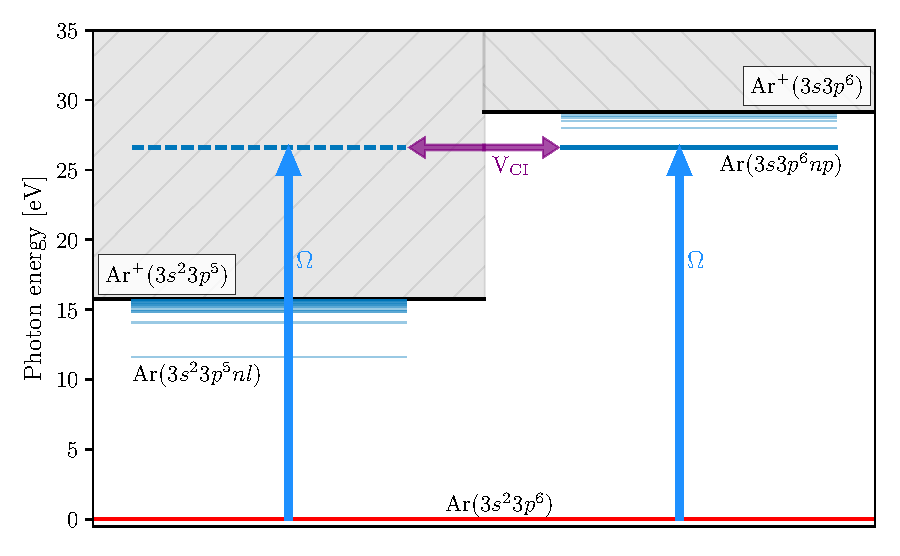
\includegraphics[width=0.8\textwidth]{figures/ATS/fano_level_diagram.pdf}
	\caption[Level diagram of Fano resonances in Argon]{Level diagram of argon showing the effect of autoionization states on XUV photoabsorption. There are two possible pathways for ionization with a photon of energy $\Omega$: (1) direct ionization to a continuum state (left side of figure) and (2) excitation to a bound state in the continuum (right side of figure).  In case (2), there is coupling between the bound state and the continuum through the configuration interaction.  This allows for the bound state to decay to the same continuum state as in case (1).  These effect leads to interference between these two pathways.}
	\label{fig:fano_level_diagram}
\end{figure}

The Hamiltonian describing this system can  be written as
\begin{equation}
\label{eqn:hamiltonian}
	\hat{H} = \hat{H_0} + \hat{V},
\end{equation}
where $\hat{H_0}$ is the zeroth order Hamiltonian and $\hat{V}$ is the correlation potential that describes the coupling between the discrete state $\ket{\psi_b}$ and the continuum state $\ket{\psi_\varepsilon}$.  The solutions to the zeroth order Hamiltonian are the continuum and bound states, such that 
\begin{align}
\label{eqn:configurations_hamiltonian}
	\hat{H_0}\ket{\psi_b} &= E_b\ket{\psi_b}\\
	\hat{H_0}\ket{\psi_\varepsilon} &= \varepsilon\ket{\psi_\varepsilon}
\end{align}
where the states $\ket{\psi_b}$ and $\ket{\psi_\varepsilon}$ are orthonormal.  These two solutions to the zeroth order Hamiltonian are referred to as configurations, and the interaction between them is given by $\hat{V}$. The coupling strength between these two configurations is given by the off-diagonal matrix element $V_\varepsilon$, such that
\begin{equation}
\label{eqn:coupling_matrix_element}
	\braket{\psi_\varepsilon|\hat{H}|\psi_b} = \braket{\psi_\varepsilon|\hat{H_0}+\hat{V}|\psi_b} = \braket{\psi_\varepsilon|\hat{V}|\psi_b} = V_\varepsilon.
\end{equation}  
This configuration interaction matrix element $V_\varepsilon$ depends upon the energy $\varepsilon$ and is generally a smooth function of the continuous energy $\varepsilon$.  Furthermore, the configuration interaction only couples different configurations and not within the same configuration.  The means that the diagonal matrix elements of $\hat{V}$ are zero,
\begin{align}
\label{eqn:config_int_diagonal}
	\braket{\psi_\varepsilon|\hat{V}|\psi_\varepsilon} &=0\\
	\braket{\psi_b|\hat{V}|\psi_b} &=0.
\end{align}
Therefore, the diagonal matrix elements of the full Hamiltonian in equation \ref{eqn:hamiltonian} are given by
\begin{align}
	\braket{\psi_\varepsilon|\hat{H}|\psi_\varepsilon} &= \varepsilon\delta(\varepsilon-\varepsilon')\\
	\braket{\psi_b|\hat{H}|\psi_b} &= E_b. 
\end{align}

Armed with these states as a basis, we can now expand an eigenstate of the full Hamiltonian $\hat{H}$.  This entails that the eigenstate $\ket{\Psi_E}$ of energy $E$, which is found by solving the equation
\begin{equation}
	\hat{H}\ket{\Psi_E}=E\ket{\Psi_E},
\end{equation}
can be expanded in this complete basis, such that
\begin{equation}
\label{eqn:eigenstate_expansion}
	\ket{\Psi_E} = a(E)\ket{\psi_b} + \int\diff\varepsilon'b(\varepsilon',E)\ket{\psi_{\varepsilon'}}.
\end{equation}
The physical interpretation of this expansion is that an electron at energy $E$ can originate from either the discrete state $\ket{\psi_b}$ or from the continuous state $\ket{\psi_\varepsilon}$.  The contribution from $\ket{\psi_\varepsilon}$ is direct ionization, and the contribution from $\ket{\psi_b}$ is autoionization (i.e. decay from the bound state $\ket{\psi_b}$ to the continuum).  The relative contributions of these two channels is given by the expansion coefficients $a(E)$ and $b(\varepsilon,E)$.

These expansion coefficients can be solved for and it involves algebra that is described in full detail in Fano's paper \cite{fanoEffectsConfigurationInteraction1961}.  The first step is to evaluate the relationship
\begin{equation}
	\braket{\Psi_E|\hat{H}|\Psi_E} = E
\end{equation}
using the expansion in eqn. \ref{eqn:eigenstate_expansion}.  This results in a system of two equations with the unknown coefficients $a(E)$ and $b(\varepsilon,E)$.  This system can be solved for analytical expressions of the expansion coefficients, and they are given by
\begin{align}
\label{eqn:expansion_coeff_a}
	a(E) &= \frac{\sin\Delta(E)}{\pi V_E}\\
\label{eqn:expansion_coeff_b}
	b(\varepsilon',E) &= \frac{V_{\varepsilon'}}{E-\varepsilon'}a(E)-\delta(\varepsilon'-E)\cos\Delta(E)
\end{align}
where
\begin{align}
\label{eqn:expansion_coeff_delta}
	\Delta(E) &= -\arctan\bigg(\frac{\pi\lvert V_E \rvert^2}{E-E_b-F(E)}\bigg)\\
\label{eqn:expansion_coeff_delta_F}
	F(E) &= \mathrm{PV}\int\diff\varepsilon'\frac{\lvert V_{\varepsilon'}\rvert^2}{E-\varepsilon'} 
\end{align}
and $\mathrm{PV}$ is the Cauchy principal value. The term  $F(E)$ is an energy-dependent shift of the bound state that depends upon the strength of the configuration interaction $\abs{V_{\varepsilon'}}^2$.  This shift can be either positive or negative, depending upon the sign of $\partial_{\varepsilon'}\abs{V_{\varepsilon'}}^2$ at $\varepsilon'=E$, where $\partial_{\varepsilon'}$ is the partial derivative with respect to $\varepsilon'$.  Thus, any change in  $V_{\varepsilon'}$ by an external field will lead to a shift in the resonance position.

Substituting the coefficients in equations \ref{eqn:expansion_coeff_a} and \ref{eqn:expansion_coeff_b} into equation \ref{eqn:eigenstate_expansion} yields
\begin{equation}
	\ket{\Psi_E}=\frac{\sin\Delta(E)}{\pi V_E}\ket{\psi_b}+\frac{\sin\Delta(E)}{\pi V_E}\bigg(\mathrm{PV}\int\diff\varepsilon'\frac{V_{\varepsilon'}}{E-\varepsilon'}\bigg)\ket{\psi_\varepsilon'}-\cos\Delta(E)\ket{\psi_E}.
\end{equation}
This can be further simplified by  introducing a modified discrete state given by
\begin{equation}
	\ket{\Phi} = \ket{\psi_b}+\mathrm{PV}\int\diff \varepsilon'\frac{V_\varepsilon'}{E-\varepsilon'}\ket{\psi_{\varepsilon'}},
\end{equation}
which allows us to express the eigenstate $\ket{\Psi_E}$ as
\begin{equation}
\label{eqn:eigen_with_a_b}
	\ket{\Psi_E}=\frac{\sin\Delta(E)}{\pi V_{E}}\ket{\Phi} - \cos\Delta(E)\ket{\psi_E}.
\end{equation}
Finally, the argument of equation \ref{eqn:expansion_coeff_delta_F} can be written in terms of an important parameter, the reduced energy given by
\begin{equation}
\label{eqn:normalized_eng}
	\epsilon = \frac{E-(E_b+F(E))}{\Gamma(E)/2} = \frac{E-E_\Phi}{\Gamma/2}
\end{equation}
where
\begin{equation}
	\Gamma(E) = 2\pi\abs{V_E}^2\approx\Gamma(E_b)=\Gamma.
\end{equation}
The interpretation of the modified bound state $\ket{\Phi}$ is that the configuration interaction is mixing the original discrete state $\ket{\psi_b}$ and the continuum states $\ket{\psi_\varepsilon'}$. So, for an energetic window near $E=E_\Phi$, one can consider the resonance energy to be $E_b$ and the resonance linewidth to be $\Gamma$.  Since $\Gamma=2\pi\abs{V_E}^2$, the resonance linewidth and the natural lifetime $h/\Gamma$ are directly related to the strength of the coupling between bound states and continuum states though the configuration interaction. Therefore, stronger (weaker) coupling would lead to faster (slower) decay from bound to continuum states, respectively.  From this, it can be seen that an external field that  is able to modify the strength of the configuration interaction, then that will lead to a change in the linewidth and position of the resonance.

Now that the eigenstates of the Hamiltonian $\hat{H}$ have been expanded, we will turn our attention to the photoabsorption spectrum.  In the original experiments done by Beutler, a sharp, asymmetric absorption profile was seen in the photoabsorption spectrum of noble gas atoms in the XUV \cite{beutlerUeberAbsorptionsserienArgon1935}.  From the expanded eigenstate given in equation \ref{eqn:eigen_with_a_b}, we can begin see how this asymmetric absorption profile might arise.  The coefficients in the expansion are proportional to sine and cosine functions of the reduced energy $\epsilon$, and, since they are odd and even functions of $\epsilon$, this will lead to constructive and destructive interference on either side of the resonance.  It is precisely this effect that will give rise to the asymmetric absorption lineshape.

To derive the photoabsorption spectrum, we will consider a transition from the ground state of the atom $\ket{g}$ by a XUV photon of energy $\Omega$.  This can be described through the use of the dipole transition operator
\begin{equation}
\label{eqn:dipole}
	\hat{D}=-e\mathbf{\hat{r}}\cdot\mathbf{E}_{XUV}(t)
\end{equation}
where $\mathbf{E}_{XUV}(t)$ is the electric field of the XUV.  Using this operator, the transition probability is given by the matrix element
\begin{equation}
\label{eqn:transition_me}
	\begin{aligned}
		\braket{\Psi_E|\hat{D}|g} &= \frac{1}{\pi V^*_{E}}\sin\Delta(E)\braket{\Phi|\hat{D}|g}-\cos\Delta(E)\braket{\psi_E|\hat{D}|g}\\
		&= \cos\Delta(E)\braket{\psi_E|\hat{D}|g}\Bigg[\tan\Delta(E)\frac{1}{\pi V^*_E}\frac{\braket{\Phi|\hat{D}|g}}{\braket{\psi_E|\hat{D}|g}} -1\Bigg].
	\end{aligned} 
\end{equation}
At this point, we can now introduce the well-known and important $q$ parameter, given by
\begin{equation}
\label{eqn:q-parameter}
	q(E) = \frac{1}{\pi V^*_E}\frac{\braket{\Phi|\hat{D}|g}}{\braket{\psi_E|\hat{D}|g}}\approx q(E_b)=q.
\end{equation}
The $q$ parameter describes the asymmetry of the resonance, and it is related to the ratio of transitions to the modified bound state $\ket{\Phi}$ and the continuum states $\ket{\psi_E}$.  Combining equations \ref{eqn:transition_me}, \ref{eqn:q-parameter}, and \ref{eqn:expansion_coeff_delta}, we arrive at
\begin{align}
	\braket{\Psi_E|\hat{D}|g} &=-\cos\Delta(E)\braket{\psi_E|\hat{D}|g}\Bigg[\frac{\pi\abs{V_E}^2}{E-(E_b+F(E))}q+1\Bigg]\\
	&=-\cos\Delta(E)\braket{\psi_E|\hat{D}|g}\Bigg[\frac{\Gamma/2}{E-(E_b+F(E))}q+1\Bigg],
\end{align}
and this can be further simplified using the reduced energy $\epsilon$, which yields
\begin{align}
	\braket{\Psi_E|\hat{D}|g} &= -\braket{\psi_E|\hat{D}|g}\cos\Delta(E)\bigg(\frac{q}{\epsilon}+1\bigg)\\
\label{eqn:fano_matirx_elements}
	\braket{\Psi_E|\hat{D}|g} &= \braket{\psi_E|\hat{D}|g}\frac{q+\epsilon}{\epsilon+i}.
\end{align}
Finally, using this relationship the ratio of transition probabilities can be calculated and leads to the well known Fano lineshape,
\begin{equation}
\label{eqn:transition_prob_ratio}
	\frac{\abs{\braket{\Psi_E|\hat{D}|g}}^2}{\abs{\braket{\psi_E|\hat{D}|g}}^2}=\frac{(q+\epsilon)^2}{\epsilon^2 + 1}.
\end{equation}
This ratio is proportional to the photoabsorption cross section, and is plotted for various $q$ parameters in figure \ref{fig:cross_sec_and_phase}.  As can be seen, the lineshape's symmetry dramatically depends upon the $q$ parameter, and the cross section even goes to zero at different energies, depending upon $q$. This is a direct consequence of the destructive interference from the configuration states, as was predicted earlier in the derivation. Additionally, the spectral phase of the Fano profile can also be extracted, given by 
\begin{equation}
	\theta(\epsilon)=\arg\bigg[\frac{q+\epsilon}{\epsilon+i}\bigg],
\end{equation}
and is plotted in figure \ref{fig:cross_sec_and_phase} (b).  For increasing $\epsilon$, the phase increases until $\epsilon=-q$ when there is a $\pi$ phase jump, and thereafter the phase continues to increase until is asymptotically approaches its original value.
\begin{figure}
	\centering
	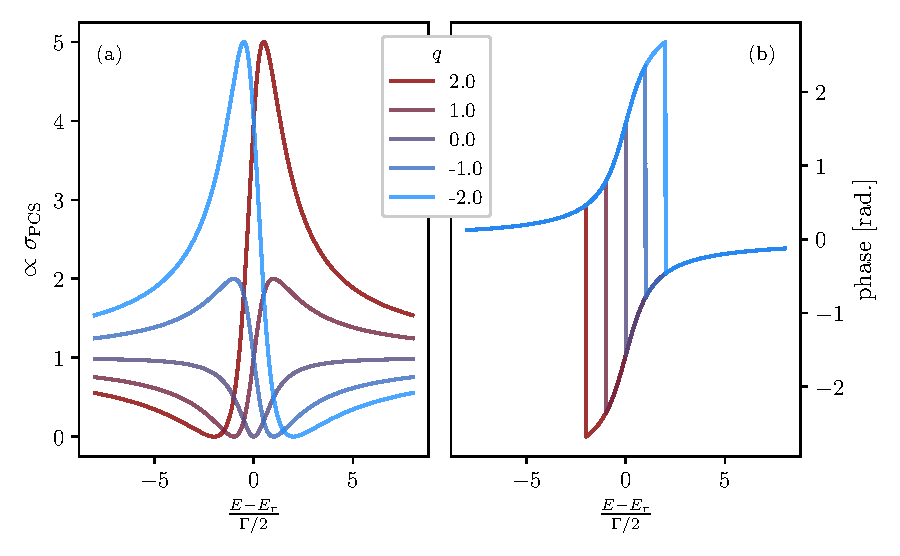
\includegraphics[width=0.8\textwidth]{figures/ATS/cs_phase.pdf}
	\caption[Photoabsorption cross section and phase of a Fano resonance]{(a) Calculation of the photoabsorption cross section near a resonance for the listed $q$ parameters.  The change from symmetric to asymmetric profiles can be seen as the $q$ parameter is varied. Maximum and minimum in cross section occus at $\epsilon=1/q$ and $\epsilon=-q\Gamma^2/4$, respectively. (b) Calculation of the phase across the resonance for different $q$ parameter. The $\pi$ phase jump clearly depends on $q$, and it occurs when $\epsilon=-q$ and not at the resonance energy $E_r$. Calculations based on U. Fano's original work \cite{fanoEffectsConfigurationInteraction1961}.}
	\label{fig:cross_sec_and_phase}
\end{figure}

Experimentally the photoabsorption cross section is generally fit to the form
\begin{equation}
\label{eqn:sigma_pcs}
	\sigma_\mathrm{PCS}=\sigma_a\frac{(q+\epsilon)^2}{\epsilon^2+1}+\sigma_{NR}
\end{equation}
where $\sigma_a$ scales the strength of the Fano profile and $\sigma_{NR}$ is  a non-resonant cross section that is included to account for absorption from  other continuum states that might be present.  



\subsection{Autoionization in the time domain}
\label{sec:time_dependent_autoionization}
%
%!!!!!!!!!!!!!!!!!!!!!!!!!!!!!!!!!!!!!!!!!!!!!!!!!!!!!!!!!!!!!!!!!!!!!!!!!!!!!!!!!
%!!!!!!!!!!!!!!!!!!!!!!!!!!! ATOMIC UNITS !!!!!!!!!!!!!!!!!!!!!!!!!!!!!!!!!!!!!!!!
%!!!!!!!!!!!!!!!!!!!!!!!!!!!!!!!!!!!!!!!!!!!!!!!!!!!!!!!!!!!!!!!!!!!!!!!!!!!!!!!!!
%

Up until this point, Fano resonances have been discussed in a time-independent manner in the frequency domain.  However, one would ideally like to describe these autoionizing resonances in the time domain, as that will lend itself to the experiments described herein. This description was primarily done by W.-C. Chu and C.D. Lin \cite{chuTheoryUltrafastAutoionization2010}, and it has been used to interpret many ATS experiments  \cite{kaldunExtractingPhaseAmplitude2014,ottLorentzMeetsFano2013,ottReconstructionControlTimedependent2014, stoossRealTimeReconstructionStrongFieldDriven2018}.  The basic assumption that is made in this treatment is that the XUV pulse that excites from the ground state to the Fano resonance is a Dirac-$\delta$ function in time, $\mathbf{E}_{XUV}=E_0\delta(t)\mathbf{z}$.  This impulsive excitation is generally a reasonable  approximation for an attosecond XUV pulse that is shorter in duration than the typical lifetimes of these resonances.  From this assumption, it is possible to analytically describe the dipole response of the system in the time domain.


The derivation of the dipole response follows naturally from the theory described in the previous section. Assuming that the XUV impulsively excites at $t=0$ from the ground state $\ket{g}$ to the bound and continuum states $\ket{\psi_b}$ and $\ket{\psi_\varepsilon}$, the wave function for times $t>0$ can be in the configuration states, such that
\begin{equation}
\label{eqn:wvfnc_expansion}
	\ket{\Psi(t)}=e^{-i\varepsilon_gt}\ket{g}+c_b(t)\ket{\psi_b}+\int c_\varepsilon(t)\ket{\psi_\varepsilon}\diff \varepsilon.
\end{equation}
Since the configuration states $\ket{\psi_b}$ and $\ket{\psi_\varepsilon}$ are not eigenstates of the total Hamiltonian, the expansion coefficients $c_b$ and $c_\varepsilon$ are explicitly time dependent. The evolution of these coefficients is governed by the Time-Dependent Schr{\"o}dinger Equation (TDSE)
\begin{equation}
\label{eqn:tdse}
	i\frac{\partial}{\partial t}\ket{\Psi(t)}=\hat{H}\ket{\Psi(t)},
\end{equation}
and using this equation, the time dependence of the expansion coefficients can be expressed as the coupled differential equations given by
\begin{equation}
\label{eqn:coupled_pde}
	\begin{aligned}
		\frac{\partial c_{\varepsilon}}{\partial t} &= -iV_\varepsilon c_b(t)-i\varepsilon c_\varepsilon(t)\\
		\frac{\partial c_b}{\partial t} &= -i\varepsilon_r c_b(t)-iV_\varepsilon \int c_\varepsilon(t) \diff \varepsilon.
	\end{aligned}
\end{equation}
Assuming the initial values $c_b^{(0)}$ and $c_\varepsilon^{(0)}$ are known, then the solutions to equations \ref{eqn:coupled_pde} are given by
\begin{equation}
\label{eqn:coefficients}
	\begin{aligned}
		c_b(t) &= c_b^{(0)}\bigg(1-\frac{i}{q}\bigg)e^{-i\varepsilon_r}e^{-\frac{\Gamma}{2}t}\\
		c_\varepsilon(t) &= \frac{c_\varepsilon^{(0)}}{\epsilon + i}e^{-i\varepsilon_r t}\bigg[ (q+\epsilon)e^{-i(\varepsilon-\varepsilon_r)t}-(q-i)e^{-\frac{\Gamma}{2}t}\bigg],
	\end{aligned}
\end{equation}
where, as in the previous section, $q=c_b^{(0)}/(\pi V c_\varepsilon^{(0)})$, $\Gamma=2\pi\rvert V \lvert^2$, and $\epsilon=(\varepsilon-\varepsilon_r)/(\Gamma/2)$. 


\begin{figure}
	\centering
	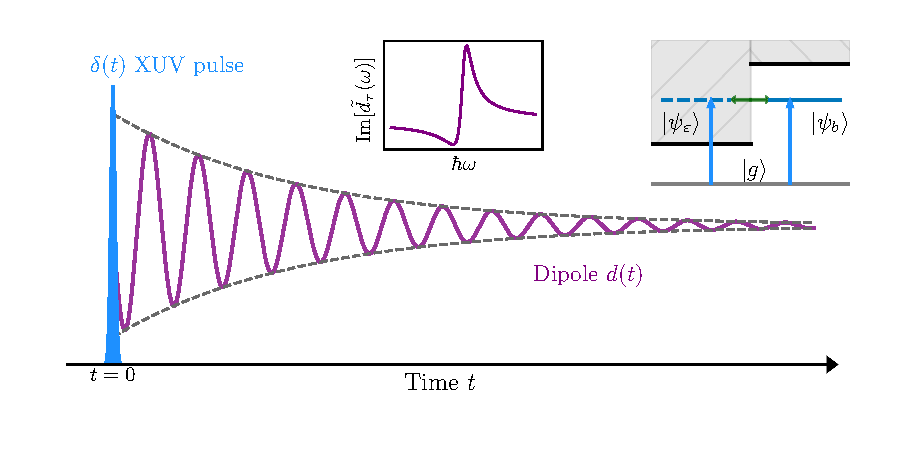
\includegraphics[width=1.0\textwidth]{figures/ATS/dipole_sketch.pdf}
	\caption[Illustration of dipole moment in the time-domain with various phase shifts]{Illustration of the dipole moment after a $\delta(t)$ excitation pulse. Dipole is shown for a phase shift of $\varphi=-1.2\pi$ (purple curve) and $\varphi=0$ (dashed gray curve), and the central inset shows the line shape for these two phase shifts.}
	\label{fig:dipole_sketch}
\end{figure}

With the time dependent wave function now in hand, the induced dipole $d(t)$ can now be calculated for $t>0$ by evaluating  $d(t)=\braket{\Psi(t)|z|\Psi(t)}$.  Using equations \ref{eqn:wvfnc_expansion} and \ref{eqn:coefficients}, this gives
\begin{equation}
\label{eqn:dip}
	\begin{aligned}
		d(t)&=c_b(t)e^{-i\varepsilon_g t}\braket{\psi_b|z|g}^* + \int c_\varepsilon(t)e^{i\varepsilon_g t}\braket{\psi_\varepsilon|z|g}^* + c.c.\\
		&=c_b^{(0)}\braket{\psi_b|z|g}^*e^{-i\Omega_r t}\Bigg[\bigg(1-\frac{i}{q}\bigg)e^{-\frac{\Gamma}{2}t}+ \frac{1}{(\pi V q)^2}\int \frac{(q+\epsilon)e^{-i\frac{\Gamma}{2}\epsilon t}-(q-i)e^{\frac{\Gamma}{2}t}}{\epsilon+i}\diff\varepsilon\Bigg] + c.c.,
	\end{aligned}
\end{equation}
where $\Omega_r=E_r-E_g$ is the resonance photon energy.  The complex conjugate term in equation \ref{eqn:dip} is a counter-rotating term, and by invoking the rotating wave approximation, it can be dropped.  Equation \ref{eqn:dip} can further be evaluated to give
\begin{equation}
	\begin{aligned}
	d(t) &= c_b^{(0)}\braket{\psi_b|z|g}^*e^{-i\Omega_r t}\frac{1}{q^2}\Bigg[q(q-i)e^{-\frac{\Gamma}{2}t}+\frac{2}{\pi\Gamma}\int \frac{(q+\epsilon)e^{-i\frac{\Gamma}{2}\epsilon t}-(q-i)e^{\frac{\Gamma}{2}t}}{\epsilon+i}\diff\varepsilon\Bigg]\\
	&= c_b^{(0)}\braket{\psi_b|z|g}^*e^{-i\Omega_r t}\frac{1}{q^2}\Bigg[q(q-i)e^{-\frac{\Gamma}{2}t} + \frac{1}{\pi} \int e^{-i\frac{\Gamma}{2}\epsilon t}\diff\epsilon + \frac{q-i}{\pi}\int \frac{e^{-i\frac{\Gamma}{2}\epsilon t} - e^{-\frac{\Gamma}{2}t}}{\epsilon+i} \diff\epsilon\Bigg]\\
	&=c_b^{(0)}\braket{\psi_b|z|g}^*e^{-i\Omega_r t}\frac{1}{q^2} \Bigg[ q(q-i)e^{-\frac{\Gamma}{2}t}+ \frac{4}{\Gamma}\delta(t) + \frac{q-i}{\pi}e^{-\frac{\Gamma}{2}t}2\pi i + \frac{q-i}{\pi}e^{-\frac{\Gamma}{2}t}\pi i \Bigg]\\
	&=c_b^{(0)}\braket{\psi_b|z|g}^*\frac{1}{q^2}\bigg[ \frac{4}{\Gamma}\delta(t)+(q-i)^2e^{-i\Omega_r t}e^{-\frac{\Gamma}{2}t}\bigg].
	\end{aligned}
\end{equation}
If we assume that $\braket{\psi_b|z|g}$ is real and the expansion coefficient is $c_b^{(0)}$ purely imaginary, then we can finally arrive at the form of the dipole that is reported in \cite{chuTheoryUltrafastAutoionization2010,ottLorentzMeetsFano2013,kaldunFanoResonancesTime2014},
\begin{equation}
\label{eqn:dipole_time_domain}
	d(t)\propto i\bigg[ 2\delta(t) + \frac{\Gamma}{2}(q-i)^2 e^{-i\Omega_r t}e^{\frac{\Gamma}{2}t} \bigg].
\end{equation}
This form of the dipole can be understood intuitively as arising naturally from the two interfering processes that are occurring: direct ionization to the continuum and decay from a discrete state to the continuum with a lifetime of $\hbar/\Gamma$.  The first $\delta$-function in equation \ref{eqn:dipole_time_domain} represents direct ionization, and the second term represents decay from the discrete state.  A schematic of the dipole after an impulsive XUV pulse is shown in  figure \ref{fig:dipole_sketch}.  To demonstrate that this formulation of the dipole in the time domain is compatible with Fano's original derivation, the photoabsorption cross section can be evaluated by
\begin{equation}
\begin{aligned}
	\sigma&=\frac{2\omega}{\epsilon_0 c}\mathrm{Im}\bigg[\frac{\tilde{d}(\omega)}{\tilde{E}(\omega)}\bigg]\propto \mathrm{Im}\bigg[\int_{-\infty}^{\infty} d(t) e^{i\omega t} \diff t\bigg]\\
	&\propto\mathrm{Re}\bigg[1+\frac{\Gamma}{2}(q-i)^2\int_0^\infty e^{-\frac{\Gamma}{2}t}e^{i(\omega-\Omega_r)t}\bigg]\\
	&\propto\mathrm{Re}\bigg[1 + \frac{(q-i)^2}{1-i\epsilon}\bigg]\\
	& \propto \frac{(q+\epsilon)^2}{\epsilon^2 +1}.
\end{aligned}
\end{equation}
This is exactly the cross section in equation \ref{eqn:sigma_pcs} that was derived previously.

\begin{figure}
	\centering
	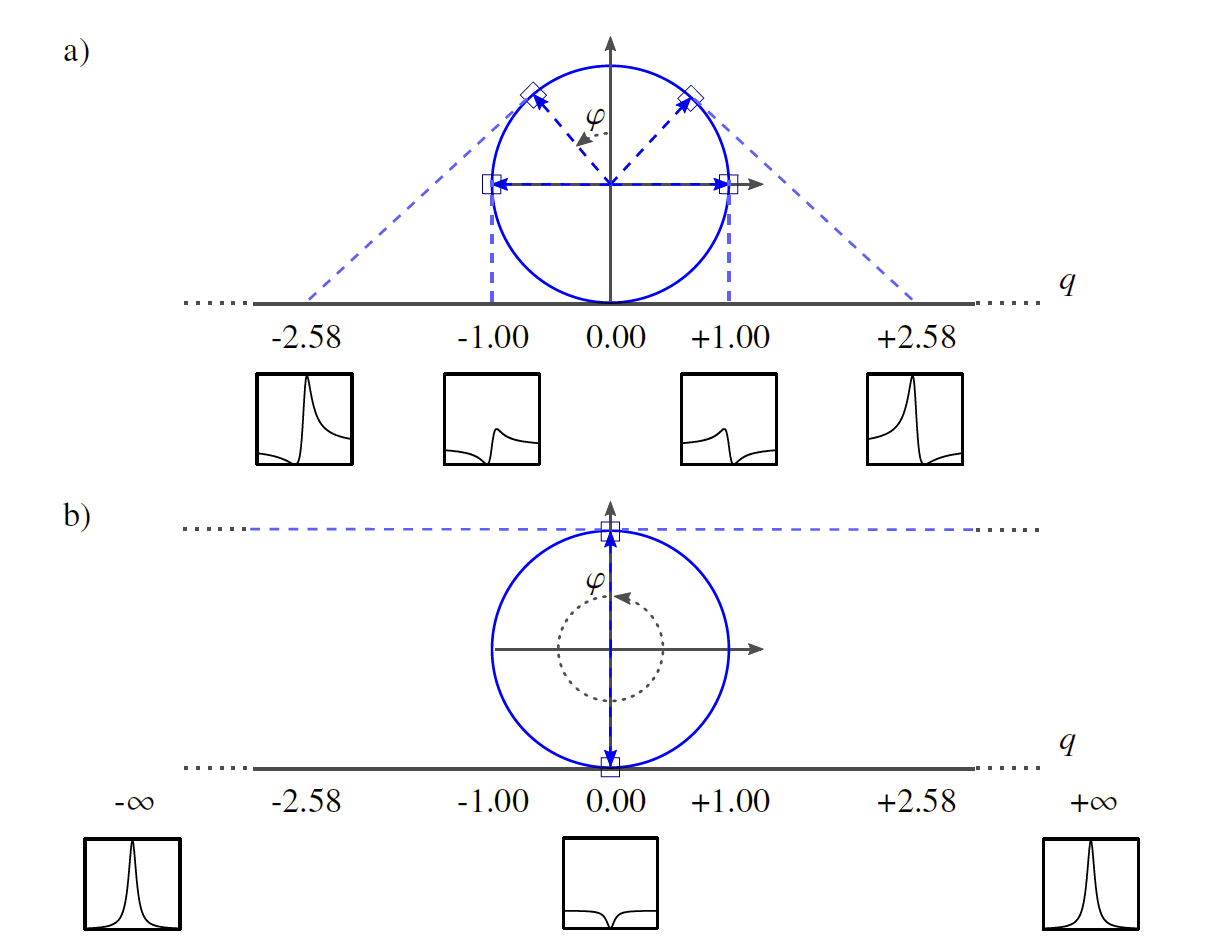
\includegraphics[width=0.8\textwidth]{figures/ATS/Kaldun.png}
	\caption[Illustration of the mapping between the $q-$parameter and the phase shift of the dipole]{Illustration of the mapping between the Fano $q$ parameter and the phase shift $\varphi$ of the dipole. (a) Phase shift $\varphi$ is shown as a counter-clockwise rotation of a vector on the unit circle. Dashed tangent lines for a given $\varphi$ show the mapping to the value $q(\varphi)$ along the $q$-axis. (b) Shows the special cases of a Lorentzian line shape ($q\rightarrow\pm\infty$, $\varphi=0$) and a window resonance ($q=0$, $\varphi=\pi$).  Adapted from \cite{kaldunFanoResonancesTime2014}.}
	\label{fig:q_to_phi}
\end{figure}

The complex coefficient in front of the second term of equation \ref{eqn:dipole_time_domain} arises from the configuration interaction, and its influence on the dipole can be elucidated by expressing it as an exponential,
\begin{equation}
	(q-i)^2 = (q^2+1)e^{i\varphi(q)}
\end{equation} 
where the phase is given by
\begin{equation}
\label{eqn:q-to-phase}
	\varphi(q)=2\arg(q-i).
\end{equation}
Substituting this form into the dipole in equation \ref{eqn:dipole_time_domain} gives
\begin{equation}
\label{eqn:dipole_time_domain_phasse_shift}
	d(t)\propto i\bigg[ 2\delta(t) + \frac{\Gamma}{2}(q^2+1)e^{i\varphi(q)}e^{-i\Omega_r t}e^{\frac{\Gamma}{2}t} \bigg].
\end{equation}
By expressing the dipole this way, it is clear that the autoionization from the discrete state is phase shifted relative to the instantaneous response (direct ionization).  Furthermore, in section \ref{sec:og_fano} it was established that the $q$ parameter determines the line shape of the photoabsorption cross section ($\sigma\propto\mathrm{Im}[\tilde{d}(\omega)]$). This fact, combined with the correspondence between $\varphi$ and $q$, means that the line shape of the Fano resonance is determined by the phase shift of the dipole response.  Thus, if one can experimentally introduce a phase shift of the dipole response then it is possible to control the absorption process.  In fact, if one has sufficient control over the dipole phase shift then it is possible to continuously change the line shape from symmetric to asymmetric and vice versa.  This mapping of $q$ parameter and the phase shift $\varphi$ and its affect on the line shape is shown in figure \ref{fig:q_to_phi}.


\section{Dipole Control Model}
\label{sec:DCM}

Now that the relationship between the dipole and the absorption line shape has been established in the time domain, we would like to establish a method to control and modify the dipole.  This will be done by introducing an IR probe/dressing pulse at a variable time delay $\tau$.  This IR pulse will lead to a modification of the dipole that can be modeled analytically for certain assumptions. This model is referred to as the dipole control model (DCM), and it was originally formulated by A. Bl{\"a}tterman, et al \cite{blattermannImpulsiveControlAtomic2016, blattermannTwodimensionalSpectralInterpretation2014, kaldunFanoResonancesTime2014}. In a similar manner to the previous section, a key assumption that must be made in this model is that, in addition to the XUV pulse, the IR pulse must be a $\delta$-function in time.  This is generally only a reasonable approximation if the pulse duration is much shorter than the lifetime $\hbar/\Gamma$.  These assumptions will be questionable for the experiments discussed in this chapter, however this model will allow for an understanding of the features that will be seen in the data shown later.  


A schematic of the physical situation considered for the DCM is shown in figure \ref{fig:dipole_sketch_dressing}.  A XUV pulse at $t=0$ induces a dipole $d(t)$, and an IR pulse perturbs the dipole after a time delay of $\tau$. The $\delta$-function nature of both pulses means that there are three distinct temporal regions to consider.  The first is $t<0$, and in this region, the dipole response is zero because the XUV pulse hasn't yet populated the excited state. For the region between the two pulses, the dipole is allowed to freely evolve in time, as was derived in \ref{eqn:dipole_time_domain_phasse_shift}. Thus, the dipole response here is just simply
\begin{equation}
	d(0<t<\tau)= f_0(t)\propto i\bigg[ c\delta(t) + \frac{\Gamma}{2}(q-i)^2 e^{-i\Omega_r t}e^{\frac{\Gamma}{2}t} \bigg].
\end{equation}
At $t=\tau$, the dressing field will interact with the system through resonant and non-resonant processes which will modify the dipole response.  However, since the dressing field is infinitesimally short in duration, the system will again freely evolve in time for times after $\tau$, but the dressing field is assumed to have modified the dipole amplitude and phase.  Therefore, in the third temporal region of $t>\tau$, the dipole response is given by
\begin{equation}
	d(t>\tau) = A f_0(t)
\end{equation}
where $A$ is the complex perturbation to the dipole response induced by the dressing pulse. By combing the dipole response for the three temporal regions into a single piece-wise function, we arrive at
\begin{equation}
\label{eqn:piecewise_dipole_t}
	d_\tau(t)=
	\begin{cases}
		0 & t<0\\
		f_0(t) & 0<t<\tau\\
		A(\tau)f_0(t) & t>\tau.
	\end{cases}
\end{equation}

In general, $A$ is a complex quantity that can be explicitly dependent upon $\tau$ or $\omega$, and it can  be used to describe both resonant and non-resonant processes.  For example, a decrease of the amplitude of $A$ can be used to represent ionization of the excited state by the dressing field, whereas the phase can be used to describe a ponderomotive shift of energy levels by the dressing field.  To describe these non-resonant processes, it can be assumed that $A$ takes the form of $A=a_1e^{i\phi_1}$.  To describe a resonant process such as coupling of excited states, $A$ takes the form $A=1+a_2e^{i(\Delta\omega\tau+\phi_2)}$ where $\hbar\omega$ is the separation of the states.  This form is motivated by the results of perturbation theory (see appendix \ref{chap:Perturbation_theory}).  These two primitive forms can be linearly combined into
\begin{equation}
	A=a_1e^{i\phi_1}(1+a_2e^{i(\Delta\omega\tau+\phi_2)}).
\end{equation}
All of these quantities can be explicitly dependent upon $\tau$ and $\omega$, however they are independent of $t$ given the $\delta$-function pulse durations that are assumed. An illustration of these processes is shown in the level diagram in figure \ref{fig:level_diagram_dressing}.

\begin{figure}
	\centering
	\includegraphics[width=1.0\textwidth]{figures/ATS/dipole_sketch_dressing.pdf}
	\caption[Illustration of the dipole response after being modified by an IR dressing pulse]{Illustration of the dipole response being modified by an impulsive IR pulse.  The IR pulse is shown to arrive after a time delay $\tau$.  The dipole is allowed to freely evolve between $t=0$ and $t=\tau$, but after the IR pulse it is modified in amplitude and phase.  The effect that this has on the absorption cross section is shown in the central inset for a time delay immediately after $\tau$.  Inset on the upper right shows both non-resonant and resonant processes that can be induced with the IR pulse.}
	\label{fig:dipole_sketch_dressing}
\end{figure}

Armed with the dipole in the time domain, it is now possible to calculate the photoabsorption cross section that is the typical observable in a ATS experiment.  To do this, one must calculate the spectral dipole in the frequency domain, and this is done by simply Fourier transforming the dipole in equation \ref{eqn:piecewise_dipole_t},
\begin{equation}
	\begin{aligned}
	\tilde{d}_\tau(\omega,\tau)&=\int_{-\infty}^{\infty} d_\tau(t,\tau)e^{i\omega t}\diff t\\
	&=\int_0^\tau f_0(t)e^{i\omega t}\diff t + \int_\tau^\infty A(\tau)f_0(t)e^{i\omega t}\diff t\\
	&=\int_0^\tau i\bigg[ 2\delta(t) + \frac{\Gamma}{2}(q-i)^2 e^{-i\Omega_r t}e^{\frac{\Gamma}{2}t} \bigg]e^{i\omega t}\diff t \\ & + A(\tau)\int_\tau^\infty i\bigg[ 2\delta(t) + \frac{\Gamma}{2}(q-i)^2 e^{-i\Omega_r t}e^{\frac{\Gamma}{2}t} \bigg]e^{i\omega t}\diff t\\
	&=i-\gamma(q-i)^2\frac{1-(1-A(\tau))e^{-\gamma\tau +i\delta\tau}}{\delta+i\gamma}
	\end{aligned}
\end{equation}
where $\gamma = \Gamma/2$ and $\delta=\omega-\omega_r$.  The photoabsorption cross section is now given by
\begin{equation}
\label{eqn:sigma_pcs_dcm}
	\begin{aligned}
	\sigma(\omega,\tau)&=\frac{2\omega}{\epsilon_0 c}\mathrm{Im}\bigg[\frac{\tilde{d}(\omega)}{\tilde{E}(\omega)}\bigg]\propto \mathrm{Im}\bigg[\int_{-\infty}^{\infty} d(t) e^{i\omega t} \diff t\bigg]\\
	&\propto \mathrm{Im}\bigg[i-\gamma(q-i)^2\frac{1-(1-A(\tau))e^{-\gamma\tau +i\delta\tau}}{\delta+i\gamma}\bigg]\\
	&= \frac{(q+\delta/\gamma)^2}{(\delta/\gamma)+1} + \mathrm{Im}\bigg[\frac{\gamma(q-i)^2(1-A(\tau))e^{-\gamma\tau +i\delta\tau}}{\delta+i\gamma}\bigg].
	\end{aligned}
\end{equation} 
From this, we can now begin to see the effect that of dressing pulse can have on the cross section.  For the case of $A(\tau)=1$, the second term in equation \ref{eqn:sigma_pcs_dcm} goes to zero, and only the unperturbed cross section represented by the first term remains.\footnote{This can be seen by noting that $\epsilon=\delta/\gamma$.}  This is expected because $A(\tau)=1$ implies that there is no interaction between the dressing field and the system.  For the more interesting case of $A(\tau)\neq1$, the dipole and the cross section will be modulated as a function of both photon energy $\omega$ and time delay $\tau$.  The specific functional form of $A(\tau)$ will ultimately determine the line shape, and a couple of cases will be discussed herein.  It is important to note that as $\tau\rightarrow\infty$, the cross section returns to the unperturbed case. This due to the fact that the dipole is allowed to freely evolve over the natural lifetime of the state $\hbar/\Gamma$ before the dressing pulse arrives.

\begin{figure}
	\centering
	\includegraphics[width=0.8\textwidth]{figures/ATS/level_diagram_dressing_3.pdf}
	\caption[Level diagram showing the influence of the IR dressing pulse on a series of Fano resonances]{Level diagram showing the influence of the IR dressing pulse on a series of Fano resonances. Generally, the IR field can either couple different resonances or directly ionize from the discrete state. Coupling is shown here as a two-photon transition between discrete states, and direct ionization from a discrete state is shown as a multiphoton process.  Green arrows represent the configuration interaction coupling the discrete states to the continuum.}
	\label{fig:level_diagram_dressing}
\end{figure}

In general, there are two primary cases to consider: resonant and non-resonant processes. For a non-resonant process, it can be assumed that the $A(\tau)=a_1e^{i\phi_1}$, and the cross section is plotted in figure \ref{fig:res_vs_non_res}(a) assuming the extreme case of $a_1=\phi_1=0$.  This assumption corresponds to complete ionization of the discrete state by the dressing pulse, and correspondingly, the dipole is quenched for $t>\tau$.  Even this extremely simple model is able to reproduce the common hyperbolic features that occur for $\delta\tau=\mathrm{const.}$ and have been observed in many transient absorption experiments \cite{wangAttosecondTimeResolvedAutoionization2010, ottReconstructionControlTimedependent2014, kaldunObservingUltrafastBuildup2016, wuTheoryStrongfieldAttosecond2016}.  These hyperbolic features arise as a physical manifestation of the ringing described by Gibb's phenomenon which occurs because the observable in the measurement (the cross section) is the Fourier transform of a truncated signal (the dipole) \cite{liInvestigationCouplingMechanisms2015, gibbsFourierSeries1898}. The other dominant feature that can be seen in figure  \ref{fig:res_vs_non_res}(a) is a broadening of the resonance width for $t<\hbar/\Gamma$ that is due to the abrupt quenching of the dipole before it is allowed to freely develop over the state's lifetime.  The spectral width for this region is proportional to $1/\tau$, and it asymptotically approaches the natural width for $\tau\rightarrow\infty$.

\begin{figure}
	\centering
	\includegraphics[width=1.0\textwidth]{figures/ATS/resonant_vs_non_resonant.pdf}
	\caption[Imaginary part of the dipole for resonant and non-resonant effects introduced by dressing field]{Imaginary part of the dipole plotted as a function of photon energy and delay. Resonance position is taken to be 26.605 eV, and the line shape is Lorentzian ($\varphi$=0).  (a) Non-resonant case showing complete ionization by dressing field: $a_1=1$ and $\phi_{1}=0$.  (b) Resonant case showing coupling between states: $a_2=0.1$, $\phi_{2}=\pi/4$, and  $\hbar\Delta\omega=1.39$ eV.}
	\label{fig:res_vs_non_res}
\end{figure}

For a resonant process, it can be assumed that $A(\tau)=1+a_2e^{\Delta\omega\tau + i\phi_2}$, and the cross section for such a process is plotted in figure \ref{fig:res_vs_non_res}(b) assuming that $a_2=0.1$, $\phi_2=\pi$, and $\hbar\Delta\omega = 1.39$ eV.  This form of $A(\tau)$ is motivated by time-dependent perturbation theory, and it can be used to describe coupling of states in a wave packet \cite{blattermannImpulsiveControlAtomic2016, blattermannTwodimensionalSpectralInterpretation2014, ottReconstructionControlTimedependent2014, kaldunFanoResonancesTime2014}.  The idea is that the XUV pulse coherently excites a wave packet of multiple excited states, and then the dressing field couples states through multiphoton transitions. This coupling leads to an oscillation in the cross section's amplitude as a function of delay that is the result of a quantum path interference.  This interference can be clearly seen in \ref{fig:res_vs_non_res}(b) with a frequency of $\hbar\Delta\omega=1.39$ eV at the resonance energy.  An additional feature that is present in \ref{fig:res_vs_non_res}(b) is a tilting of the oscillation pattern.  This effect arises because the transition frequency is varying across the resonance as a function of photon energy due to the term $e^{i(\delta+\Delta\omega)\tau}$ in equation \ref{eqn:sigma_pcs_dcm} with the resonant form of $A(\tau)$.  It is important to emphasize that this description only applies to coupling of states that have been coherently excited because the quantum path interference that gives rise to this oscillation requires a common clock between the coupled states.  This is not the case for the dressing field coupling a bright state (one that is initially populated) to a dark state (one that is initially unpopulated).  This dark state coupling will only appear as a depletion of the bright state population and is similar to the non-resonant case described previously.

The importance of this simple analytical model is that it allows for an intuitive description of features that will be seen in the ATS experiment that will be described later in this chapter.  Additionally, the full complex dipole can be calculated with this model, not just the typical observable that is the cross section ($\propto\mathrm{Im}[\tilde{d}(\omega)]$).  This will be used to describe the results in chapter \ref{chap:CATS} where the full complex dipole will be measured.  The complex parts, amplitude, and phase for the non-resonant and resonant cases described above are plotted in  figure \ref{fig:dip_components}.

\begin{figure}
	\centering
	\includegraphics[width=1.0\textwidth]{figures/ATS/dipole_components.pdf}
	\caption[Complex parts, phase, and amplitude of $\tilde{d}_\tau(\omega)$ calculated for resonant and non-resonant interactions]{Complex parts, phase, and amplitude of $\tilde{d}_\tau(\omega)$ calculated for non-resonant ((a) - (d)) and resonant ((e) - (h)) cases for a resonance at 26.605 eV with $q=-0.258$. Parameters for $A(\tau)$ are $a_1=1$ and $\varphi_1=0$ for non-resonate and $a_2=0.1$, $\phi_2=\pi/4$, and $\hbar\Delta\omega=1.39$ eV for resonant.}
	\label{fig:dip_components}
\end{figure}

Further insight into these resonant and non-resonant mechanisms can be gained by Fourier transforming along the time delay axis and examining the characteristic frequencies associated with each process.  Specifically, the typical observable (the cross section) is Fourier transformed and this expression is given by
\begin{equation}
\label{eqn:2DAS_fourier_transform}
	\tilde{d}_\nu(\omega, \nu)=\int_{-\infty}^{\infty}\mathrm{Im}[\tilde{d}_\tau(\omega, \tau)]e^{-i\nu\tau}\diff\tau\propto\int_{-\infty}^{\infty}\sigma(\omega, \tau)e^{-i\nu\tau}\diff\tau.
\end{equation}  
Effectively, this represents two Fourier transforms of the time domain dipole: one that physically occurs by measuring the cross section and another that is performed numerically.  This is a two-dimensional spectroscopic representation that will be referred to as the two-dimensional absorption spectrum (2DAS) \cite{blattermannTwodimensionalSpectralInterpretation2014, blattermannImpulsiveControlAtomic2016}. The main advantage of analyzing the absorption spectrogram in this manner is that different physically processes are naturally separated because of their differing frequency response.

To see this more clearly, the two general cases of resonant and non-resonant interactions introduced by the IR dressing field will be considered.  The first process to consider is the non-resonant case that deals with both direct ionization and energy level shifts by the dressing field, as well as modifications of the dipole phase and $q$-parameter.  These effects are generally described by the complex form $A(\tau)=a_1e^{i\phi_1}$, and the 2DAS for two sets of $a_1$ and $\phi_1$ parameters is shown in \ref{fig:non_res_high_low}. The immediately striking feature that appears in $\rvert\tilde{d}_\nu(\omega)\lvert$ are strong lines that original at the resonance photon energy and zero Fourier frequency.  There are three lines in total with a vertical line occurring at the resonance energy $\omega_r$  and two diagonal lines that for $(\omega-\omega_r)\pm\nu=0$. The diagonal lines have a slope of one, and they correspond to the hyperbolic features that occur in the cross section because of truncation of the dipole in the time domain by the dressing field.  The vertical line that occurs at the resonance energy is related to bandwidth of the non-resonant process.  Since the dressing field is approximated as an instantaneous change of the dipole, the bandwidth in this case extends over all frequencies, however this won't be the case fo a finite pulse duration for the dressing field.  From the amplitude $\rvert\tilde{d}_\nu(\omega)\lvert$ and phase $\mathrm{arg}[\tilde{d}_\nu(\omega)]$ of these features it is possible to extract both $a_1$ and $\phi_1$ which can characterize the type of non-resonant process that is occurring. 
\begin{figure}
	\centering
	\includegraphics[width=1.0\textwidth]{figures/ATS/DCM_non_res_high_low.pdf}
	\caption[Fourier transform of the dipole, $\tilde{d}_{\nu}(\omega)$, for the non-resonant interaction case]{Fourier transform of the dipole, $\tilde{d}_{\nu}(\omega)$, for the non-resonant interaction case where $A(\tau)=a_1e^{i\phi_1}$.  Resonance  shown here has a resonance energy of 26.605 eV and a $q$-parameter of -0.258.  Figures (a)-(d) are for complete ionization by the dressing field, and this corresponds to $a_1=0,\phi_1=0$.  Figures (e)-(h) are for partial ionization with a phase shift, and this corresponds to $a_1=0.8,\phi_1=\pi/2$.}
	\label{fig:non_res_high_low}
\end{figure}

\begin{figure}
	\centering
	\includegraphics[width=1.0\textwidth]{figures/ATS/DCM_res_high_low.pdf}
	\caption[Fourier transform of the dipole, $\tilde{d}_{\nu}(\omega)$, for the resonant interaction case]{Fourier transform of the dipole, $\tilde{d}_{\nu}(\omega)$, for the resonant interaction case where $A(\tau)=1+a_2e^{i\Delta\omega\tau + i\phi_2}$. Resonance shown here has a resonance energy of 26.605 eV and a $q$-parameter of -0.258.  Figures (a)-(d) are for a coupling strength and phase shift give by $a_2=0.1,\phi_1=\pi$.  Figures (e)-(h) are for a coupling strength and phase shift give by $a_2=0.05,\phi_1=\pi/2$.}
	\label{fig:res_high_low}
\end{figure}

\begin{figure}
	\centering
	\includegraphics[width=0.9\textwidth]{figures/ATS/multiple_resonances.pdf}
	\caption[Fourier transform of the dipole, $\tilde{d}_{\nu}(\omega)$, for resonant and non-resonant interactions with two resonances]{Fourier transform of the dipole, $\tilde{d}_{\nu}(\omega)$, for resonant and non-resonant interactions with two resonances. $\phi_0=4p$ $a_2=0.1,\phi_2=\pi$, $a_2=0.05,\phi_2=\pi/2$}
	\label{fig:multiple_resonances}
\end{figure}

The other case to consider is resonant interactions introduced by the dressing field.  This usually comes in the form of coupling bright states populated by the XUV pulse, and, by coupling states within a wave packet in this manner, a fast modulation of the cross section will arise.  Within this model, it can be assumed that the form for this type of interaction is given by $A(\tau)=1+a_2e^{i\Delta\omega\tau+i\phi_2}$ where $\Delta\omega$ is the energy separation of the states being coupled and $\phi_2$ is the phase that is imparted. This is shown in figure \ref{fig:res_high_low} for two different coupling strengths and imparted phase shifts.  From the Fourier transform of the delay dependent dipole in figures \ref{fig:res_high_low} (b) and \ref{fig:res_high_low} (f), it can be seen that these modulations occur at a Fourier frequency corresponding to the energy separation of the states being coupled ($\nu=\Delta\omega$).  Also of note are the diagonal structures whose amplitude is center at $(\delta,\nu)=(0,\Delta\omega)$.  The diagonal line is given by $\delta+\Delta\omega\pm\nu=0$, and it effectively "points" to the resonance that is being coupled.  This can be seen most clearly in figure \ref{fig:multiple_resonances} where the two resonances that are being coupled are shown.  Additionally, by looking at the amplitude of the peak at $(\delta,\nu)=(0,\Delta\omega)$ the amplitude of the coupling strength $a_2$ can be determined because this peak is proportional to $a_2$.  The effect of the imparted phase $\phi_2$ can be seen clearly by looking at the phase of the Fourier transform ($\arg[\tilde{d}_{nu}(\omega)]$) in figures \ref{fig:res_high_low} (c) and \ref{fig:res_high_low} (g).  The overall structure between the two cases is the same, but the actual phase shifts across these structures is modified by the phase that is imparted by the dressing field.  From the amplitude $\rvert\tilde{d}_\nu(\omega)\lvert$ and phase $\mathrm{arg}[\tilde{d}_\nu(\omega)]$ of these features it is possible to extract both $a_2$, $\Delta\omega$, and $\phi_2$ which characterizes the resonant interaction.



\subsection{Light-Induced Phase}
\label{sec:LIP}
In the previous section, the parameters that characterized the modification to the dipole in the DCM were kept as general as possible and just treated as a parameter that could be delay dependent.  In this section and the next, specific forms for the non-resonant parameters $\phi_1$ and $a_1$ will be introduced, and this treatment will allow for an extension of the DCM to dressing fields with a finite pulse duration.  This section will discuss the light-induced phase (LIP) whose effect is captured by $\phi_1$. 

In section \ref{sec:time_dependent_autoionization}, the connection between the dipole phase and the absorption lineshape was established through the relationship given in equation \ref{eqn:q-to-phase}.  In the DCM, the natural phase of the resonance is modified by the phase introduced through the parameter $\phi_1$.  Thus, the LIP given by $\phi_1$ controls the absorption lineshape of the bright resonance.  In very general terms, this LIP originates from the energetic Stark shift $\Delta\varepsilon(t,\tau)$ of a bright state that is the result of coupling to nearby states.  This LIP can be generally calculated using the relationship
\begin{equation}
	\label{eqn:LIP}
	\phi_{1}(t,\tau) = \frac{1}{\hbar}\int_{0}^{t}\Delta\varepsilon(t',\tau)\diff t'
\end{equation}
where the assumption is made that the XUV pulse is still delta function in time and populates the bright state at a time $t=0$.\footnote{Otherwise, the integration limits would extend from $-\infty$ to $t$.}  This description of the total accumulated phase allows for dressing pulses that have finite pulse duration.  Thus, the challenge now is to calculate the Stark shift $\Delta\varepsilon(t,\tau)$ for a given system.

There are several models to calculate this energy shift, and three of these will be discussed herein.  The first method is to consider the electron in the bright state as a quasi-free electron that couples very weakly to nearby states and is weakly bound. This assumption means that the energy shift will be related to the ponderomotive energy that the electron picks up from the field.  The energy shift can be calculated classically as
\begin{equation}
	\label{eqn:up_energy_shift}
	\Delta\varepsilon(t,\tau)=\frac{1}{2}m v(t,\tau)^2=\frac{e^2}{2m}\bigg[\int_{-\infty}^{t}\mathcal{E}(t',\tau)\diff t'\bigg]^2
\end{equation}
where $\mathcal{E}(t,\tau)$ is the electric field of the dressing pulse.  This method was used to describe several experiments that were performed in He \cite{ottLorentzMeetsFano2013, blattermannSituCharacterizationFewcycle2015}.

The second method to calculate the energy shift is to use second order time dependent perturbation theory \cite{chiniSubcycleAcStark2012,chiniCharacterizationApplicationIsolated2012,bransdenPhysicsAtomsMolecules2003, griffithsIntroductionQuantumMechanics2005}.  This method is a sub-cycle extension of the optical ac Stark shift, where the energy shift $\Delta\varepsilon_a$ of state a is given by
\begin{equation}
	\label{eqn:optical_stark}
	\Delta\varepsilon_a=-\frac{1}{2}\sum_{k\neq a}\frac{\omega_{ka}\rvert d_{ka} \lvert^2}{\omega_{ka}^2 - \omega_L^2}\langle E(t)^2 \rangle =-\frac{1}{2}\alpha_a \langle E(t)^2 \rangle
\end{equation}
where $\alpha_a$ is the polarizability of state a, $d_{ka}$ is the dipole matrix element between states $a$ and $k$, $\omega_L$ is the dressing frequency, and $E(t)=E_0(t)\cos(\omega_L t)$ is the electric field.  This is an inherently cycle averaged effect, but it can be extended to a sub-cycle ac Stark shift using second order perturbation theory. The energy shift for this case is given by
\begin{equation}
	\label{eqn:SOPT}
	\Delta \varepsilon_a(t,\tau)=-i\sum_{k\neq a}d_{ak}\mathcal{E}(t-\tau)e^{i\omega_{ak}t}\int_{-\infty}^{t} d_{ka}\mathcal{E}(t'-\tau)e^{i\omega_{ka}t}\diff t'.
\end{equation}
For a pulse shape that is given by $\mathcal{E}_0(t)=\mathcal{E}_pe^{-\rvert t \lvert/t_p}$, the integrals can be solved analytically to give
\begin{equation}
	\label{eqn:SOPT_integrated}
	\begin{aligned}
	\Delta\varepsilon_a(t,\tau) &=\frac{1}{2}\mathcal{E}_0(t-\tau)^2\sum_{k\neq a}\bigg[ \frac{\omega_{ka}\rvert d_{ka} \lvert^2}{\omega_{ka}^2 - \omega_L^2}\cos(\omega_L (t-\tau))^2 -i\frac{\omega_{L}\rvert d_{ka} \lvert^2}{\omega_{ka}^2 - \omega_L^2}\sin(2\omega_{L} (t-\tau))\bigg]\\
	&=\frac{1}{2}\mathcal{E}_0(t-\tau)^2[\alpha_a\cos(\omega_{L} (t-\tau))^2 - i\gamma_{a}\sin(2\omega_{L} (t-\tau))].
	\end{aligned}
\end{equation}
where $\alpha_a$ is the polarizability of state $a$ and $\gamma_{a}$ is related to the population change in state a as it is being coupled to state k.  This form for the energy level shift is generally only accurate when the frequency of the dressing field is far from resonance and the peak Rabi frequency $\Omega_{ka} = d_{ka}E_p$ is much less than the energy level separation.

The third method to calculate the energy level shift from the dressing field involves the use of Floquet theory and the rotating-wave approximation (RWA)\cite{wuTheoryStrongfieldAttosecond2016}.  Floquet theory will be discussed in more detail in section \ref{sec:LIS_Floquet} to describe light-induced states, but it will be briefly discussed here as a means to derive the energy shift of a bright state in a simple two-level system consisting of a bright state $\ket{1}$ and a dark state $\ket{2}$ with energies of $\omega_1$ and $\omega_2$ in atomic units.  In the Floquet basis, the wave function can be expanded in such a way that the time evolution of the dressed states is simply a phase gain,
\begin{equation}
	\ket{\psi(t)} = \sum_{\alpha,n}C_{\alpha}e^{-i(\varepsilon_\alpha+n\omega_L)t}\ket{\phi_\alpha,n}.
\end{equation}
where $\ket{\phi_\alpha,n}$ and $C_{\alpha}=\braket{\phi_{\alpha,n}|1}$ are the Floquet states and initial amplitude, respectively.  The amplitude  in the bright state is then given by 
\begin{equation}
	\begin{aligned}
		C_1(t)&=\braket{1|\psi(t)}=\sum_{\alpha,n}\braket{1|\phi_{\alpha,n}}\braket{\phi_{\alpha,n}|1}e^{-i(\varepsilon_\alpha+n\omega_L)t}\\
		&\approx \braket{1|\phi_{+,0}}\braket{\phi_{+,0}|1}e^{-i\varepsilon_{+} t},
	\end{aligned}
\end{equation}
where in the last step the approximation was made that $\braket{\phi_{\alpha,n}|1}\approx0$ except for $\braket{\phi_{+,0}|1}$.  It can be seen from this relation that the Floquet theory naturally agrees with the LIP picture where the bright state is modified only in an accumulation of phase.  Therefore, the energy shift that can be used to calculate the LIP is given by
\begin{equation}
	\Delta\varepsilon=\varepsilon_{+}-\omega_1
\end{equation}
where $\omega_1$ is the energy of the bright state.  Thus, the problem has been reduced to calculating the Floquet energy $\varepsilon_+$.  This calculation can be done using the RWA to calculate the first-order Floquet energy, and this is shown in the review by Wu, et al \cite{wuTheoryStrongfieldAttosecond2016}.  The resulting expression for the Floquet energy is given by
\begin{equation}
	\label{eqn:Floquet_energy_shift}
	\Delta\varepsilon_+ = \omega_1+\frac{-\Delta+\sqrt{\Delta^2+\Omega(t,\tau)^2}}{2},
\end{equation}
where $\Delta=\omega_L-(\omega_2-\omega_1)$ is the detuning of the dressing frequency from resonance and $\Omega(t,\tau)=d_{21}\mathcal{E}(t,\tau)$ is the Rabi frequency.  Thus, the time-dependent energy level shift is given by
\begin{equation}
	\Delta\varepsilon(t,\tau)=\frac{-\Delta+\sqrt{\Delta^2+\Omega(t,\tau)^2}}{2}.
\end{equation}
The advantage of this method to calculate the energy level shift is that it does not require the dressing frequency to be far from resonant, and this method works best when the detuning is small.  This is due to the use of the RWA approximation in this derivation, and it can be generally shown that the RWA is most appropriate when the detuning is small and the dynamics are dominated by Rabi cycling \cite{wuTheoryStrongfieldAttosecond2016,wuTimedomainPerspectiveAutlerTownes2013}.

\subsection{Light-Induced Attenuation}
\label{sec:LIA}
An additional term in the DCM that can be explicitly calculated for a dressing pulse of finite pulse duration is the non-resonant amplitude $a_1$, which,  as stated previously, is related to the population of the discrete state.  For typical experimental conditions that will be considered herein, the dressing pulse has a large enough field strength that is can drive ionization of the discrete state to the continuum even when the photon energy of the dressing pulse is insufficient to directly ionize.  This means that the amplitude $a_1$ will be proportional to the ionization probability of the discrete state.  In this section, the two main regimes of ionization by a strong field will be discussed, and the amplitude $a_1$ will be calculated. The two regimes to consider are multiphoton and tunneling ionization, and they can be thought of as opposite extrema of photoionization by a strong field.  

\begin{figure}
	\centering
	\includegraphics[width=0.9\textwidth]{figures/ATS/MPI_Tunneling.pdf}
	\caption[Schematic of multiphoton and tunnel ionization]{Schematic of multiphoton and tunnel ionization of an atomic in a strong laser field. (a) Multiphoton ionization regime where the electron can absorb multiple photons to reach the continuum and be ionized.  (b) Tunnel ionization regime where the electric field of the dressing laser distorts the atomic binding potential to allow for  bound electron to tunnel through the finite barrier created by the combined atom-field potential.}
	\label{fig:mpi_tunnel}
\end{figure}

In the multiphoton regime, the ionization process can be treated perturbatively, and the physical picture is that the electron is able to absorb multiple photons to gain enough energy to reach the continuum, as shown in figure \ref{fig:mpi_tunnel} (a).  The perturbative treatment means that the ionization probability will be proportional to $I^N$ where $I$ is the intensity of the dressing field and $N$ is the minimum number of photon required to reach the continuum \cite{boydNonlinearOptics2008}.  Absorption of additional photons beyond the minimum number required to ionize is also possible and is know as above threshold ionization (ATI), and was first observed experimentally in 1979 \cite{agostiniFreeFreeTransitionsFollowing1979a}.

In the limit of longer wavelengths, the nonlinear order $N$ increases, and eventually, another process begins to dominate.  Namely, the ionization process in this limit begins to resemble ionization by a static electric field.  This is schematically shown in figure \ref{fig:mpi_tunnel} (b), and this physically corresponds to suppression of the Coulomb binding potential to the point that an electron has a reasonable probability of tunneling through the finite barrier that is created by the combined atomic and electric fields. The low frequency (long wavelength) allows this to happen by giving the electron enough time to tunnel through the barrier each half-cycle of the dressing laser period.  In this regime, the ionization probability no longer follows the perturbative scaling of $I^N$, and it instead follows an exponential scaling in intensity given by $\exp(-2F_0/3\mathcal{E})$ where $F_0$ is related the binding electric field and $\mathcal{E}$ is the dressing electric field \cite{keldyshIonizationFieldStrong1965,changFundamentalsAttosecondOptics2011}. 

To delineate between these two extrema regimes of ionization, a useful parameter is the Keldysh parameter
\begin{equation}
	\label{eqn:keldysh_param}
	\gamma=\sqrt{\frac{I_p}{2 U_p}}\propto\sqrt{\frac{I_p}{I_0 \lambda^2}}
\end{equation}
where $I_p$ is the ionization potential, $U_p$ is the ponderomotive energy, $I_0$ and $\lambda$ are the laser intensity and wavelength \cite{keldyshIonizationFieldStrong1965}.  The Keldysh parameter represents the adiabiticity of the process, and it determines which regime should be considered.  For strong fields at long wavelengths ($\gamma \ll 1$), the electron is able to tunnel ionize each half-cycle of the field because the rate of change of the field is low and the tunneling rate is high.  For weaker fields at shorter wavelengths ($\gamma \gg 1$), the electron has to absorb multiple photons to gain the necessary energy to ionize.

There are generally two methods to calculate the ionization rate in a strong field, PPT \cite{perelomovIonizationAtomsAlternating1986} and ADK \cite{ammosovTunnelIonizationComplex1966}.\footnote{The acronyms stem from the last names of the authors.}  The full details of their derivation will not be reproduced here, but the main results that are pertinent will be discussed.  The PPT model is the more general of the two, and it is generally applicable to calculating the ionization rate and probability for both regimes of strong field ionization. It assumes is derived for a hydrogenic atom and uses effective quantum numbers to generalize to other atoms.  Following the formalism found in \cite{changFundamentalsAttosecondOptics2011}, the rate of ionization $w$ in the PPT model is  
\begin{equation}
	w_{PPT}(\mathcal{E},\omega)=\sum_{q\geq q_{th}}^{\infty}w_q(\mathcal{E},\omega)
\end{equation}
where $w_q$ is the rate for absorbing $q$ photons and $q_{th}=\lceil (I_p + U_p)/\omega \rceil$ is the minimum number of photons required to ionize an electron after including the AC Stark effect.  Assuming the electron is in a state with quantum numbers $n$, $l$, and $m$, The total rate can be written as
\begin{equation}
\label{eqn:PPT_arte}
\begin{aligned}
	w_{PPT}(\mathcal{E},\omega)&=\abs{C_{n^*l^*}}^2 G_{lm} I_p \bigg( \frac{2F_0}{\mathcal{E}} \bigg) ^{2n^*-\lvert m \rvert -1}\bigg(\frac{1}{\sqrt{1+\gamma^2}}\bigg)^{-\lvert m \rvert -1}\\
	&\times \frac{4}{\abs{m} \sqrt{3\pi}}\bigg(\frac{\gamma^2}{1+\gamma^2}\bigg)e^{-\frac{2F_0}{3\mathcal{E}}g(\gamma)}\sum_{q\geq q_{th}}^{\infty}A_q(\omega,\gamma)
\end{aligned}
\end{equation}
where $\mathcal{E}$ is the electric field of the laser,$F_0$ is the binding field strength related to $I_p$, $\gamma$ is the Keldysh parameter, $\abs{C_{n^*l^*}}^2 G_{lm}$ is a constant related to the atom, and the functions $g(\gamma)$ and $A_q(\omega,\gamma)$ are given in \cite{changFundamentalsAttosecondOptics2011}.  Generally speaking, $g(\gamma)$ is a function that approaches unity as $\gamma\rightarrow0$, and $A_q(\omega,\gamma)$  falls off exponentially with $q$ and increases exponentially with $\mathcal{E}$ up to a saturation point related to $I_p$.  In principle this method has a significant advantage in the fact that it is applicable for both regimes of ionization, however evaluation of the infinite sum makes this method computationally expensive. The ionization rate for several atomic species is shown in figure \ref{fig:adk_ppt} (a).

The other main method that is commonly used to calculate the ionization rate is the ADK method \cite{ammosovTunnelIonizationComplex1966}.  This method can be thought of as an extension of the PPT model in the limit of a static field ($\omega\rightarrow0$), where tunneling ionization is the dominant mechanism.  In this limit, all $\gamma$-dependent terms become unity and the resulting rate is given by
\begin{equation}
\label{eqn:ADK_rate}
	w_{ADK} = \abs{C_{n^*l^*}}^2 G_{lm} I_p \bigg( \frac{2F_0}{\mathcal{E}} \bigg) ^{2n^*-\abs{m} -1} e^{-\frac{2F_0}{\mathcal{E}}}.
\end{equation}
This much simpler expression is generally only valid for values $\gamma$ smaller than roughly 0.5, however the ADK model is used in the literature well  beyond this range even though it is known to underestimate the ionization rate \cite{laiExperimentalInvestigationStrongfieldionization2017}.  This mostly likely due to the ease of computation when compared to PPT.  The ADK ionization rate is given for several atomic species in figure \ref{fig:adk_ppt} (a).
\begin{figure}
	\centering
	\includegraphics[width=0.8\textwidth]{figures/ATS/ADK_PPT.pdf}
	\caption[ADK and PPT ionization of noble gases]{(a) Ionization rate calculated for various noble gases using both PPT and ADK models as a function of peak intensity for an 800 nm pulse.  (b) Ionization probability integrated through the 800 nm pulse shown in the inset figure as a function of its peak intensity.}
	\label{fig:adk_ppt}
\end{figure}

Generally speaking, both methods have very similar dependence on field strength, and their exponential behaviour means that the ionization rate is limited to a small time window around the peak of the electric field every half-cycle of the laser pulse.  The total ionization probability at a given time $t$ is given by the relation
\begin{equation}
\label{eqn:ion_prob}
	P(t)=1-\exp\bigg(-\int_{-\infty}^{t}w(t')\diff t'\bigg),
\end{equation}
and examples of the ionization probability integrated over an entire pulse is shown in figure \ref{fig:adk_ppt} (b) for several atomic species.

Returning to the DCM parameter $a_1$, it is related to the ionization probability $P(t)$ because the strong field is assumed to deplete the population of the excited discrete state.  The choice of model is dependent upon the dressing laser parameters and the states being considered, but for either model, $a_1$ is given by 
\begin{equation}
\label{eqn:a1_ion_prob}
	a_1(t,\tau) = 1 - \exp\bigg(-\int_{0}^{t}w(t' - \tau)\diff t'\bigg).
\end{equation}
This is assuming that the XUV pulse is a $\delta$-function centered at $t=0$.  Effectively, this amplitude attenuates the dipole as a function of time based upon the ionization probability by the dressing pulse, hence this effect is referred to as light-induced attenuation (LIA) of the dipole \cite{chiniSubcycleAcStark2012,chiniCharacterizationApplicationIsolated2012,liaoProbingAutoionizingStates2017}.

\section{Floquet Theory: Light-Induced States}
\label{sec:LIS_Floquet}

A feature that is seen in ATS experiments that is not included in the DCM introduced in the previous section \ref{sec:DCM} are light-induced states (LIS) that arise during temporal overlap between the dressing and XUV pulses.  These were first seen in early ATS experiments in Helium \cite{chenLightinducedStatesAttosecond2012, chiniSubcycleOscillationsVirtual2013}.  In \cite{chenLightinducedStatesAttosecond2012}, the LIS were explained in terms of a Raman-like two-photon process involving the absorption of an XUV photon and either the emission or absorption of a dressing photon to reach a dark state that is dipole-forbidden from the ground state by a single XUV photon. In this case, the LIS would appear in the absorption spectrogram at an energy corresponding to $\pm1$ dressing photon energy from the dark state.

The description of LISs in terms of a Raman-like process starts to break down when the dressing photon energy is close to resonant to a transition between a bright and dark state \cite{wuTheoryStrongfieldAttosecond2016}.  In this regime, it is more appropriate to think of the LIS as arising from the dressed states of the atom in a strong IR dressing field.  To describe this effect, Floquet theory will be introduced in this section to describe a strongly driven two-level system consisting of near resonantly coupled bright and dark states \cite{shirleySolutionSchrOdinger1965,reduzziPolarizationControlAbsorption2015, wuTheoryStrongfieldAttosecond2016}. 

To begin, a two-level system consisting of a bright state $\ket{1}$ and dark state $\ket{2}$ energetically separated by $\omega_0$ is driven by a periodic electric field at fixed delay.  The Hamiltonian of this system is given by 
\begin{equation}
	\hat{H}(t)\rightarrow
	\begin{bmatrix}
	-\frac{\omega_0}{2} & \Omega(t) \\
	\Omega(t) & \frac{\omega_0}{2}
	\end{bmatrix}
\end{equation}
where $\Omega(t)=\mu\mathcal{E}_0\cos(\omega t)=\Omega_0\cos(\omega t)$ in the time-dependent Rabi frequency.  Since this Hamiltonian is periodic, $H(t+2\pi/\omega)=H(t)$, then Floquet theory states that the wave function can be expanded in a periodic basis to take the form
\begin{equation}
	\ket{\psi(t)}=\sum_{f}c_f e^{-i \epsilon_f t}\ket{\phi_f(t)}
\end{equation}
where $c_f$ is a time-independent expansion coefficient and $\ket{\phi_f(t)}$ and $\epsilon_f$ are the Floquet states and energies \cite{shirleySolutionSchrOdinger1965}.  The Floquet states are themselves periodic and satisfy $\ket{\phi_f(t+2\pi/\omega)}=\ket{\phi_f(t)}$.  The importance of representing the wave function in this basis is the fact that the dynamics have been reduced to a trivia phase evolution across each Floquet state that comprises the total wave function.  Thus, solving the time-dependent \Schrodinger equation in this basis simply consists of finding the Floquest states and their energies. This is done by solving the Floquet equations, which are
\begin{equation}
\label{eqn:floquet_eqn}
	\bigg(\hat{H}(t)-i\frac{\partial}{\partial t}\bigg)\ket{\phi_f(t)}=\hat{H}_F\ket{\phi_f(t)}=e^{-t\epsilon_f t}\ket{\phi_f(t)}
\end{equation}
where $\hat{H}_F$ is the Floquet matrix.

To diagonalize the Floquet matrix, a product basis $\ket{\alpha,n}=\ket{\alpha}\otimes\ket{n}$ is used that consists of the product of the bare state basis $\ket{\alpha}=\{\ket{1},\ket{2}\}$ and the Fourier basis $\ket{n}$.  The Fourier basis states are given by
\begin{equation}
	\begin{aligned}
	\ket{n}&=e^{-in\omega t }\\
	\braket{n|f(t)} &= \frac{1}{T}\int_{0}^{T}e^{in\omega t}f(t)\diff t,
	\end{aligned}
\end{equation}
and they represent the Fourier transform of a function $f(t)$ over one period $T=2\pi/\omega$.  Furthermore, since $\omega$ is the driving frequency of the dressing field, the values of $n$ take on integer values and represent photon number.  In this basis, the Floquet equation \ref{eqn:floquet_eqn} can be represented by
\begin{equation}
	\sum_{\beta,m}\braket{\alpha,n|\hat{H}_F|\beta,m}\braket{\beta,m|\phi_{\gamma,l}} = q_{\gamma,l}\braket{\alpha,n|\phi_{\gamma,l}}.
\end{equation}
The matrix elements $\braket{\alpha,n|\hat{H}_F|\beta,m}$ are related to the Fourier transform of the Hamiltonian, $\hat{H}^{[n]}=\braket{n|\hat{H}(t)}$, and they are given by
\begin{equation}
	\braket{\alpha,n|\hat{H}_F|\beta,m} = \hat{H}_{\alpha,\beta}^{[n-m]} + n\omega\delta_{\alpha,\beta}\delta_{n,m}.
\end{equation}

For the two-level system under consideration, the matrix representation of the Floquet Hamiltonian $\hat{H}_F$ in this basis is block tri-diagonal, and it is given by
\begin{equation}
	\hat{H}_F \rightarrow
	\left[
	\begin{smallmatrix}%{cc|cc|cc|cc|cc}
	-2 \omega-\frac{\omega_0}{2} & 0 & 0 & \frac{\Omega_0}{2} & 0 & 0 & 0 & 0 & 0 & 0 \\
	0 & -2 \omega +\frac{\omega_0}{2} & \frac{\Omega_0}{2} & 0 & 0 & 0 & 0 & 0 & 0 & 0 \\%\hline
	0 & \frac{\Omega_0}{2} & -\omega-\frac{\omega_0}{2} & 0 & 0 & \frac{\Omega_0}{2} & 0 & 0 & 0
	& 0 \\
	\frac{\Omega_0}{2} & 0 & 0 & -\omega + \frac{\omega_0}{2} & \frac{\Omega_0}{2} & 0 & 0 & 0 & 0 &
	0 \\ %\hline
	0 & 0 & 0 & \frac{\Omega_0}{2} & -\frac{\omega_0}{2} & 0 & 0 & \frac{\Omega_0}{2} & 0 &
	0 \\
	0 & 0 & \frac{\Omega_0}{2} & 0 & 0 & \frac{\omega_0}{2} & \frac{\Omega_0}{2} & 0 & 0 & 0
	\\ %\hline
	0 & 0 & 0 & 0 & 0 & \frac{\Omega_0}{2} & \omega-\frac{\omega_0}{2} & 0 & 0 &
	\frac{\Omega_0}{2} \\
	0 & 0 & 0 & 0 & \frac{\Omega_0}{2} & 0 & 0 & \omega+\frac{\omega_0}{2} & \frac{\Omega_0}{2} &
	0 \\ %\hline
	0 & 0 & 0 & 0 & 0 & 0 & 0 & \frac{\Omega_0}{2} & 2 \omega-\frac{\omega_0}{2} & 0 \\
	0 & 0 & 0 & 0 & 0 & 0 & \frac{\Omega_0}{2} & 0 & 0 & 2 \omega+\frac{\omega_0}{2} \\
	\end{smallmatrix}
	\right].
\end{equation}
Diagonalizing this matrix enables one to calculate the Floquet energies and states, and this enables the wave function to calculated for any time.  This diagonalization has been done for a system with an energy separation of $\hbar\omega_0=0.875$ eV and photon energy $\hbar\omega=0.867 eV$, and the Floquet energies as a function of Rabi frequency $\Omega_0$ is shown in \ref{fig:floquet_energies}. As can be seen, the Floquet energies are given by two 'ladders' of states separated by $\hbar\omega$ that are centered on each state.

\begin{figure}
	\centering
	\includegraphics[width=0.8\textwidth]{figures/ATS/floquet_energies.pdf}
	\caption[Floquet energies as a function of Rabi frequency.]{Floquet energies as a function of Rabi frequency.  System consists of a bright state $\ket{1}$ at a energy of 26.605 eV and a dark state $\ket{2}$ at 27.48 eV, and the dressing field of wavelength 1430 nm (shown as a red arrow).  The states which are dipole forbidden from the ground state are shown with dashed lines.  Floquet energies are given by two 'ladders' of states separated by $\hbar\omega$ that are centered on each state.}
	\label{fig:floquet_energies}
\end{figure}

To connect this to ATS experiments, delay-dependence  of the Floquet states must to introduced to calculate the delay-dependent dipole moment.  For the constant field envelope that we have been considering thus far, the delay-dependent Floquet states are given by
\begin{equation}
	\ket{\psi_\alpha(t,\tau)}=e^{-i\epsilon_\alpha t}\sum_{n}e^{-i n\omega(t+\tau)}\ket{\phi_{\alpha,n}}
\end{equation}
where the Floquet states $\ket{\phi_{\alpha,n}}$ and energies $\epsilon_\alpha$ are calculated by diagonalizing $\hat{H}_F$ at a fixed phase $\omega\tau=0$.  Thus, the time- and delay-dependent Floquet states $\ket{\psi_\alpha(t,\tau)}$ can be thought of as a superposition of dressed states that were excited at $t=0$ with a fixed phase of $\omega\tau$.  For an XUV pulse that can be approximated as a $\delta$-function in time, the initial wave function at $t=0$ is given by the superposition
\begin{equation}
	\ket{\Psi(0,\tau)}=\sum_{\alpha}C_{\alpha}(\tau)\ket{\psi_{\alpha}(0,\tau)},
\end{equation}
where $C_\alpha(\tau)=\braket{\psi_\alpha(0,\tau)|\hat{\mu}_X|g} = \sum_n e^{in\omega\tau}\braket{\phi_{\alpha,n}|\hat{\mu}_X|g}$ is the dipole transition matrix element from the ground state $\ket{g}$.  The wave function for $t>0$ is now given by
\begin{equation}
	\ket{\Psi(t,\tau)}=\sum_\alpha C_{\alpha}(\tau)\ket{\psi_{\alpha}(t,\tau)},
\end{equation}
and the time-dependent dipole is
\begin{equation}
\label{eqn:Floquet_dipole}
%\begin{aligned}
%	&=\braket{\Psi(t,\tau)|\hat{\mu}_X|\Psi(t,\tau)}\\
	d(t,\tau) =\sum_{\alpha,m,n}e^{-i(\epsilon_\alpha+m\omega)t}e^{i(n-m)\omega\tau} \braket{\phi_{\alpha,n}|\hat{\mu}_X|g} \braket{g|\hat{\mu}_X|\phi_\alpha,m} + c.c.
%\end{aligned}
\end{equation}
From this dipole moment many features that are seen in common ATS spectrograms can be easily understood.  First of all, the exponential term $e^{i(\epsilon_\alpha+n\omega)t}$ means that the dipole will oscillate at frequencies that corresponds to the dressed states of the atom, and therefore, absorption will be observed at photon energies that correspond to the dressed states which are dipole allowed from the ground state. Thus, the LISs that are seen in ATS experiments can be naturally interpreted as probing of the dressed atom.   A second common feature which can be understood from the dipole in equation \ref{eqn:Floquet_dipole} are delay dependent oscillations which arise from the exponential term $e^{i(n-m)\omega\tau}$.  Since only dipole allowed dressed states are probed, this means that only every other state in each  Floquet ladder will contribute to the dipole.  Thus, $n-m$ is even, and the delay-dependent oscillations will be at frequencies of $2\omega$, $4\omega$, etc.  The $2\omega$ oscillations can be interpreted as quantum path interferences between coherently excited dressed states that are separated by $2\omega$ and end up in the same final state \cite{chenQuantumInterferenceAttosecond2013}.  A schematic of the apperance of LIS in the spectrogram is shown in figure \ref{fig:floquet_energies_time_dep} where the Floquet matrix for the two-level system considered previously is diagonalized at each time point and the dressed states are shown.

\begin{figure}
	\centering
	\includegraphics[width=0.8\textwidth]{figures/ATS/floquet_energies_time_dep.pdf}
	\caption[Floquet energies as a function of Rabi frequency and time.]{(a) Rabi frequency as a function of time that represents the strength of the dressing pulse used in this calculation.  (b) Floquet energies as a function of time for the pulse shown in (a). The dressed states which are dipole allowed from the ground state are shown with solid lines, and the dipole forbidden states are shown with dashed lines.  The color corresponds to the two initial states: $\ket{1}$ (bright) and $\ket{2}$ (dark).}
	\label{fig:floquet_energies_time_dep}
\end{figure}


%\section{Time-Dependent \Schrodinger Equation}
%\label{sec:Full_TDSE}

\section{Strong-field Transient Absorption in Argon}
\label{sec:ATS_ar}

\subsection{Experimental setup}
\label{sec:ATS_ar_exp_setup}


\begin{table}[]
	\centering
	\begin{tabular}{|ccccc|}
		\hline\hline
		\multicolumn{1}{|c}{}  & $E_r$ [eV]   & $\Gamma$ [eV]   & $q$         & $\rho^2$     \\ \hline
		$3s3p^64p$              & 26.605 & 80.2(7) & -0.286(4) & 0.840(3) \\
		$3s3p^65p$              & 27.994 & 28.5(8) & -0.177(3) & 0.848(3) \\
		$3s3p^66p$              & 28.509 & 12.2(3) & -0.135(9) & 0.852(9) \\
		$3s3p^67p$              & 28.757 & 6.6(1)  & -0.125(4) & 0.846(9) \\
		$3s3p^68p$              & 28.898 & 4.5(2)  & -0.132(4) & 0.77(2)  \\ \hline\hline
	\end{tabular}
	\caption[Parameters of the $3s3p^6np$ Fano resonances in argon]{Parameters of the $3s3p^6np$ Fano resonances in argon. These values were extracted from experimental cross sections, see \cite{caretteMulticonfigurationalHartreeFockClosecoupling2013, wuElectronimpactStudyValence1995, berrahAngulardistributionParametersAndRmatrix1996}.}
	\label{table:fano_params}
\end{table}

\begin{figure}
	\centering
	\includegraphics[width=0.8\textwidth]{figures/ATS/fano_GS.pdf}
	\caption[Photoabsorption cross section of the Argon $3s3p^6np$ Fano resonances]{Photoabsorption cross section of the Argon $3s3p^6np$ Fano resonances (blue curve), with only resonances up to $n=8$ shown.  Grey shaded area indicates the energetic region above the $\mathrm{Ar}^+(3s3p^6)$ ionization threshold. Values used to calculate this cross section are shown in Table \ref{table:fano_params}.}
	\label{fig:fano_gs_pcs}
\end{figure}

\begin{figure}
	\centering
	\includegraphics[width=0.8\textwidth]{figures/ATS/fano_fit.pdf}
	\caption{Incomplete}
	\label{fig:fano_fit}
\end{figure}


\begin{table}[]
	\centering
	\begin{tabular}{|cc|cc|cc|}
		\hline \hline
		\multicolumn{6}{|c|}{$3s3p^6nl$ excited states}                                               \\ \hline
		Level        & $E_r$ {[}eV{]} & Level        & $E_r$ {[}eV{]} & Level        & $E_r$ {[}eV{]} \\ \hline
		&                &              &                & $3d({}^1\mathrm{D})$ & 27.48          \\
		$4s( {}^1\mathrm{S})$ & 25.2           & $4p({}^1\mathrm{P})$ & 26.605         & $4d({}^1\mathrm{D})$   & 28.24          \\
		$5s( {}^1\mathrm{S})$ & 27.58          & $5p({}^1\mathrm{P})$ & 27.994         & $5d({}^1\mathrm{D})$ & 28.59          \\
		$6s( {}^1\mathrm{S})$ & 28.35          & $6p({}^1\mathrm{P})$ & 28.509         & $6d{}^1\mathrm{D})$ & 28.80          \\
		$7s( {}^1\mathrm{S})$ & 28.64          & $7p({}^1\mathrm{P})$ & 28.757         & $7d({}^1\mathrm{D})$   & 28.91          \\
		&                & $8p({}^1\mathrm{P})$ & 28.898         & $8d({}^1\mathrm{D})$ & 28.98          \\ \hline \hline
	\end{tabular}
	\caption{Excited states near $3s3p^6nl$ resonances}
	\label{tab:all_states}
\end{table}

\begin{table}[]
	\centering
	\begin{tabular}{cccc}
		\toprule
		$\braket{nl|z|n\mathrm{p}}$ &     4p &     5p &     6p \\
		\midrule
		3d & -1.079 &  1.408 & -0.164 \\
		4d &  1.540 & -0.102 &  1.158 \\
		4s &  3.451 &  2.689 &  0.404 \\
		5s &  2.072 &  1.446 &  2.312 \\
		5d &  0.004 &  0.014 &  0.033 \\
		6s &  1.552 &  0.842 &  4.032 \\
		6d &  1.011 &  0.420 &  2.146 \\
		\bottomrule
	\end{tabular}
	\caption{tbale}
	\label{tab:matrix_elements}
\end{table}


\subsection{Results}
\label{sec:ATS_ar_results}

\section{Conclusion}
\label{sec:ATS_conclusion}


\chapter{Complex Attosecond Transient-absorption Spectroscopy}
\label{chap:CATS}

\section{Introduction}
\label{sec:intro_cats}

As seen in Chapter \ref{chap:ATS}, a rich amount of information can be extracted from ATS experiments.  Specifically, dynamics such as light-induced states and strong-field ionization excited states induced by a dressing field can be deduced from the change in photoabsorption.  However, these experiments are limited by the fact that they only have access to the imaginary part of the complex refractive index of the medium of interest. There should also be a corresponding changing in the real part of the complex refractive index that remains unobserved.  In this Chapter, the techniques introduced in Chapters \ref{chap:two_source} and \ref{chap:refractive_index} are extended to measure both parts of the complex refractive index in the experiments performed in Chapter \ref{chap:ATS}.  This new method to measure the change in the complex refractive index induced by a dressing field will be referred to as Complex Attosecond Transient-absorption Spectroscopy (CATS).


\section{Theory}
\label{sec:ats_theory}
In ATS experiments, such as those described in Chapter \ref{chap:ATS}, the dynamics induced by a dressing field is imprinted upon the photoabsorption cross section and, macroscopically, the OD of the sample \cite{wuTheoryStrongfieldAttosecond2016,geneauxromainTransientAbsorptionSpectroscopy2019}.  Measuring this change in OD yields a rich amount of information, however it does not represent a direct measurement of all the changes induced in the sample.  Specifically, the $\dod$ only captures the change in the imaginary part of the dipole, as can be seen by
\begin{equation}
	\dod = \frac{\rho l}{\ln 10}\big(\sigma_{\mathrm{on}}(\omega) - \sigma_{\mathrm{off}}(\omega)\big) = \frac{2\rho l \omega}{\varepsilon_{0} c \ln 10}\Bigg( \mathrm{Im}\Bigg[\frac{\tilde{d}_{\mathrm{on}}(\omega)}{\tilde{\mathcal{E}}(\omega)}\Bigg] - \mathrm{Im}\Bigg[\frac{\tilde{d}_{\mathrm{off}}(\omega)}{\tilde{\mathcal{E}}(\omega)}\Bigg] \Bigg).
\end{equation}
Therefore measuring the $\dod$ only leads to a direct measurement of half of the total information possible because the real part of the dipole is unknown.  
\begin{figure}
	\centering
	\includegraphics[width=1.0\textwidth]{figures/CATS/CATS_mach_zehnder.pdf}
	\caption[Schematic of Mach-Zehnder interferometer and spatial profile with and without an IR dressing field in one arm of the interferometer]{(a) Schematic of a Mach-Zehnder interferometer that is used to measure the phase shift induced by an IR dressing field introduced into one of the arms of the interferometer. (b) For the experiments described in this chapter, the two XUV sources will act as the two arms of a Mach-Zehnder, and the sample of interest will only be dressed in one the sources by an IR field.}
	\label{fig:CATS_mach-zehnder_interferometer}
\end{figure}

\begin{figure}
	\centering
	\includegraphics[width=1.0\textwidth]{figures/CATS/beamline_schematic_CATS.pdf}
	\caption[TABLe experimental setup for ATS experiments]{Schematic of the optical setup for the experiments described in this chapter.  \textbf{BS}: Beamsplitter (Thorlabs BSF20-C), \textbf{I$_{1,2}$}: Irises used for alignment. \textbf{DW}: Delay wedges for fine delay control. \textbf{CF}: Color filter (Thorlabs FELH1000). \textbf{HWP}: Half-wave plate. \textbf{WGP}: Wire grid polarizer. \textbf{RR}: Retro reflector for coarse delay adjustment.  \textbf{FM}: Flip mirror. \textbf{TC}: Thermal camera used for alignment.  \textbf{L$_1$}: $f=-300$ mm lens (Thorlabs LF1015-C). \textbf{L$_2$}: $f=500$ mm lens (Thorlabs LA1380-C). \textbf{VW}: Vacuum window, 3 mm CaF$_2$, \textbf{HM}: Hole mirror with 10 mm hole.  \textbf{L$_3$}: $f=-400$ mm lens.  \textbf{L$_4$}: $f=500$ mm lens. \textbf{L$_5$}: $f=400$ mm lens.  \textbf{BBO}: Second-harmonic generation crystal.  \textbf{Cal}: Calcite. \textbf{GS}: Gas source for HHG. \textbf{MF}: Aluminum filter. \textbf{EM}: Ellipsoidal mirror. \textbf{GC}: Gas cell. \textbf{RM}: Removable mirror for \textit{in-situ} diagnotics.    \textbf{ICC}: camera for \textit{in-situ} diagnotics. \textbf{DG}: VLS diffraction grating. \textbf{BB}: Baffles to block zero order diffraction.  \textbf{MCP/P}: Microchannel plate and phosphor.  \textbf{AC}: Andor Neo 5.5 CMOS camera.}
	\label{fig:CATS_setup}
\end{figure}

\section{Complex Attosecond Transient-absorption Spectroscopy of Fano resonances}
\label{sec:CATS_ar}

\subsection{Experimental setup}
\label{sec:CATS_ar_exp_setup}

\subsection{Results}
\label{sec:CATS_ar_results}


\section{Conclusion}
\label{sec:CATS_conclusion}
\chapter{Conclusion}
\label{chap:conclusion}


The work presented herein represents the culmination of many years worth of work, and it sets the foundation for future experiments to be performed. In particular, demonstrating the ability to directly measure the full complex refractive index of ground states and excited states opens the door to a new class of experiments that were not previously possible.  Each Chapter builds towards this crescendo, starting with Chapter \ref{chap:beamline} where the TABLe was introduced.  This beamline was designed to have the unique capabilities necessary to perform the experiments that would follow.  Starting with the experiments done in Chapter \ref{chap:two_source}, which demonstrated the use of a 0-$\pi$ SWPG to generate two XUV sources and control the relative phase between them.  This interferometric control is critical to the retrieval of the complex refractive index that was done in Chapter \ref{chap:refractive_index}.  In this Chapter, it was demonstrated that the SWPG can be used to measure the ground state refractive index over a brad energy range of two different materials.  This measurement of the ground state refractive index naturally begs the question: can the excited state be measured too?  To study this, a suitable physical system was selected for study, and that was the Argon Fano resonances.  An initial experiment was performed using standard transient absorption to fully characterize this system in our experimental conditions, and this was detailed in Chapter \ref{chap:ATS}.  Following this, the methods developed in Chapter \ref{chap:refractive_index} were extended to transient absorption, and this was termed the CATS method.  CATS was used to measure the excited state dynamics of the laser dressed Argon Fano resonances in Chapter \ref{chap:CATS}.  The success of CATS in this study is what conclusively demonstrates the capability of CATS to be a viable method for future experiments to gain access to both the real and imaginary parts of the refractive index.




\begin{appendices}
	\chapter{Square-Wave Phase Grating}
\label{app:SWPG}
%\chapter{Square-wave Phase Grating}



           

%\chapter{HE-TOPAS Alignment}
\label{TOPAS}




\section{Introduction}
\label{intro_TOPAS}

\begin{figure}
	\centering
	\includegraphics[width=0.9\textwidth]{figures/TOPAS/topas_cartoon.png}
	\caption{Cartoon diagram of the TOPAS layout. Adapted from....}
	\label{TOPAS_cartoon}
\end{figure}

\begin{figure}
	\centering
	\includegraphics[width=0.9\textwidth]{figures/TOPAS/schematic_lightcon.jpg}
	\caption{Schematic of the TOPAS layout. Adapted from TOPAS manual.}
	\label{TOPAS_schematic}
\end{figure}
\end{appendices}

\backmatter
% We use BIBTeX for the bibliography---you don't have to
%\nocite{*} % To display all refs, even uncited refs (useful when editting)
\bibliographystyle{unsrt}
\bibliography{dissbib_3}
%\bibliographystyle{unsrt} % use your favorite BIBTeX style

% If for some reason you are anti-BIBTeX, then you would use the
% following instead of the above:
%\begin{thebibliography}{99}
% ...
%\end{thebibliography}


% Note: GS 2010 requires bibliography/references _before_ the appendix
% if you believe their guidelines; however, conversations with GS
% staff suggests _they don't care_. Go figure. So do what you like.

%\appendix
%\include{app1}
%\include{app2}

\end{document}
